%This file will form the basis of my PhD LaTeX thesis document. I guess there should be only a series of include statements, to include each chapter, and global formatting stuff, like nomenclature shortcut commands. 

\documentclass[11pt,titlepage,twoside,a4paper]{report}

%%%%%%%%%%Packages%%%%%%%%%%
\usepackage{thesis}

%\usepackage{layout}    %For previewing page layout only
\usepackage{fancyhdr}

\usepackage{natbib}
\usepackage{graphicx} 
\usepackage{url}      
\usepackage{amsmath}  
\usepackage{subfigure}
\usepackage{amssymb}
\usepackage{array}
\usepackage{fancybox}
\usepackage{color}
\usepackage[figuresleft]{rotating}
\usepackage{longtable}
\usepackage{nextpage}
\usepackage{graphicx}
\usepackage{amssymb}
\usepackage{pifont}
\usepackage{amsmath}
\usepackage{tikz}
\usepackage {longtable} 
\usepackage{tabularx}
\usepackage{epstopdf}
%\usepackage{setspace}
%%%%%%%%%%%%%%%%%%%%%%%%%%%%

%%%%%%%%%%Commands%%%%%%%%%%
%General
\newcommand{\Rey}{\ensuremath{\mathit{Re}}}       %Reynolds number
\newcommand{\St}{\ensuremath{\mathit{St}}}        %Strouhal number
\newcommand\solidrule[1][1cm]{\rule[0.5ex]{#1}{1pt}}
\newcommand\dashedrule{\mbox{\solidrule[1mm]\hspace{1mm}\solidrule[1mm]\hspace{1mm}\solidrule[1mm]\hspace{1mm}}}


% % % % % % Kj stuff % % % % % % % % % % %
\newcommand{\KJ}[1]{{\textcolor{blue}{{\bf{\it{ **KJ: #1 **}}}}}}
\newcommand{\BT}[1]{{\textcolor{green}{{\bf{\it{ **BT: #1 **}}}}}}
\newcommand{\JL}[1]{{\textcolor{red}{{\bf{\it{ **JL: #1 **}}}}}}



\newcommand{\ustar}{\ensuremath{U^{*}}}
\newcommand{\mstar}{\ensuremath{m^{*}}}
\newcommand{\cstar}{\ensuremath{c^{*}}}
\newcommand{\reynoldsnumber}{\ensuremath{Re}}
\newcommand{\massstiff}{\ensuremath{\Pi_1}}
\newcommand{\massdamp}{\ensuremath{\Pi_2}}
\newcommand{\ratio}{\ensuremath{\frac{d}{l}}}
\newcommand{\cy}{\ensuremath{C_{y}}}
% % % % % % % % % % % % % % % % % % % % % % % % % % % % % % %

\newcommand{\pderiv}[2]{\ensuremath{\frac{\partial#1}{\partial#2}}}
\newcommand{\pderivsq}[2]{\ensuremath{\frac{\partial^2#1}{\partial#2^2}}}
\newcommand{\divergence}[1]{\ensuremath{\nabla\cdot#1}}
\newcommand{\grad}[1]{\ensuremath{\nabla #1}}
\newcommand{\gradsq}[1]{\ensuremath{\nabla^{2}#1}}

\newcommand{\vecu}{\ensuremath{\mathbf{u}}}
\newcommand{\vecV}{\ensuremath{\mathbf{V}}}
\newcommand{\pres}{\ensuremath{p_{f}}}
\newcommand{\Pres}{\ensuremath{P}}

\newcommand{\density}{\ensuremath{\rho}}
\newcommand{\kinvis}{\ensuremath{\nu}}
\newcommand{\dynvis}{\ensuremath{\mu_{v}}}
\newcommand{\Ufree}{\ensuremath{U}}
\newcommand{\diam}{\ensuremath{D}}
\newcommand{\accframe}{\ensuremath{\frac{\mathrm{d}\Vcyl}{\mathrm{d}\tau}}}
\newcommand{\damping}{\ensuremath{\zeta}}
%\newcommand{\ystar}{\ensuremath{y^{*}}}
\newcommand{\kstar}{\ensuremath{k^{*}}}
\newcommand{\Vint}{\ensuremath{\vecV^{*}}}
\newcommand{\Vintint}{\ensuremath{\vecV^{**}}}
\newcommand{\Vn}{\ensuremath{\vecV^{(n)}}}
\newcommand{\Vnext}{\ensuremath{\vecV^{(n+1)}}}
\newcommand{\Vcyl}{\ensuremath{\mathbf{V}_{\mathit{cyl}}}}
\newcommand{\perV}{\ensuremath{\mathbf{v}^{\prime}}}
\newcommand{\period}{\ensuremath{T}}

\newcommand{\mone}{\ensuremath{M1}}
\newcommand{\mtwo}{\ensuremath{M2}}
\newcommand{\mthree}{\ensuremath{M3}}
\newcommand{\mfour}{\ensuremath{M4}}

\newcommand{\upert}{\ensuremath{u^{\prime}}}
\newcommand{\vpert}{\ensuremath{v^{\prime}}}
\newcommand{\wpert}{\ensuremath{w^{\prime}}}
\newcommand{\ppert}{\ensuremath{p^{\prime}}}

\newcommand{\ubase}{\ensuremath{u}}
\newcommand{\vbase}{\ensuremath{v}}

\newcommand{\compone}{\ensuremath{\xi}}
\newcommand{\comptwo}{\ensuremath{\eta}}
\newcommand{\jacobian}{\ensuremath{\mathbf{J}}}

\newcommand{\Vtrial}{\ensuremath{\mathbf{V}_{trial}}}
\newcommand{\Ptrial}{\ensuremath{P_{trial}}}
\newcommand{\residual}{\ensuremath{\mathbf{R}}}
\newcommand{\normal}{\ensuremath{\mathbf{n}}}
\newcommand{\ycyl}{\ensuremath{y_{cyl}}}
\newcommand{\ltwo}{\ensuremath{\mathrm{L}_{2}}}
%%%%New commands arising from driven oscillation chapter%%%%%%%%%%%%%%%%%%%
\newcommand{\clifta}{\ensuremath{C_{L_{a}}}}
\newcommand{\cliftv}{\ensuremath{C_{L_{v}}}}
\newcommand{\phasev}{\ensuremath{\phi_{v}}}
\newcommand{\phasep}{\ensuremath{\phi_{p}}}
\newcommand{\liftf}{\ensuremath{F_{\mathit{lift}}}}
\newcommand{\vcyl}{\ensuremath{\mathbf{v}_{cyl}}}
\newcommand{\clift}{\ensuremath{C_{L}}}

% % % % % % Chap- freq % % % % % % % %
\newcommand{\freq}{\ensuremath{f}}
\newcommand{\freqqss}{$f_{QSS}$}
\newcommand{\freqdns}{$f_{DNS}$}
\newcommand{\freqlin}{$f_{lin}$}

%%%%%%%%%%%%Document formatting: Margins, spacing, etc%%%%%%%%%%%%%%%%%%%%%
\renewcommand{\baselinestretch}{1.5}    %Spacing
\renewcommand{\shadowsize}{3pt}         %Shadowbox shadow depth
\setcounter{tocdepth}{4}                %Table of contents levels

\setlength{\topmargin}{0pt}
\setlength{\textheight}{634pt}
\setlength{\textwidth}{431pt}
\setlength{\marginparwidth}{60pt}
\setlength{\evensidemargin}{0pt}

\pagestyle{fancy}                       %To invoke fancy headers and footers
\fancyfoot{}
\fancyfoot[RO]{\hfill \thepage \hspace{0.05\textwidth}}
\fancyfoot[LE]{\hspace{0.05\textwidth}\thepage \hfill}

\fancyhead{}
\fancyhead[LE]{\leftmark}
\fancyhead[RO]{\rightmark}
\renewcommand{\headrulewidth}{0.4pt}
\renewcommand{\footrulewidth}{0.4pt}

\renewcommand\chaptermark[1]{\markboth{\thechapter. \MakeUppercase{#1}}{}}
\renewcommand\subsectionmark[1]{\markright{\thesubsection. \MakeUppercase{#1}}{}}

\newcommand{\myclearpage}{\thispagestyle{empty}\cleartoevenpage\thispagestyle{empty}\cleartooddpage}
\newcommand{\hilight}[1]{\colorbox{yellow}{#1}}
% % % % % % % % % % % %
%\newenvironment{dedication}
%
%{\vspace{6ex}\begin{quotation}\begin{center}\begin{em}}
%                       {\par\end{em}\end{center}\end{quotation}}


%%% Commands so that we can use latex-diff to see corrections
%DIF PREAMBLE EXTENSION ADDED BY LATEXDIFF
%DIF UNDERLINE PREAMBLE %DIF PREAMBLE
\RequirePackage[normalem]{ulem} %DIF PREAMBLE
\RequirePackage{color}\definecolor{RED}{rgb}{1,0,0}\definecolor{BLUE}{rgb}{0,0,1} %DIF PREAMBLE
\providecommand{\DIFadd}[1]{{\protect\color{blue}\uwave{#1}}} %DIF PREAMBLE
\providecommand{\DIFdel}[1]{{\protect\color{red}\sout{#1}}}                      %DIF PREAMBLE
%DIF SAFE PREAMBLE %DIF PREAMBLE
\providecommand{\DIFaddbegin}{} %DIF PREAMBLE
\providecommand{\DIFaddend}{} %DIF PREAMBLE
\providecommand{\DIFdelbegin}{} %DIF PREAMBLE
\providecommand{\DIFdelend}{} %DIF PREAMBLE
%DIF FLOATSAFE PREAMBLE %DIF PREAMBLE
\providecommand{\DIFaddFL}[1]{\DIFadd{#1}} %DIF PREAMBLE
\providecommand{\DIFdelFL}[1]{\DIFdel{#1}} %DIF PREAMBLE
\providecommand{\DIFaddbeginFL}{} %DIF PREAMBLE
\providecommand{\DIFaddendFL}{} %DIF PREAMBLE
\providecommand{\DIFdelbeginFL}{} %DIF PREAMBLE
\providecommand{\DIFdelendFL}{} %DIF PREAMBLE
%DIF END PREAMBLE EXTENSION ADDED BY LATEXDIFF

%%%%%%%%%%%%The document%%%%%%%%%%%%%%%%%%%%%%%%%%%%%%%%%%%%%%%%%%%%%%%%%%%

\begin{document}

\pagenumbering{roman}
\begin{titlepage}
\noindent\rule{\textwidth}{1.5pt}
\begin{flushright}
\LARGE
{\sc A Numerical Investigation of The Energy Transfer of A Body Under Fluidelastic Galloping} \\

\noindent\rule{\textwidth}{1.5pt}

\LARGE
\vspace{30mm}
{\sc By H.G.K.G Jayatunga}
\vspace{30mm}

\normalsize
{\sc A thesis submitted to Monash University in fulfilment of the requirements for the Degree of}

\vspace{5mm}
\LARGE
{\sc Doctor of Philosophy}

\vspace{15mm}
\normalsize
Department of Mechanical Engineering\\
Monash University\\
October 2015
\end{flushright}

\end{titlepage}

\myclearpage

%%%%%%%%%%%%Dedications here%%%%%%%%%
\chapter*{Statement of originality}

This thesis contains no material that has been accepted for the award of a degree or diploma in this, or any other, university. To the best of the candidate’s knowledge and belief, this thesis contains no material previously published or written by another person except where due reference is made in the text.

\vspace{20mm}

\begin{flushright}
\solidrule\solidrule\solidrule\solidrule\solidrule\\
Kasun Gayantha Jayatunga\\
October 2015
\end{flushright}
%\myclearpage
\chapter*{Abstract}

The potential of energy harvesting through fluid-elastic galloping is explored through studying the energy transfer between the body and the fluid. This study identified a need for new scaling parameters to better represent fluid-elastic galloping as the parameters used currently (i.e. the traditional Vortex Induced Vibration parameters) were not providing a satisfactory collapse. After reviewing earlier works, this study proposed and tested a hypothesis which assets that delaying the shear layer reattachment would lead to a higher power output. To meet the identified requirements, this study was divided into two main phases. Phase one aims to study the underpinning mechanical parameters while phase two was to understand the fluid mechanics of the system and attempt to control the fluid flow to gain a higher power output.

This fundamental study is carried out using theoretical modelling and numerical simulations. The Quasi-Steady State (QSS) model and Direct Numerical Simulations (DNS) on both stationary and oscillatory cases are carried out to obtain the data.


Phase 1 was initiated by formulating new governing non-dimensional parameters for galloping namely, the combined mass-stiffness, \massstiff\, and the combined mass-damping \massdamp. These parameters were formulated using the natural time scales of the linearised QSS equation. The formulated dimensionless groups provided a good collapse for the predicted power output in comparison with the classical VIV parameters which have been traditionally used, i.e. \ustar, \mstar, and $\zeta$, reinforcing the statement of \citet{Paidoussis2010} that galloping is a ``velocity dependent damping controlled" system. 
A comparison between the quasi-steady state and direct numerical simulation data, revealed that the quasi-steady state model provides a good approximation of the power output at high \massstiff. However, the QSS approximation deviates from the DNS predictions at low values of \massstiff\ because the QSS model does not model vortex shedding which becomes more significant as \massstiff\ decreases. Be that as it may, the QSS model does provide a reasonable prediction of the value of \massdamp\ at which maximum power is produced. Both the error in predicted maximum power between the QSS and the DNS models and the relative power of the vortex shedding have been quantified and scale approximately to $1/\sqrt{\massstiff}$ .

To completely describe the system in terms of \massstiff\ and \massdamp, a frequency study was carried out. An expression for the frequency based on \massstiff\ and \massdamp\ was formulated. This expression was formulated using the eigenvalues of the linearised QSS model and hence was termed the linear frequency,  \freqlin. Two regions of frequency response were identified namely, the region where a linear frequency is predicted and the region where \freqlin\ does not exist. Both frequency data obtained using QSS model and DNS agreed well with \freqlin\ within the boundaries of the DNS simulations conducted, where lower boundary of \massstiff\ was limited to $\massstiff=10$ because the galloping signal got weaker when $\massstiff<10$. 

QSS frequency was scaled with the undamped natural frequency of the system $f$, in the region where a \freqlin\ could not be defined. This revealed that it was within $0.55\leq\frac{f_{QSS}}{f}\leq0.75$ in the rage of $0.06\leq\massstiff\leq0.1$ and dropped further as \massstiff\ reduces.  

The mere existence of this region is questionable as no DNS data could be obtained in this region due to the fact that galloping signal was weak and the techniques used to obtain the  frequency was not sensitive enough to capture the weak signals. There is scope for further study to corroborate or otherwise the QSS prediction using experiments or DNS. 

Be that as it may, The linear expression provided a excellent prediction within the boundaries of data obtained through DNS and therefore confirming that frequency predicted by linearised oscillator model expressed in \massstiff\ and \massdamp\ is accurate.  


The second phase of this study initiated by testing the hypothesis of gaining higher power output by delaying the flow re-attachment. In order to investigate test this, a square cross section was systematically tapered off from the top and bottom of the cross section.

A negative region of the \cy vs. $\theta$ curve beyond $\ratio\leq0.25$ could be observed in this study. Therefore, as a consequence, there is a loss of power in a certain portion of the galloping cycle which is a result of the velocity and the transverse forcing $F_{y}$ being out of phase. 

The maximum mean power increases as \ratio\ is degreased until $\ratio=0.25$. However, further analysis revealed that the maximum power at $\ratio=0.25$ was grater than $\ratio=0$ which was found out to be a direct result of the size of the negative region of the \cy\ vs. $\theta$ curve.

Further investigation of the surface pressure data and the velocity magnitude data revealed that the initial negative region was created as a result of the uneven flow distribution due to the profile and the positioning of the geometry, which generated \cy\ similar to the generation of lift of an aerofoil. As the incidence angle was further increased this mechanism was suppressed by the force created due to the relative proximity of shear layers to the wall, which is typically associated with the positive region of the \cy vs. $\theta$ curve. 

Comparison of QSS maximum power data and FSI data provided similar trends of maximum power being increased as $\ratio$ was decreased proving the initial hypothesis. However, the difference between the QSS and FSI maximum power data increased exponentially as \ratio\ reduced. Investigations carried out using time averaged flow-filed data concluded that the mean flow of the FSI simulations had a significant deviation with the corresponding stationary DNS data. This was a result of the incurred higher  traverse velocities as \ratio\ was decreased. As a result significant non-linear forcing was present, which resulted in a deviation from the quasi-steady assumption. Be that as it may, as concluded in phase one of this study, the QSS model could be used as a tool to obtain initial qualitative approximations to design galloping energy harvesting systems. 

Obtaining a good balance between the negative and the positive regions of the of the \cy\ vs. $\theta$ curve is a key design consideration in obtaining an optimum cross section for energy harvesting purposes. Although delaying the shear layer reattachment has it's advantages, the negative region of the \cy\ vs. $\theta$ curve has an adverse effect on power transfer. 

One of the areas for research in future is investigating ways to reduce the negative region of the \cy\ curve by making alterations to the geometry. Changing the proximity of the shear layers by rounding the edges of the separation points could be one possible approach which can be investigated as future research. 







  


%\myclearpage
\chapter*{Acknowledgments}

I would like to express my deepest gratitude to my supervisors, Dr. Tan Boon Thong (Dr. Kenny) and Dr Justin Scott Leontini. Dr. Kenny thank you for entertaining me when I was having difficulties. Dr Justin, for explaining me complicated concepts and helping, guiding and providing words of encouragement when I was going through tough situations. I would like to thank both my supervisors for training me to conduct quality research and teaching me proper research techniques.

My warmest gratitude goes to the administrator of the Monash High-performance computer facility (SUN grid), Philip Chan for helping me out immensely and facilitating to carry out my simulations. Mention must be made to Monash University, Malaysia for providing me with the scholarship to pursue my PhD. 
 
I would like to thank my closest friends Nishan and Hasuli who were pseudo-siblings for me from undergraduate level. Thank you for the support and encouragement. I would like to extend my thanks to Rangika and Devangi. Dr Anuja Dharmarathna, thank you for all the support, guidance and treating me as your own son when I needed help.

My Deepest gratitude goes out to my close friends in Monash Malaysia for helping me out, providing support and being there for me when I was going through very tough situations. 

I am indebted for the support provided by my family. Amma, Thatha, Akki, Ayya and Sanula (``Johnny"). Amma thank you for firmly telling me that `` A PhD has to be earned...!". A special thank goes out to Saranga for all the support you provided. My gratitude extends to Mr Asanka Ranasinghe, Ms Dayani De Silva Mr Shanaka De Silva for providing me strength and encouragement.
\\
\\
\\
Last but definitely not least, I am much indebted to Mrs Malin Bamunuarachchi for the blessings, prayers and the encouragement given to me when I hit ``rock-bottom"  and was on the verge of giving up. Thank you madam.    

 

  

  
%\myclearpage
%\begin{titlepage}
%\chapter*{Dedication}
%       
%       \par\vspace*{.18\textheight}{\centering \large\emph{`` To Mrs. Malin Bamunuarachchi; whom without, this work would never have seen the light of day. Thank you madam; for your prayers, blessings, guidence, kind words of encourgaement and above all, believeing in me and giving me strength to get back up, when I myslef have given up hope...."}\par}
%       %\vspace*{\stretch{2.0}}
%%\end{titlepage}


\chapter*{A list of publications related to this thesis}


{\sc Jayatunga, H. G. K. G., Tan, B.T \& Leontini, J.S.}  2015
A study on the energy transfer of a square prism under fluid-elastic galloping {\em Journal of Fluids and Structures\/} {\bf 55},384--397.
\vspace{5mm}


\hspace{-\parindent}{\sc Leontini, J.S., Jisheng, Z., Jayatunga, H. G. K. G., Lo Jancono, D, Tan B. T., \& Sheridan, J.}  2014 Frequency selection and phase locking during aeroelastic galloping {\em 19th Australasian Fluid Mechanics Conference, Melbourne, Australia\/}
\vspace{5mm}
%\myclearpage
\chapter*{Nomenclature}

\label{chapter:nomenclature}
%\textbf{Nomenclature}

\begin{longtable}{p{0.3\textwidth}p{0.7\textwidth}}
	
	\multicolumn{1}{l}{\textbf{Symbol}} & \multicolumn{1}{c}{\textbf{Description}}  \\ \hline
	\endfirsthead
	
	\multicolumn{2}{l}%
	%{{\bfseries \tablename\ \thetable{} $\leftarrow$ continued from previous page}} \\
	{$\leftarrow$ Continued from previous page} \\
	\multicolumn{1}{c}{\textbf{Symbol}} &
	\multicolumn{1}{c}{\textbf{Description}} \\ \hline 
	\endhead
	
	\multicolumn{2}{r}{{Continued on next page $\rightarrow$}} \\
	\endfoot
	
	\endlastfoot
	
	
	
$a_1,a_3,a_5,a_7$ & Coefficients of the polynomial to determine $C_y$ \\ 
$A$ & Displacement amplitude\\
$\mathcal{A}=DL$ & Frontal area of the body\\ 
$c$ & Damping constant \\
$\cstar=cD/mU$ & Non-dimensionalised damping factor \\
$C_L=F_L/0.5\rho U^2DL$ & Lift force coefficient \\
$C_D=F_D/0.5\rho U^2DL$ & Drag force coefficient \\
$C_y=F_y/0.5\rho U^2DL$ & Transverse force coefficient \\
$D$ & Characteristic length (side length) of the cross section of the body \\
$El$       &  Subscript denoting integration over a single element        \\
$f=\sqrt{k/m}/2\pi$ & Natural frequency of the system \\
$f_g$ & Frequency of galloping \\
$f_s$ & Frequency of vortex shedding \\
\freqqss & Frequency predicted by the QSS model \\
\freqlin & Linear frequency \\
\freqdns & Frequency predicted by DNS simulations \\
$F_L$ & Instantaneous lift force \\ 
$F_D$ & Instantaneous drag force \\
$F_y$ & Instantaneous transverse force \\
$F_0$& Amplitude of the oscillatory force due to vortex shedding \\
$\mathcal{F}$&  Fourier transform of velocity \\
$g$         &  Index of the data points inside each element in the \compone-direction \\
$h$         &  Variable indicative of resolution of macro-element mesh     \\
$i$         &  Index of the data point being considered during construction of the Lagrange polynomial in the \compone-direction                           \\ 
\jacobian\  &  Jacobian operator for coordinate transformation             \\
$j$         &  Data point index in computational space in \comptwo-direction \\
$k$ & Spring constant \\
$m$ & Mass of the body \\
$m_a$ & Added mass \\
$\mstar=m/\rho D^2L$ & Mass ratio \\
$\mathbf{N}$ & The non-linear convection term in the Navier–Stokes equations, $(\vecV\cdot\nabla)\vecV$ \\ 
$n$         &  Timestep count to the current timestep                      \\
\normal\    &  Unit vector in the direction normal to a boundary           \\
$P_d$ & Power dissipated due to mechanical damping  \\
$P_{in}=\rho U^3D/2$ & Energy flux of the approaching flow \\
$P_{m}$ & Dimensionless mean power \\
$P_t$   & Power transferred to the body by the fluid \\
$P_s$ & Surface pressure \\
\Ptrial\    &  Trial solution for pressure                                 \\
$q$         &  Data point index in computational space in the \compone-direction \\
\residual\  &  Residual formed when substituting trial solution into governing equations                                                                   \\ 
$Re$ & Reynolds number  \\
 
$s$         &  Data point index in computational space in the \comptwo-direction \\
$t$ & Time \\
$U$ & Freestream velocity \\
$U_i$ & Induced velocity \\
$U^*=U/fD$ & Reduced velocity  \\
\vbase\     &  Normalised component of velocity in the $y$-direction       \\
\vcyl\      &  Instantaneous transverse velocity of the body \\
$V_m$ & Velocity magnitude of the flow \\
\vecV\      &  Non-dimensional velocity vector, $\vecu/U$                  \\
\Vtrial\    &  Trial solution for velocity                                 \\
\Vint\      &  Intermediate normalised velocity vector at the end of the advection sub-step                                                                                                           \\
\Vintint\   &  Intermediate normalised velocity vector at the end of the pressure sub-step                                                                                                            \\
\Vcyl\      &  Transverse velocity of the body, $\dot{y}/U$               \\
$\Vcyl^{(n+1)\dag}$& First approximation of \Vcyl\ at the end of the timestep during the convection substep of the elastically mounted body.                                                               \\
$\Vcyl^{(n+1)\ddag}$& Second approximation of \Vcyl\ at the end of the timestep during the convection substep of the elastically mounted body.                                                              \\
$\Vcyl^{(n+1)\prime}$& Approximation of \Vcyl\ at the end of the timestep after relaxation during the elastically-mounted cylinder convection substep        \\
\Vn\        &  Normalised velocity vector at timestep $n$                  \\
\Vnext\     &  Normalised velocity vector at timestep $n+1$                \\
$\widehat{\Vint}$&  Vector of \Vint\ at the node points                    \\
$\Delta\Vcyl$& Change in \Vcyl\ over one timestep                          \\
$\Delta\Vcyl^{\dag}$& First approximation of change in \Vcyl\ over one timestep during the elastically-mounted body convection substep                   \\
$x$         &  Cartesian coordinate in the freestream flow direction, positive downstream \\                                                                       
$y$         &  Cartesian coordinate transverse to the flow direction and span direction                                                                                                               \\
\ycyl\      &  Transverse cylinder displacement                            \\
$\ycyl^{(n+1)\dag}$&  A first approximation to \ycyl\ at the end of the timestep during the elastically-mounted body convection substep                  \\
$y,\dot{y},\ddot{y}$ & Transverse displacement, velocity and acceleration of the body/cylinder\\
$Y=y/D$ & Non-dimensional transverse displacement \\
$\dot{Y}=m^*\dot{y}/a_1U$ & Non-dimensional transverse velocity \\
$\ddot{Y}=m^{*2}D\ddot{y}/a_1^2U^2$ & Non-dimensional transverse acceleration \\
$\Delta\tau$&  The non-dimensional timestep                                \\
$\epsilon$  &  Under-relaxation parameter used during the elastically-mounted body convection substep \\    
\comptwo\   &  Coordinate axis in computational space                      \\
\compone\   &  Coordinate axis in computational space       \\   
$\Gamma_1 = 4\pi^2m^{*2}/U^{*2}a_1^2$ & First dimensionless group arising from linearised,\\ 
& non-dimensionalised equation of motion\\
$\Gamma_2 = c^*m^*/a_1$ & Second dimensionless group arising from linearised,\\
& non-dimensionalised equation of motion \\                                          
$\lambda$ & Inverse time scale of a galloping dominated flow \\
$\lambda_{1,2}$ & Eigenvalues of linearised equation of motion \\
$\omega_n= 2 \pi f$ & Natural angular frequency of the system  \\
$\omega_s$ & Vortex shedding angular frequency \\
$\massstiff =  4\pi^2m^{*2}/U^{*2}$ & Combined mass-stiffness parameter\\
$\massdamp = c^*m^*$ & Combined mass-damping parameter\\
$\rho$ & Fluid density  \\
$\varphi$ & Strain rate tensor \\
$\theta= \tan^{-1}{(\dot{y}/U)}$ & Instantaneous angle of incidence (angle of attack)\\
$\zeta= c/2 m \omega_n$ & Damping ratio \\
\end{longtable} 

\tableofcontents
\pagenumbering{arabic}
\chapter{Preliminary remarks}

Fluid-structure interactions occurs in many situations in our everyday lives. From the blood flow through our veins to the flight of an A-380 airbus, fluid structure interactions have a significant influence on our lives. On the other hand vibrations are another important phenomenon which have either a desirable or otherwise effect, in mechanical systems.  


Flow induced vibrations are one type of the significant phenomena occurring as a result of fluid structure interactions. In this broader class of flow induced vibrations, fluid-elastic galloping is one commonly visible phenomenon in nature. Fluid-elastic galloping in particular has been widely researched for the past century due to the adverse effects caused on civil structures; where vibrations created through fluid-elastic galloping  leading to failure either through high peak loads or the cumulative effect of fatigue. One such classic example used in the engineering field is the collapse of Tacoma Narrows bridge on November $7^{th}$ 1940. Another example is the vibrations created by galloping on transmission lines due to ice deposition \citep{Parkinson1964}. Hence, due to these adverse effects created by fluid-elastic galloping, extensive research has been conducted to understand its mechanism in order to control and suppress these vibrations.  

With detrimental environmental impact of  fossil fuel and, the search for alternate energy sources with minimal environmental impact has become an important area of research in. Thus, researchers conducting studies on flow induced vibrations are moving towards investigating the possibility of harvesting energy from these vibrations; hence, finding mechanisms to excite and sustain these vibrations\citep{Barrero-Gil2010a}.  

One such research group in University of Michigan has conducted extensive research on energy extraction through Vortex Induced Vibrations (VIV) \citep{Bernitsas2008a-concept, Bernitsas2009, Raghavan2010a, Lee2011b}. However, VIV is a resonance type of phenomenon where the vibrations occur when the vortex shedding frequency aligns with the natural frequency of the system. This phenomenon is known as ``lock-in".

In contrast, fluid-elastic galloping is a ``velocity dependent and damping controlled " mechanism \citep{Paidoussis2010}; thus, operating over a wide range of natural frequencies. This fact provides fluid-elastic galloping an advantage over VIV as a mode of energy extraction. 

Although extensive research has been conducted in the area of fluid-elastic galloping extensively, the area of energy harvesting through fluid-elastic galloping is quite new where the concept was proposed very recently by \citet{Barrero-Gil2010a}. Thus, more fundamental work is needed in this area, particularly on the energy transfer between the fluid and the body.   
 
To bridge the gap of existing knowledge the following approach has been employed in the work presented in this thesis. A review of literature is presented in chapter 2 to identify the gaps of current knowledge on energy transfer during galloping. Based on these identifications, the objectives are defined. The study is presented in two phases which are understanding the governing mechanical parameters followed by studying the governing fluid dynamics of the system in order to make necessary control to achieve a high power output.  

The tools employed to carry out this study are discussed in chapter 3, where the methodology and validation are presented. Here, the quasi-steady state model is introduced and the method of numerical integration in order to solve this model is discussed followed by the presentation of equations which are used to calculate average power. Direct Numerical Simulations(DNS) at low Reynolds numbers are carried out for both stationary and  oscillating bluff body. The models and numerical algorithms employed to carry out the DNS are presented, followed by a set of convergence and validation studies.  

A need for a better scaling parameters is identified in the literature review. Thus, a new set of non-dimensionalised scaling parameters namely \massstiff\ and \massdamp\ formulated from the linearised Quasi-Steady State (QSS) model and presented in chapter 4. These parameters are then compared with the existing scaling parameters. The influence of these parameters on mean power is then discussed in \massstiff\ and \massdamp\ space followed by a comparison between the QSS and DNS data.

The influence of \massstiff\ and \massdamp\ in fluid-elastic galloping is further studied in chapter 5, through an investigation on the influence of the new scaling parameters on the frequency response. An expression for the galloping frequency is formulated based on \massstiff\ and \massdamp\ using the eigenvalues of the system. The frequency data obtained from this model are compared with data obtained using other approaches. The limitations of this linear frequency model are identified and the region where this model could be applied are identified and quantified.

The tasks identified for the second phase of this study are introduced in chapter 6. It was hypothesised that a delay in shear layer re-attachment could lead to higher power output based on the data presented in \citet{Luo1994}. This hypothesis is tested here. The shear layer re-attachment is delayed by systematically tapering away the top and bottom trailing edges of the square cross section. The static body results, QSS predictions, the predictions from the fluid-structure interaction simulations and the underpinning fluid-mechanics are discussed. This chapter concludes with presentation of some fundamental design considerations to be used to obtain an efficient energy harvesting system through control of the governing fluid mechanics.

Finally, the conclusions obtained from this study are presented in chapter 7, which were aligned to the objectives formulated objectives of this research.

      










\chapter{A review of the literature}
\label{chap:lit-review}

\section{Fluid-elastic galloping}
\label{fluid-elastic galloping}

Fluid-elastic galloping is one of the common observable flow-induced vibration modes of a slender body. Because this phenomenon is most common in civil structures, such as buildings and iced-transmission lines. The term ``aeroelastic galloping" is commonly used as the body is driven by wind. However, this mechanism can occur on a slender body immersed in any Newtonian fluid, provided that the conditions to sustain the galloping mechanism are satisfied. This work is based on a general Newtonian flow, thus the term `` fluid-elastic galloping" is used throughout this thesis.
   

\subsection{Excitation of galloping}
\label{sec:exci-galloping}

\citet{Paidoussis2010} describe galloping as a ``velocity dependent and damping controlled" phenomenon. Therefore, in order for a body to gallop, an initial excitation has to be given to that body. While this excitation is mainly caused by the force created from vortex shedding, other fluid instabilities may contribute to this initial excitation.  When a bluff body moves along the transverse direction of the fluid flow, it generates a force along the transverse direction. This force, also known as the induced lift, is a result of the fluid flow and the motion of the body. When this body is attached to a flexible system (i.e. a system that can be modelled by a spring, mass and damper), the induced lift becomes the forcing of the system. Galloping is sustained  if the induced lift is periodic and in phase with the motion of the body.

\begin{figure}
\setlength{\unitlength}{\textwidth}

  \begin{picture}(1,0.23)(0,0.74)
    
  \put(0.2,0.76){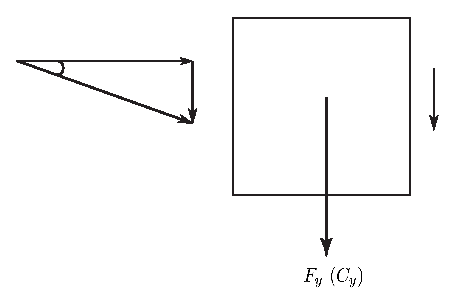
\includegraphics[width=0.5\unitlength]{../FnP/gnuplot/setup-1.eps}}         
      
      
   
 	\put(0.315,0.93){$U$}
 	\put(0.3,0.84){$U_i$}
    \put(0.42,0.88){$\dot{y}$}
    \put(0.28,0.895){ $\theta$}
    \put(0.7,0.87){\small $(+)$}
      	

 	
 	 

     

  \end{picture}

 \caption{Induced angle of attack on the square prism due to the resultant of free-stream velocity of the fluid and transverse velocity of the body.}
    \label{fig:setup_1}
\end{figure}

%\begin{figure}[!h]
\setlength{\unitlength}{\textwidth}

  \begin{picture}(1,0.4)(0,0.74)
    
  \put(0.2,0.76){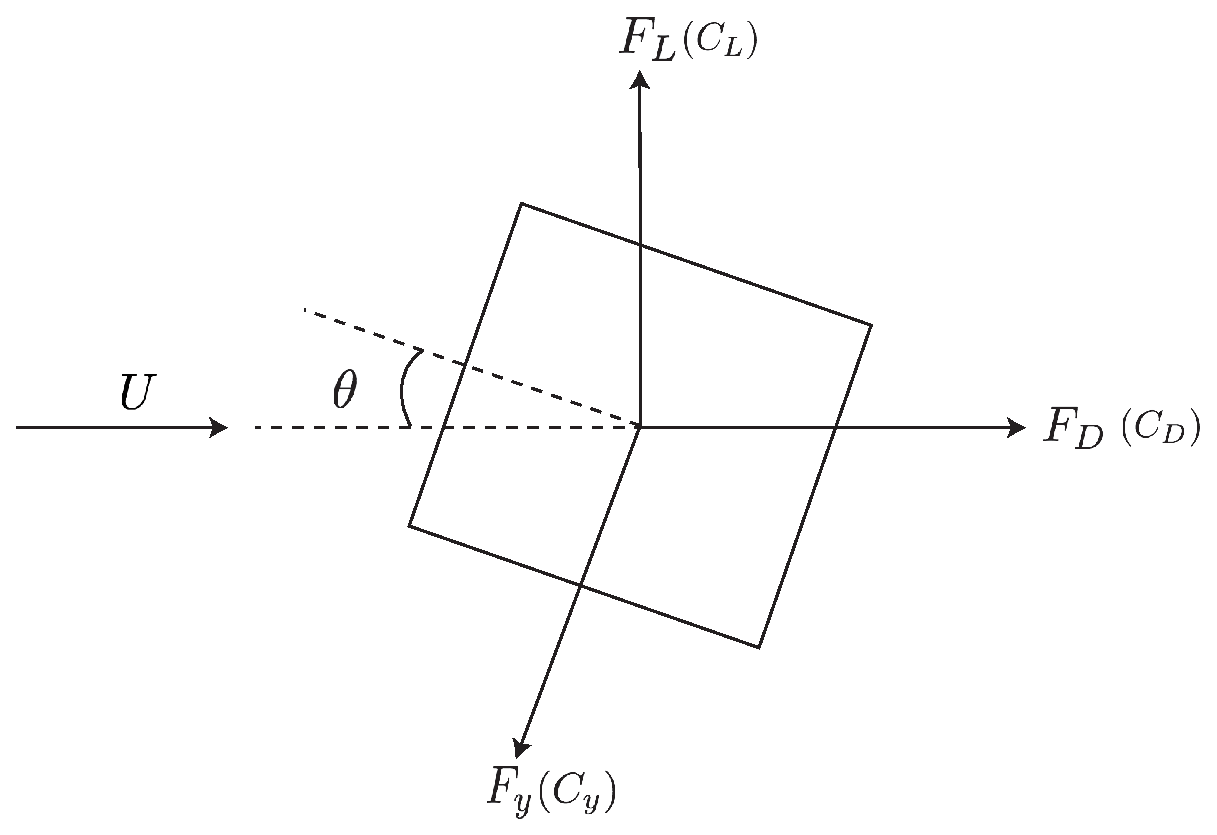
\includegraphics[width=0.5\unitlength]{./chapter-literature-revirw/fnp/f_y-illustration.eps}}         
      
      
   
% 	\put(0.315,0.93){$U$}
% 	\put(0.3,0.84){$U_i$}
%    \put(0.42,0.88){$\dot{y}$}
%    \put(0.28,0.895){ $\theta$}
%    \put(0.7,0.87){\small $(+)$}
      	

 	
 	 

     

  \end{picture}

 \caption{}
    \label{fig:f-y-sketch}
\end{figure}

A square cross section can be used as an example to further explain the galloping phenomenon. Figure \ref{fig:induced_lift_sketch}  illustrates the motion of the body at a given instant. The induced angle of attack is formed on the square cross section as a result of the free stream velocity vector $U$ and the transverse velocity vector of the body $\dot{y}$. An angle of attack implies that there will be a non-zero lift force on the body. Thus, a force is formed in phase with the velocity of the body. While illustated for the square, this mechanism can also be observed on any body that can have an angle of attack. The sign convention in this figure (and generally used in this scope of research) states that downward direction is positive.  

\subsection{Quasi-steady state theory}
\label{sec:QSS theory}


The vibrations caused in iced electric transmission lines was the key phenomenon which compelled researchers into studying fluid-elastic galloping. Some of the earlier work by \cite{Glauert1919} and \cite{DenHartog1956} lead to the pioneering study on galloping by \cite{Parkinson1964} which produced a mathematical model for a system under the influence of fluid-elastic galloping. A non-linear oscillator model was developed by Parkinson and Smith to predict the response of the system. Since then, this model has been widely used in almost all subsequent studies on galloping. Essentially, the model assumes the flow is quasi-steady. This means that the instantaneous induced lift force of the oscillating body is equal to that of the lift force generated by the same body when static at the same induced angle of attack. For the quasi-steady assumption to be valid, the conditions below have to be satisfied.

\begin{itemize}
 \item The velocity of the body does not change rapidly
 \item There is no interaction between vortex shedding and galloping
\end{itemize}

Both of these conditions imply that the vortex shedding frequency must be much higher than the galloping frequency.

The oscillator equation was solved using the Krylov and Bogoliubov method \citep{Parkinson1964}. The results obtained from experiments, carried out at $\reynoldsnumber=2200$ and a mass ratio (\mstar) around 1164 had a good agreement with the theoretical data which is shown in figure \ref{fig:parkinson_paper_data}. The details of this quasi-steady model are provided in section \ref{sec:qss_model}.

\begin{figure}
	
  \setlength{\unitlength}{\textwidth}

        \begin{picture}(1,0.82)(0,0.4)

      % % % Parkinson Data 

      \put(0.05,0.39){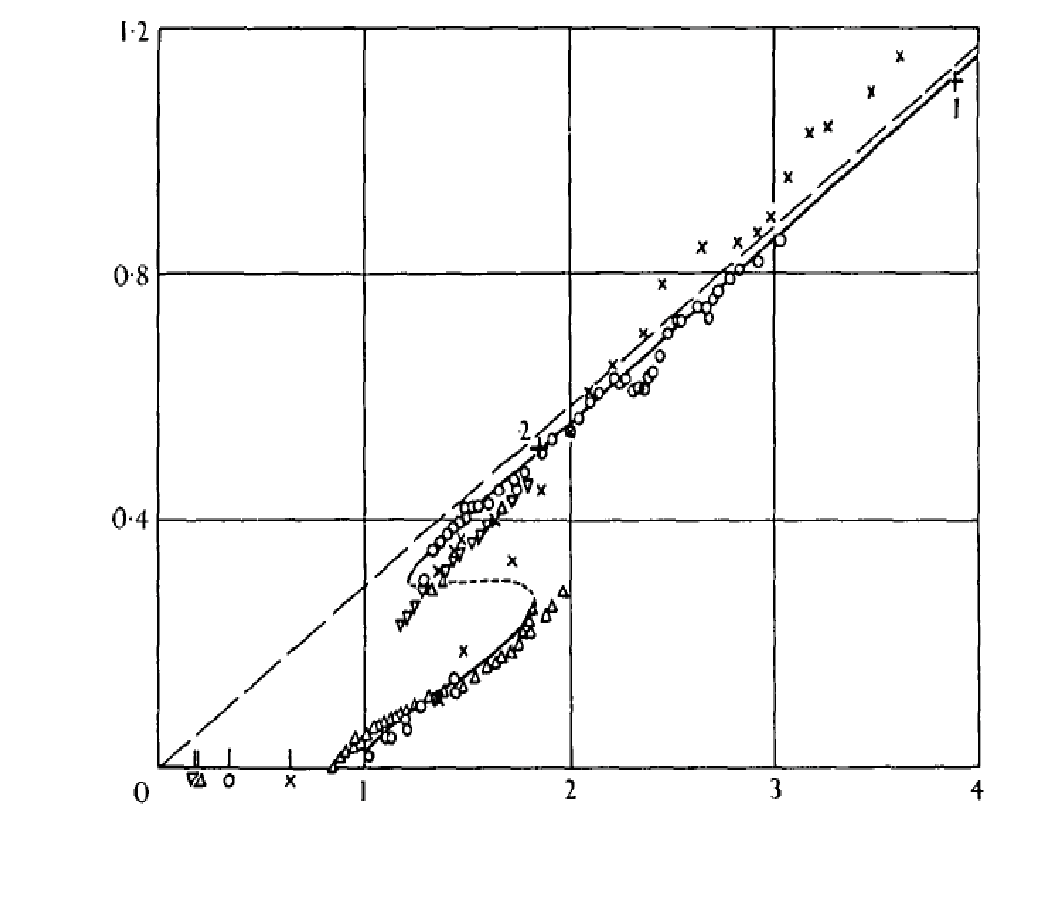
\includegraphics[width=0.9\unitlength]{./chapter-literature-revirw/fnp/parkinson_data.eps}}
      
%       \put(0.07,0.95){$\displaystyle\frac{V}{D}$}
%       \put(0.07,1.3){$\displaystyle\frac{A}{D}$}
       \put(0.05,0.8){\Large$\frac{nA}{2\beta}\bar{Y}_s$}
       \put(0.52,0.42){\Large$\frac{nA}{2\beta}U$}
       \
%\put(0.189,1.415){\small(a)}
%\put(0.189,1.07){\small(b)}
%\put(0.189,0.73){\small(c)}

%  


    \end{picture}

  \caption{``Collapsed amplitude-velocity characteristic. Theory: \solidrule \ stable limit cycle, \dashedrule unstable limit cycle. Experiment $\times \ \beta = .00107$, $\circ \ \beta =.00196$,\ $\vartriangle \beta=.00364$,$\triangledown \ \beta = .00372$,\ $+1 \ \beta=.0012$,\ $+2 \ \beta=.0032$ Reynolds numbers $4,000-20,000$ ". Figure extracted from \cite{Parkinson1964}. $\frac{nA}{2\beta}\bar{Y}_s$ is the dimensionless displacement amplitude parameter and $\frac{nA}{2\beta}U$ is the reduced velocity.$\beta$ is the damping ratio and $n=\frac{1}{\mstar}$. The experimental data shows a good agreement with the theoretical model.}
    \label{fig:parkinson_paper_data}
\end{figure}

 %vspace{10cm}


Figure \ref{fig:parkinson_paper_data} shows the comparison of data between the mathematical model and the experimental data of \citep{Parkinson1964}. The data shows a good agreement between the model and the experiments.  

\subsubsection*{Quasi-steady state oscillator model}
\label{sec:qss_model}

A simple transversely oscillating system with external driving force could be modelled with a spring, mass, damper system which can be expressed as,   

\begin{equation}
\label{equationofmotion_1}
m\ddot{y}+c\dot{y}+ky=\mathcal{Q},
\end{equation}

where the forcing term $\mathcal{Q}$ is the external force which drives the system.

Thus, the quasi-steady equation of motion of a transversely oscillating body under galloping, with linear springs and damping could be expressed by replacing the forcing term with the induced force (explained in section \ref{sec:QSS theory}) and could be expressed as,  

\begin{equation}
\label{equationofmotion}
m\ddot{y}+c\dot{y}+ky=F_y,
\end{equation}
where the forcing term $F_y$ is given by
\begin{equation}
\label{lift equation}
F_y=\frac{1}{2}\rho U^2\mathcal{A}C_y.
\end{equation}

As explained in section \ref{sec:QSS theory}, the quasi-steady assumption uses the stationary $C_y$ data for varying angles of attack as inputs to the oscillator equation. \citet{Parkinson1964} used a $7^{th}$ order odd curve fit to interpolate the stationary $C_y$ data as a function of the angle of attack. The order of the polynomial can be chosen arbitrarily depending on the study. For example \citet{Barrero-Gil2009,Barrero-Gil2010a} used a $3^{rd}$ order polynomial in order to simplify the analytical model. However, \citet{Ng2005} pointed out that a $7^{th}$ order polynomial is sufficient as higher order polynomials do not provide a significantly better result. Using a $7^{th}$ order polynomial sees the lift coefficient as a function of the angle of attack $\theta$ modelled as

\begin{equation}
\label{cy ploynomial}
C_y(\theta)=a_1\left(\frac{\dot{y}}{U}\right)-a_3\left(\frac{\dot{y}}{U}\right)^3+a_5\left(\frac{\dot{y}}{U}\right)^5-a_7\left(\frac{\dot{y}}{U}\right)^7.
\end{equation}

By substituting this forcing function into the oscillator equation (Eq:\ref{equationofmotion}) the quasi-steady state (QSS) model can be obtained as

\begin{equation}
\label{final_equation_motion}
m\ddot{y}{+}c\dot{y}{+}ky{=}\frac{1}{2}\rho U^2 \mathcal {A} \Bigg(a_1\left(\frac{\dot{y}}{U}\right){-}a_3\left(\frac{\dot{y}}{U}\right)^3{+}a_5\left(\frac{\dot{y}}{U}\right)^5{-}a_7\left(\frac{\dot{y}}{U}\right)^7 \Bigg).
\end{equation}

As the current study is focused on the low \reynoldsnumber\ region, it is a known fact that the vortex shedding will be well-correlated along the span and therefore provide a significant forcing. \citet{Joly2012} introduced an additional sinusoidal forcing function to the model in order to integrate the forcing by vortex shedding. By the addition of this forcing \citet{Joly2012} managed to obtain accurate predictions of the displacement amplitude even at low mass ratios, where the galloping is significantly suppressed by the vortex shedding to the point that it is no longer detectable. However, the strength or the amplitude of this sinusoidal forcing needed to be tuned in an \emph{ad hoc} manner, and the relationship between this forcing and the other system parameters was not clear. Thus in the current study this forcing is not used.


\subsubsection*{Presence of hysteresis}


\cite{Parkinson1964} observed a hysteresis region when the displacement amplitude was plotted as a function of the reduced velocity. Essentially two amplitudes were observed for the same reduced velocity depending on the initial condition. This fact is quite vital for energy harvesting as two values of energy levels can present for the same reduced velocity. Thus, have to be careful in considering the initial conditions of the system to gain a higher power output.  

Although hysteresis was observed in the amplitude data of \cite{Parkinson1964}, the studies carried out by \citet{Barrero-Gil2009} and \citet{Joly2012} at much lower Reynolds numbers ($159\leq \reynoldsnumber\leq 200$), did not show any hysteresis. \citet{Luo2003} concluded that hysteresis was present due to the presence of an inflection point in the $C_y$ curve which was only observed at high Reynolds numbers (\citet{Parkinson1964} data) and was not present at lower Reynolds numbers. It was further explained by \citet{Luo2003} the cause of this inflection point which was the intermittent reattachment of the shear layer at certain angles at occurred at high Reynolds numbers.   
 
\begin{figure}
	
  \setlength{\unitlength}{\textwidth}

  \begin{picture}(1,0.9)(0,0.75)

      % % % Parkinson Data 

      \put(-0.15,0.2){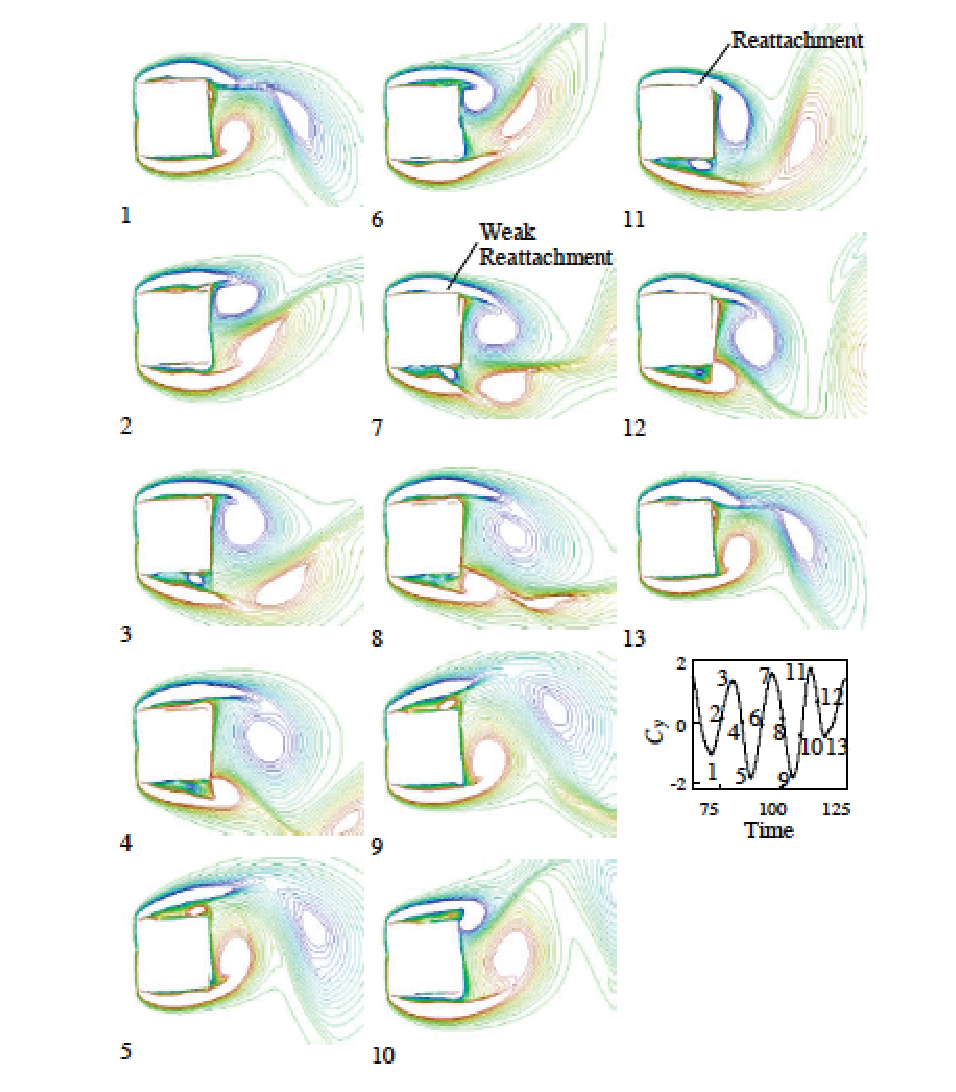
\includegraphics[width=1.3\unitlength]{./chapter-literature-revirw/fnp/luo-re-attachment.eps}}
      
%       \put(0.07,0.95){$\displaystyle\frac{V}{D}$}
%       \put(0.07,1.3){$\displaystyle\frac{A}{D}$}
      
%\put(0.189,1.415){\small(a)}
%\put(0.189,1.07){\small(b)}
%\put(0.189,0.73){\small(c)}

%  


    \end{picture}

  \caption{\label{fig:lit-review-luo-reattachment-1}Vorticity contours of \cy\ and the corresponding time for $\reynoldsnumber=1000$, $\theta=2^{\circ}$ extracted from \citet{Luo2003}. The intermittent shear level is visible in points 7 and 11}
\end{figure}


 %vspace{10cm}


Figure \ref{fig:lit-review-luo-reattachment} shows the vorticity contours of a square cross section obtained at various points of the vortex shedding cycle, at $\reynoldsnumber=1000$, $\theta=2^{\circ}$ obtained from \citet{Luo2003}using the  diffusion-vortex method and vortex-in-cell method. The points 7 and 11 show the intermittent shear layer reattachment which causes the hysteresis in the \cy\ vs. $\theta$ curve at high Reynolds numbers.

\vspace{20mm}   

\subsection{Induced force and the shear layers}
\label{subsec:c_y and shear layers}

 The quasi-steady model has already been validated and re-validated by many studies \citep{Parkinson1964,Barrero-Gil2009,Luo2003} and proven to model galloping. Since this model essentially assumes that the system is quasi-steady, the mean flow-field data of static body simulations at various angles of incidence can be used to analyse the behaviour of the instantaneous flow field of a galloping system at the same instantaneous induced angle. 
 
 
\begin{figure}[h]
\setlength{\unitlength}{\textwidth}

  \begin{picture}(1,0.46)(0,0.75)
    
  \put(0.2,0.76){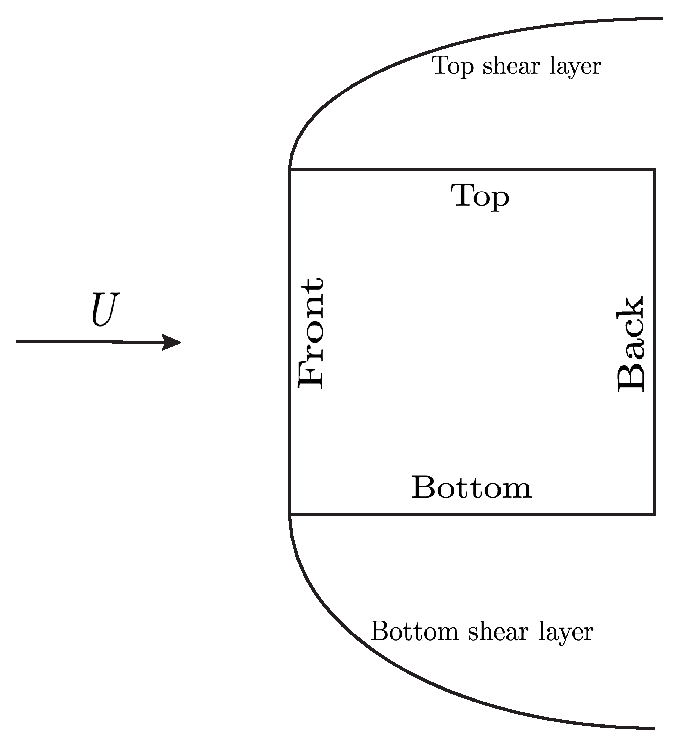
\includegraphics[width=0.4\unitlength]{./chapter-literature-revirw/fnp/shear-layer-sketch.eps}}         
      
      
   
 
 	
 	 

     

  \end{picture}

 \caption{Illustration of the top and bottom shear layers.}
    \label{fig:shear-layer-sketch}
\end{figure}

\begin{figure}[t!]

  \setlength{\unitlength}{\textwidth}

  \begin{picture}(1,0.35)(0,0.725)

    \put(-0.01,0.76){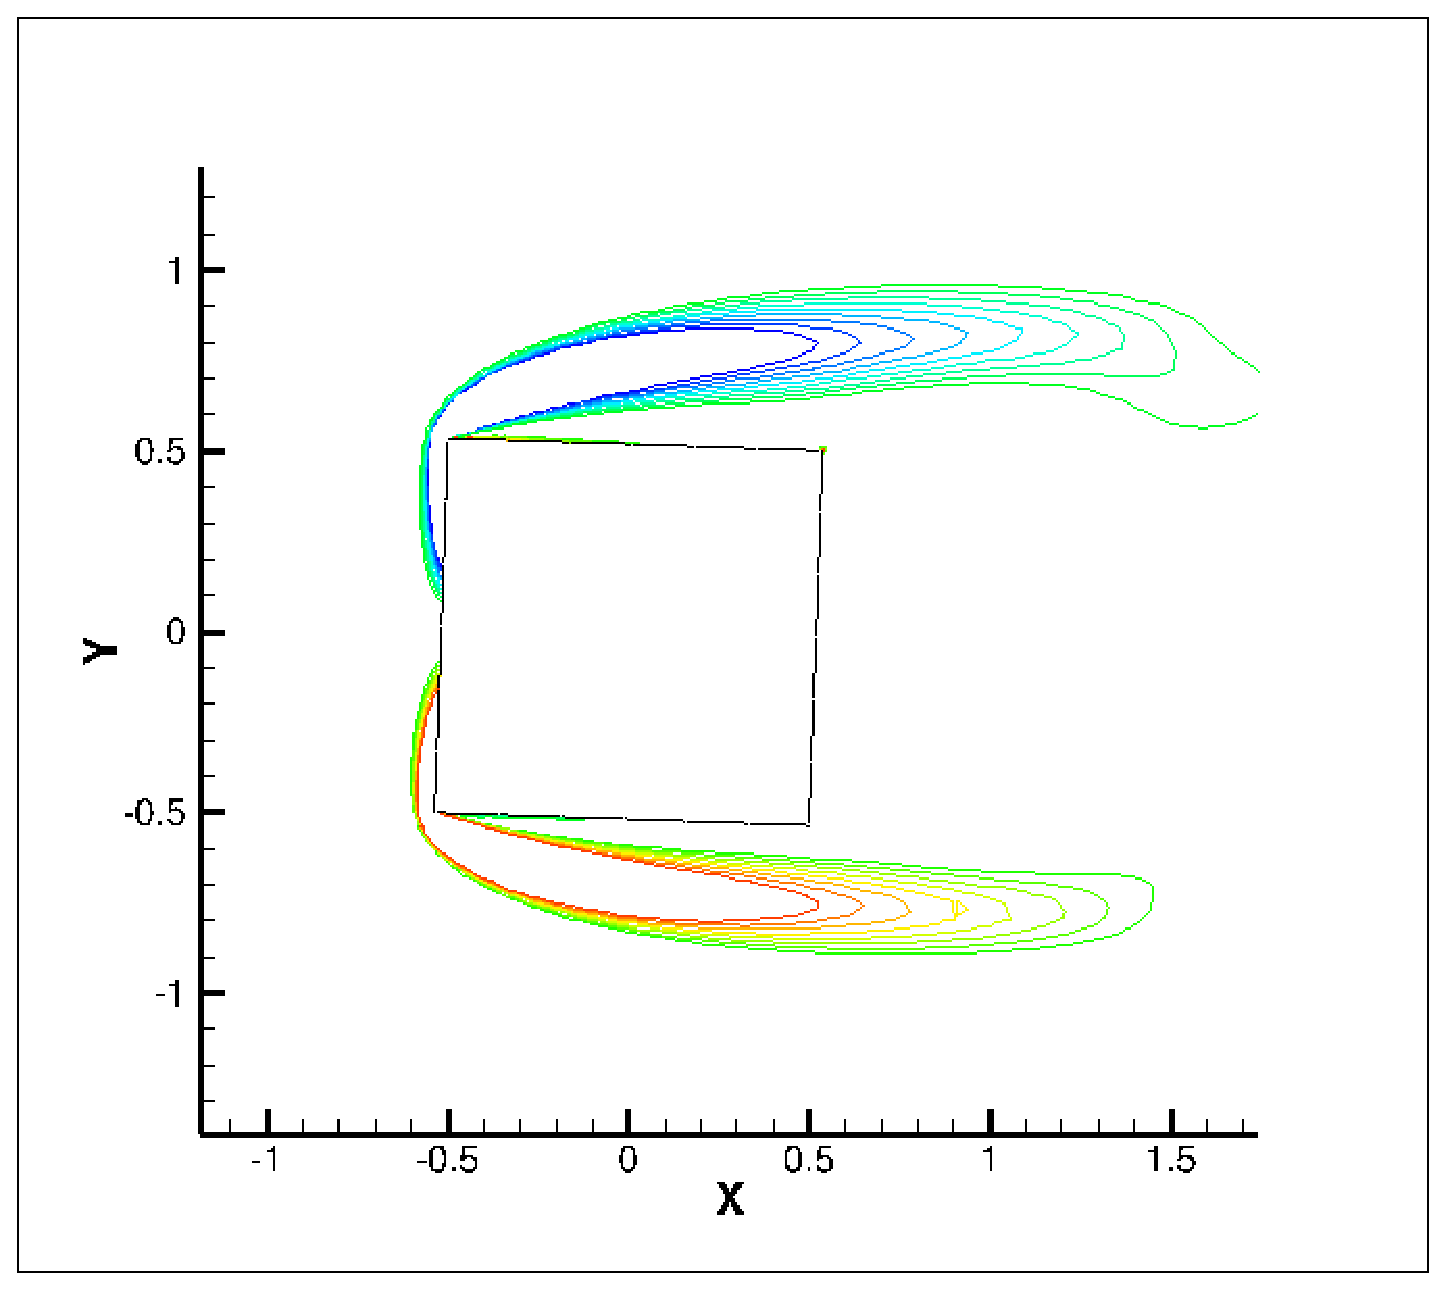
\includegraphics[width=0.33\unitlength]{./chapter-literature-revirw/fnp/square-2.eps}}
    \put(0.335,0.76){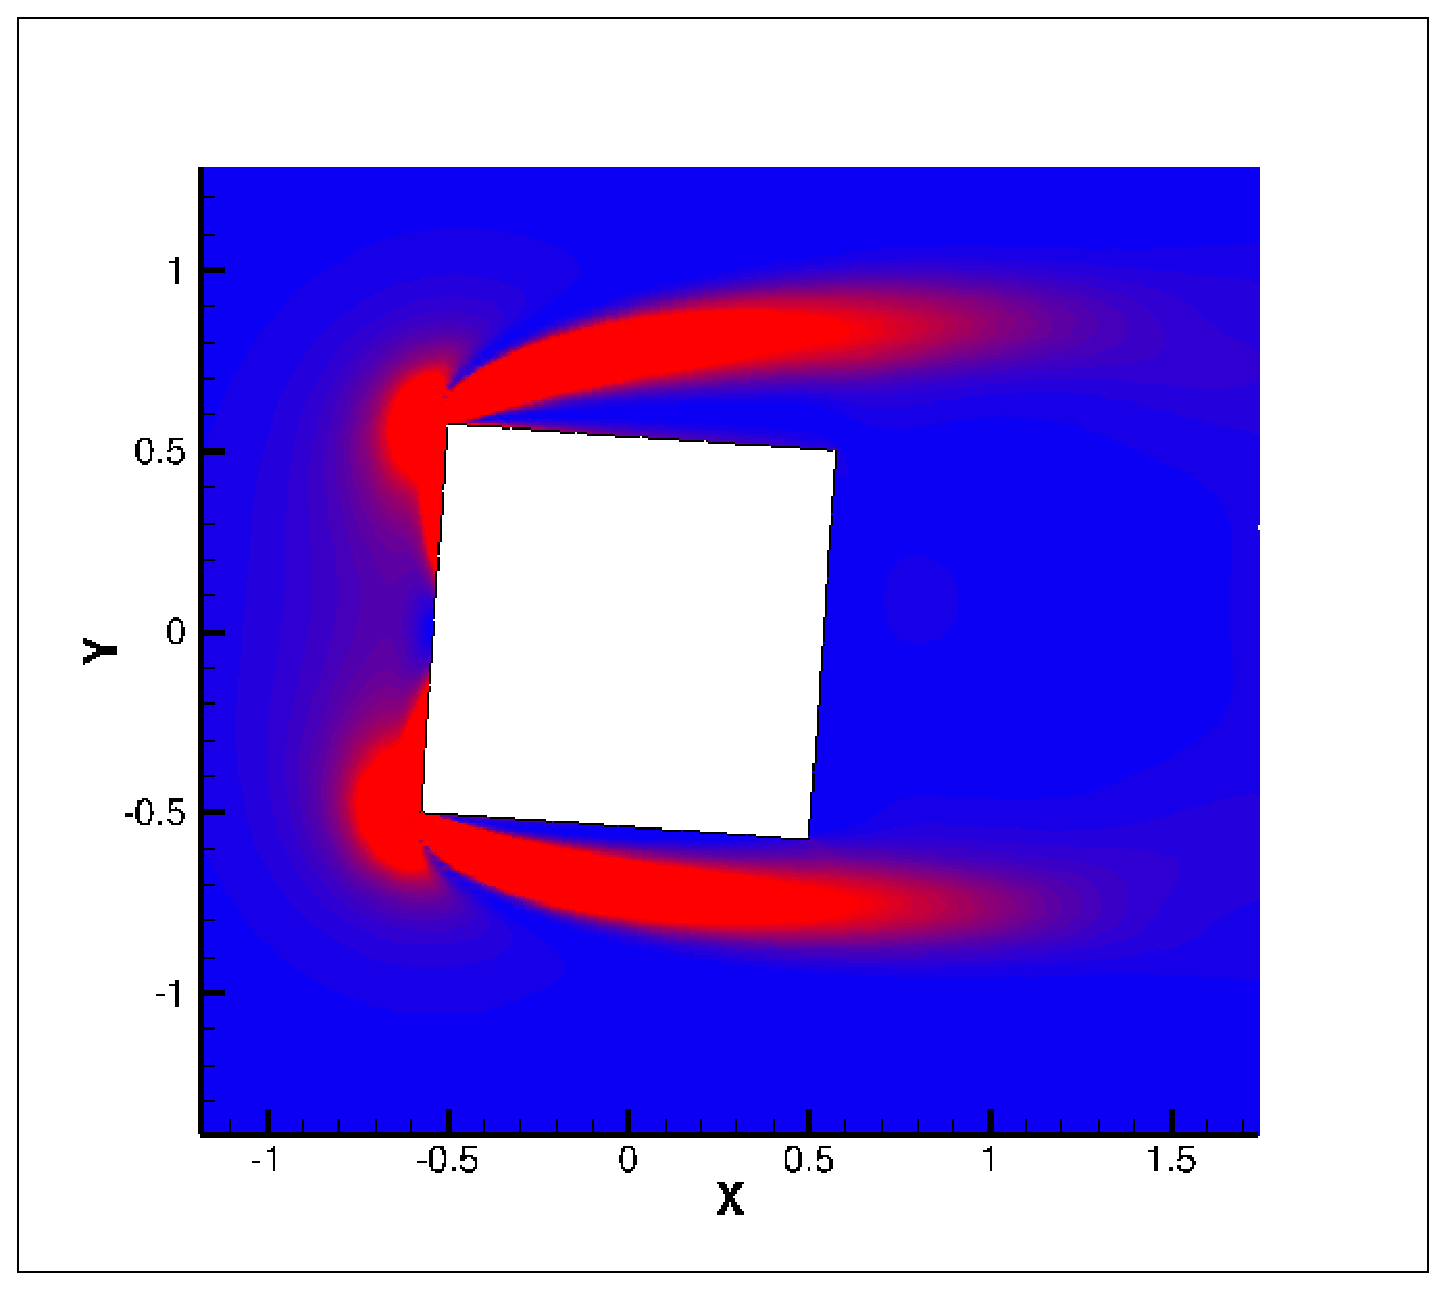
\includegraphics[width=0.33\unitlength]{./chapter-literature-revirw/fnp/square-4.eps}}
    \put(0.68,0.76){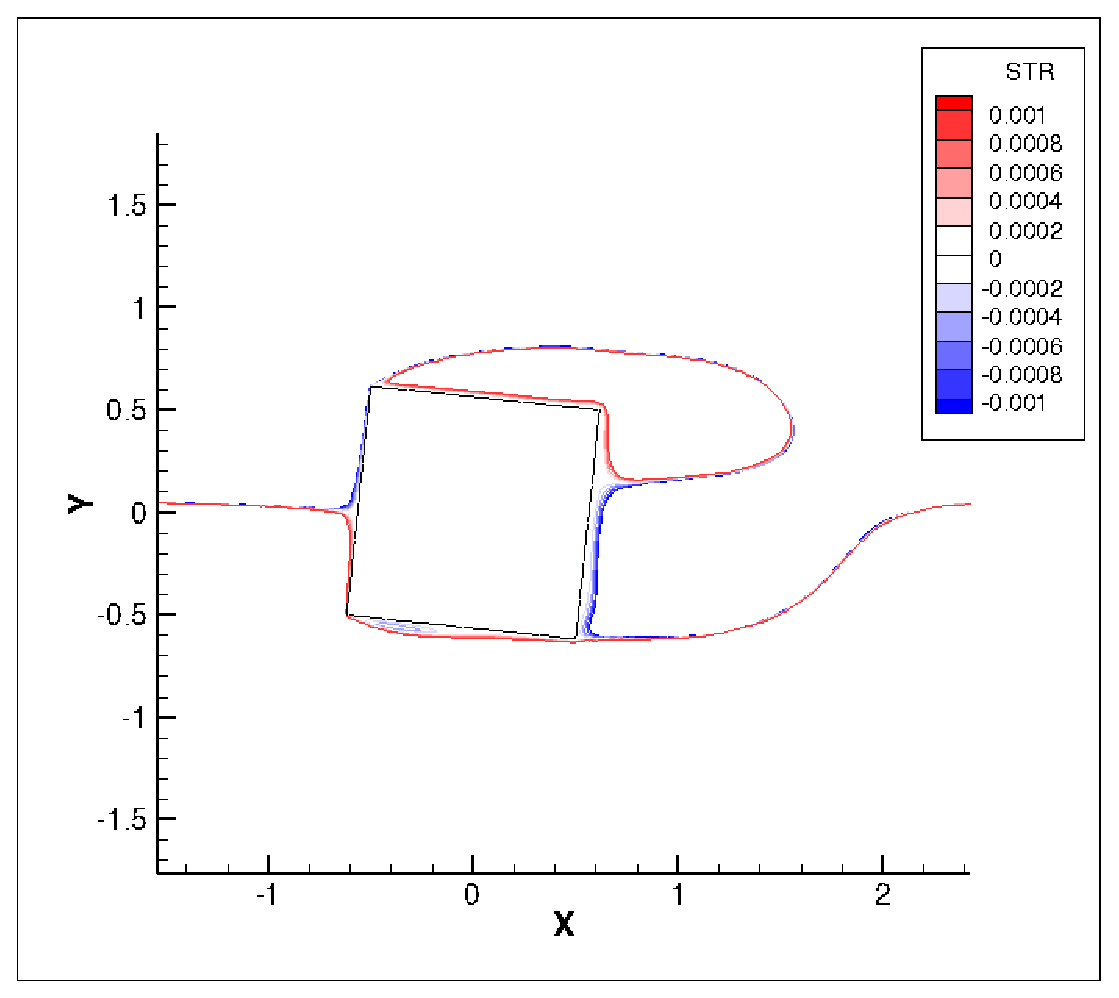
\includegraphics[width=0.33\unitlength]{.//chapter-literature-revirw/fnp/square-6.eps}}

   
    
    \put(0.0,0.735){(a)}    
    \put(0.34,0.735){(b)}
    \put(0.685,0.735){(c)}
  
  \end{picture}

  \caption{Stream functions of time averaged flow field on a stationary square section at $\reynoldsnumber=200$ at different incidence angles. (a) $2^{\circ}$ ($C_{y}$ increases),(b) $4^{\circ}$ ($C_{y}$ peaks) and (c) $2^{\circ}$ ($C_{y}$ decreases). The bottom shear layer comes closer to the bottom wall and reattaches as the angle of incidence increases.}
  \label{fig:shear_layers}
\end{figure}







\citet{Paidoussis2010,Parkinson1964,Barrero-Gil2010a} and many other published studies state that a system which sustains galloping should satisfy the condition that $\partial C_y/\partial \theta>0$, i.e, an upward motion from the equilibrium position should induce an upward lift force. The mean induced lift (\cy) occurs due to the unbalanced pressure distribution on the top and bottom sides of the afterbody of the cross section (refer figure \ref{fig:shear-layer-sketch}) when a small transverse velocity is given \citep{Parkinson1989}. This pressure difference of the afterbody is a result of the relative proximity of the top and bottom shear layers (illustrated in figure \ref{fig:shear-layer-sketch}) to the respective sides of the body. 

Contour plots of the shear strain rate magnitude, which is directly proportional to shear stress, for a static square cross section at various incidence angles shown in figure \ref{fig:shear_layers} clearly shows the behaviour of the shear layers at either sides of the body. Data are presented for three key incidence angles $2^{\circ}, 4^{\circ} \text{and}\ 6^{\circ}$. In comparison with figure \ref{fig:lift_curves} these points can be identified as being in regions where \cy\ initially increases, \cy\ is maximum and \cy\ decreases. 

As the angle of incidence ($\theta$) increases clockwise from $2^{\circ}-6^{\circ}$, it can be clearly observed in figure \ref{fig:shear_layers} that the bottom shear layer comes closer to the bottom wall of the body compared to the top shear layer. The shear layer nearer to the body creates higher suction compared to the shear layer at the opposite side, as the higher velocity in the shear layer implies a lower pressure, from a simple Bernoulli-type argument. This pressure imbalance between the top and bottom sides of the body creates a downward force which with the sign convention introduced in figure \ref{fig:induced_lift_sketch} is positive. As the angle is further increased to $\theta=4^{\circ}$, the bottom shear layer comes even closer and therefore the pressure difference becomes greater leading to a higher $C_{y}$. The induced lift force \cy, becomes maximum when the shear layer near to the wall just reattaches at the trailing edge. As $\theta$ is further increased at  $\theta=4^{\circ}$ (figure \ref{fig:shear_layers} (b)), the recirculation region formed by the reattachment of the bottom shear layer shrinks in size resulting in a reduction of the velocity near the wall, and therefore an increase in pressure. This implies a reduction of the pressure imbalance between the top and bottom surface leading to the reduction in $C_{y}$. This theory has been discussed in \citet{Parkinson1989}. The variation of \cy\ vs $\theta$ is presented in figure \ref{fig:lift_curves}. As the body is connected to an oscillatory system (discussed in section \ref{sec:exci-galloping}), this shear layer behaviour also harmonizes with the cyclic behaviour of the system providing the driving force to the system so that the motion of galloping is sustained.

\subsection{Governing parameters of galloping \KJ{I need a better heading than this....}}

From the published literature, it is observed from the earlier works such as \citet{Parkinson1961,Luo1994} to recent studies such as \citet{Luo2003,Barrero-Gil2010a,Joly2012} that classical VIV parameters have been incorporated to describe galloping. These parameters are the reduced velocity \ustar\ which is the velocity of the flow normalised by the natural frequency of the system and $\zeta$ which is the damping ratio based on the linear system in a vacuum. Both of these parameters consists of a frequency component. As VIV is a resonant type of phenomenon these parameters are suitable for VIV. However, as galloping is not a resonance-type phenomenon driven by the natural frequency, but a velocity driven phenomenon, these normalisations might not be suitable for galloping. This could be clearly observed in \citet{Barrero-Gil2010a}. In this study, which is focused on energy harvesting, the power curves presented using these current parameters does not provide a good collapse. Therefore, it is necessary to formulate new parameters which effectively describe galloping particularly the energy transfer between the fluid and the body as it is the focus of this study.     


\subsection{Frequency response}
 
 It is clear that the cyclic motion of the shear layer will harmonize with the mechanical system. Therefore, the frequency response should be close to the natural frequency of the system $\omega_{n}$ \citep{Paidoussis2010}. This is significantly different from the VIV mechanism, where the primary frequency comes from the periodic forcing of the vortex shedding. Hence, in the QSS model the natural frequency of the system can be identified as the frequency of oscillation. However, it should be  noted that this is valid on the regimes where the conditions discussed in section \ref{sec:QSS theory} are satisfied. 
 
 The experimental studies carried by \citet{bouclin:77} concluded at high reduced velocities with large inertia (where the natural frequency is very low), the motion of the body controls the frequency of the system rather than the vortex shedding. The structural damping has no effect provided that it is small. This study also concluded that as the inertia and the reduced velocity gets lower, there is some interaction between vortex shedding and galloping. When this occurs the frequency is mainly governed by the vortex shedding. 
 
 \subsection{Fluid mechanics governing the galloping response}
 \label{subsec:fluid_mechanics_of_galloping}
 
 As discussed in subsection \ref{subsec:c_y and shear layers} the driving force of a galloping system is the asymmetrical placement of the shear layers at either sides of the body. As a consequence, it is clear that a significant afterbody is needed for the shear layer interaction to sustain galloping. \citet{Parkinson1974,Parkinson1989} and \citet{Bearman1987} have discussed well the importance of the length and the shape of the body for galloping in their reviews. It is also highlighted in \citet{Parkinson1974} that the most important physical parameters for galloping are the size relative to the characteristic height and the shape of the afterbody. Manipulating the shape of the afterbody and thereby manipulating the shear layer interactions with the body, gives the ability to control the galloping response.
 
\citet{Blevins1990} provided a good comparison of the shapes which are prone to galloping based on the work by \citet{Parkinson1961}, \citet{Nakamura1975a} and \citet{Nakamura1977}. The reproduction of Blevins's data can be found in \citet{Paidoussis2010} and presented in figure \ref{fig:par_diff_cross_sec}. Here the induced angle is represented by $\alpha$ and the transverse force force coefficient is represented by $C_{fy}$. In order for galloping to sustain, the direction of both of these quantities should be same this thus have to satisfy the condition of 

\begin{equation}
\frac{\partial C_{fy}}{\partial \alpha } >0
\end{equation}  
    
 \begin{figure}
	
  \setlength{\unitlength}{\textwidth}

\fbox{
        \begin{picture}(1,1.2)(0,0.5)

      % % % Parkinson Data 

      \put(0.05,0.52){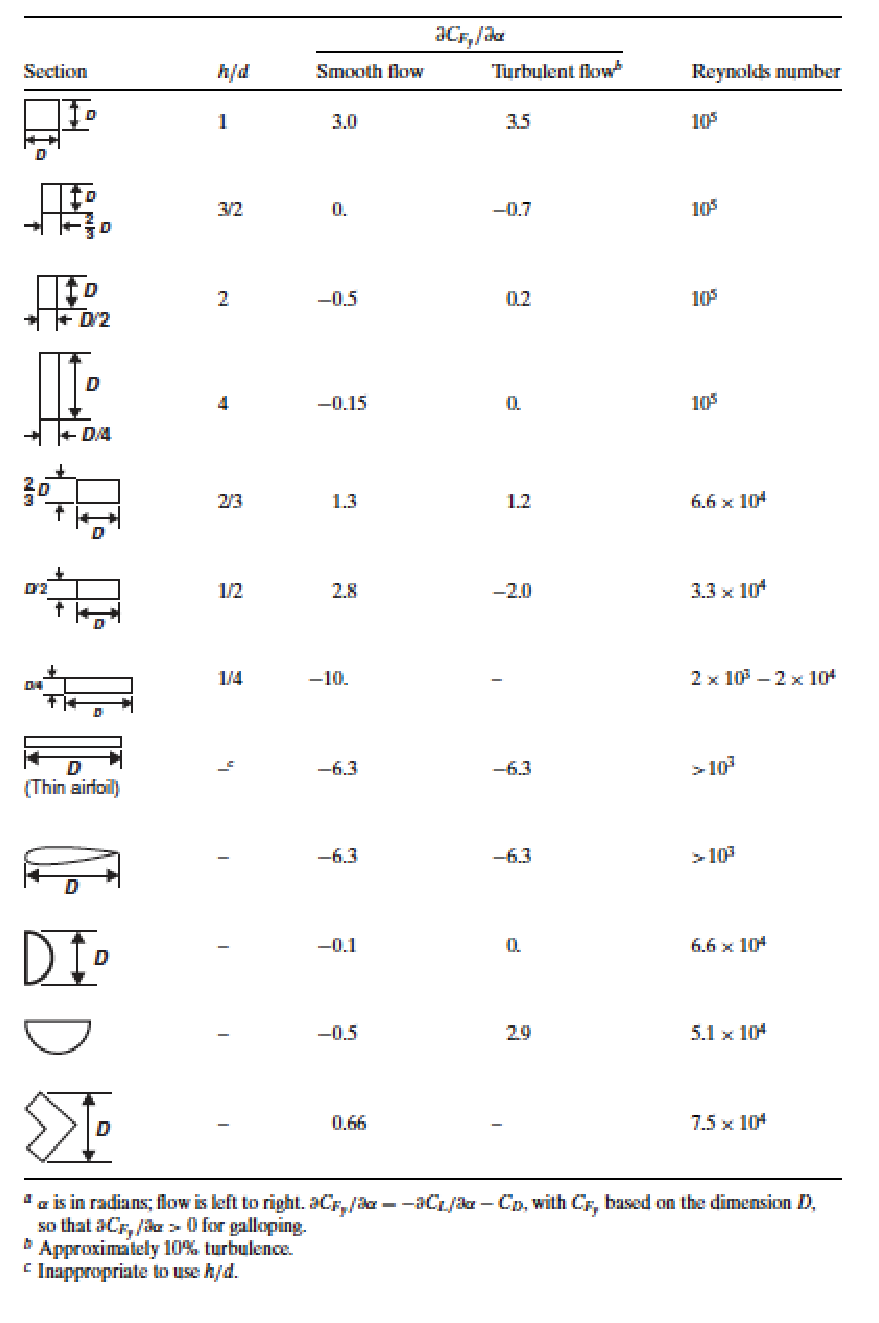
\includegraphics[width=0.75\unitlength]{./chapter-literature-revirw/fnp/per_cross_sec.eps}}
        


    \end{picture}
}
  \caption{ ``The transverse force coefficient for various sections in steady smooth or turbulent flow (after \citet{Blevins1990})" obtained from \citet{Paidoussis2010}. Here the induced angle is represented by $\alpha$ and the transverse force force coefficient is represented by $C_{fy}$. In order for galloping to sustain, the direction of both of these quantities should be same and thus have to satisfy the condition of $\frac{\partial C_{fy}}{\partial \alpha } >0$.}
    \label{fig:par_diff_cross_sec}
\end{figure}

 %vspace{10cm}

 
 
\citet{Naudascher1993}, \citet{Ruscheweyh1996}, \citet{Deniz1997} and \citet{Weaver2005} also provide data on different cross sectional shapes. \citet{Alonso2009} carried out wind tunnel tests on biconvex and rhomboidal cross sections. This study concluded that the galloping stability is dependent on the angle of attack. The aspect ratios where galloping is sustained in these cross sections were identified. Studies were further carried out by Alonso for elliptical cross sections \citep{Alonso2010} which concluded that galloping is Reynolds number dependent for elliptical cross sections. The study of triangular cross sections carried out by \citep{Alonso2005} isolated the angles of attack where galloping is sustained. The regions of stability for galloping at different angles of attack and the static force coefficients are presented in these studies with regards to the cross section involved. \citet{Luo1994} carried out an interesting study where the influence of the afterbody on galloping was investigated. The sides of a square section was chamfered gradually delaying the shear layer re-attachment, and two trapezoidal cross sections and one isosceles triangle was obtained. The \cy\ vs. $\theta$ plots revealed that the maximum value of \cy\ increased as the chamfering angle increased (i.e when the cross section was transformed from a square to a isosceles triangle). Anther interesting observation was that the incident angle where maximum \cy\ occurred increased as the chamfering angle increased. Delaying shear layer reattachment leads to higher \cy\ at higher induced angles which leads to higher induced velocities. This fact is beneficial for energy harvesting because as shown in equation \ref{eqn:power_alt} power is a function of both $F_{y}$ and the velocity of the body. \citep{Kluger2013} concluded that the best cross sectional shape for their "vibro-wind'' energy harvester was a trapezoidal cross section. However, this study has not revealed the underpinning fluid mechanics in detail such as the behaviour of the shear layers which makes an optimum cross section.

While many of these previous studies have investigated the influence of different body shapes on the galloping response, very few have systematically varied the shape of the body with the aim of deliberately amplifying the galloping. If galloping is to be used as an energy harvesting mechanism, finding an optimum body shape which produce large transverse velocities is desirable.


\subsection{Galloping as a mechanism of energy harvesting}

The focus of fluid-elastic galloping research in the past was on understanding and developing methods to suppress it, due to the adverse effects on civil structures. However, recently the focus of research has been redirected to develop mechanisms to excite galloping rather than suppressing it. This is due to the recent demand for alternative energy sources with minimal environmental impact. Thus, this demand for alternate energy has lead researchers to develop ways of extracting useful energy from flow induced vibrations.

Bernitsas and his group in the University of Michigan have made significant progress on using VIV as potential candidate for energy extraction. \cite{Bernitsas2008a-concept} introduced the concept of using VIV as a mode of energy extraction. The group have developed a device called VIVACE converter based on this concept. The work has been further expanded to focus on various aspects (such as Reynolds number effects, damping effects etc.) in \citet{Bernitsas2009,Raghavan2009,Raghavan2010a,Lee2011a}. This group has studied extensively on the effect of the mechanical parameters, the Reynolds number effects and the bottom boundary conditions of the VIVACE converter, in order to obtain efficient energy output using VIV as an energy harvesting mechanism. 

In contrast, the research carried out investigating the possibility of energy harvesting using fluid-elastic galloping is quite limited. \citet{Barrero-Gil2010a} conducted the pioneering study on energy harvesting using fluid-elastic galloping. The key consideration investigated in this study was that unlike VIV fluid-elastic galloping is not dependent on a synchronisation or a ``lock-in" mechanism. Therefore, it could operate on a wide spectrum of frequencies giving fluid-elastic galloping an advantage over VIV as a mechanism of energy harvesting. The study incorporated the QSS model where the Krylov and Bogoliubov method was used to solve the equation. This study used a $3^{rd}$ order polynomial rather than a $7^{th}$ order polynomial for simplification purposes which would have lead to less accurate quantitative results. However, This initial work showed that galloping could indeed used as a candidate for energy harvesting .\citet{vicente-Ludlam2014} showed that there is a link between the optimal electrical load resistance and the flow speed. This study was built on \citet{Barrero-Gil2010a} taking the QSS model as the mode of data acquisition. Similar to \citet{Barrero-Gil2010a} this study also incorporated a low order $3^{rd}$ order polynomial for the QSS model which again restricted the quantitative accuracy of the results. Since the work was mainly qualitative, it was identified that the understanding is primary and therefore step-by-step research has to be conducted in order to properly understand the link between energy transfer in the galloping mechanism and a experimental prototype should be developed to test the engineering performance. 

\citet{Kluger2013} from Cornell university have produced a prototype called "Vibro-wind" energy harvester which essentially uses the galloping mechanism. The mechanism used here differ slightly from the traditional transversely body where the oscillating body is connected with a cantilevered beam. Thus, there is both translational and rotational motion in the system. It was concluded that the amplitude of the galloping oscillator which couples the rational motion with the translational motion was always less that the amplitude of a body under a pure translational motion. As the present study is focused on theoretical aspects of the energy transfer, motion of the body is kept purely translational.   


\subsection{Review summary and statement of objectives}

 It is clear that more investigations should be carried out on energy transfer of a galloping system, particularly to develop efficient energy harvesting systems. More fundamental research is needed to explore the underpinning effects of mechanical and fluid dynamic parameters influencing the energy transfer of a galloping system to fill the gaps of the existing knowledge base. Thus, the objectives of the current research, spread over two phases, are defined as follows.
 
 \subsection*{Phase 1: Understand the governing mechanical parameters of the system and isolate regions of parameter space where a good power transfer can be obtained}
 
 \citet{Paidoussis2010} describes galloping as a ``velocity dependent damping controlled phenomenon". Yet, so far the scaling parameters used in studies are the traditional VIV parameters which are the damping ratio $\zeta$ and the reduced velocity \ustar\ \citep{Barrero-Gil2010a} which has a embedded frequency component. Thus following objectives were defined for this phase 
 
 \begin{itemize}
\item Formulate a new set of scaling parameters based on the natural time-scales of the system.
\item Investigate the influence of these parameters on mean power transfer.
\item Isolate the regions where high power transfer can be obtained.
\item Investigate the relationship between these new scaling parameters and the frequency response of the system. 
 \end{itemize}
 
    
  \subsection*{Phase 2: Understand the fluid mechanics of the system and optimise and control these mechanics to obtain a higher power transfer}
  
  \citet{Luo1994} showed that inhibition of shear layer reattachment could lead to higher peak $F_{y}$ at higher induced angles and therefore higher transverse velocities. Thus, from equation \ref{eqn:power}, it can be hypothesised that a higher mean power can be obtained by inhibition of the shear layer reattachment. Hence, the following objectives were defined for phase 2. 
  
  \begin{itemize}
  	\item Obtain QSS power data by systematically delaying the shear layer and investigate the influence on power.
  	\item Identify the relationship between the flow structures and the mean power output through analysis of the flow-field.
  	\item Provide design considerations for a galloping energy extraction system based on passive control of the shear layers. 
  \end{itemize}
 
 
 The stated aims are addressed by the following sections. Objectives of phase 1 are addressed in chapter \ref{chap:pi_1_pi2}. A new set of scaling parameters namely the combined mass stiffness \massstiff\ and the combined mass damping \massdamp\ are formulated from the linearised QSS model. The power data of obtained from numerically solving the QSS model and direct numerical simulations are presented though the new parameters and compared against the classical VIV parameters. Furthermore, an expression for the frequency of the system is formulated in terms of \massstiff\ and \massdamp. The data obtained though this model are compared against data acquired though QSS model and DNS. 
 
 
 Chapter \ref{chap:cross-sections} addresses the objectives of phase 2, where the possibility of achieving higher power transfer though the inhibition of shear layer reattachment is investigated. The inhibition of the shear layer reattachment is achieved by altering the afterbody of the square cross section. The mean power data of these cross sections obtained using the QSS model and DNS are analysed and compared. Key regions of the \cy\ vs. $\theta$ curve which significantly influences the power transfer are analysed and compared. Through this comparison, design considerations for an efficient galloping energy harvesting system are discussed.        
%ƒ\textbf{}
\chapter{Methodology and validation}

\section{Introduction}
 
An overview of the modeling and the computational methods used in this study are presented in this chapter. This study uses well established techniques to model and study fluid elastic galloping. Therefore, only a brief overview is provided together with relevant references where the development and vigorous validation has been presented.  

This chapter is presented in the following order. The equations used to model the system are presented and discussed. Next, a brief discussion of the techniques used for direct numerical simulations are presented, followed by the problem formulation and the discussion of the parameters used. Finally, validation data are presented and discussed to demonstrate the accuracy of the direct numerical simulations.


\subsection{Parameters used}

The findings in this study are presented in two categories i.e. high and low Reynolds numbers, so as to study the system at laminar and turbulent flow regimes. One of the main objectives in this study is to capture the essential flow physics which governs galloping accurately through direct numerical simulations. Detailed data could be obtained on sensitive parts of the flow-field such as the shear layer through by computational methods, in particular Direct Numerical Simulation (DNS) compared to experimental methods. However, DNS becomes computationally intractable at high Reynolds number. Thus, a major portion of the study was carried out in the laminar range where the flow is laminar and two dimensional. It is possible to carry out 3-dimensional simulations at the turbulent regions. However, this demands a large number of nodes (in the range of millions) and a longer computational time (in the range of months for a single simulation) to gain an accurate result and thus, the laminar 2-dimensional regime was selected.

A second modelling technique employed is the numerical integration of
a low-order, but nonlinear, equation of motion derived using a
quasi-static assumption \citep{Parkinson1964}. This model only requires force data obtained from static body simulations or experiments. Therefore, although a majority of the study is focused on the low Reynolds number regime, some results
are presented using inputs from published data at high Reynolds
numbers to this low order model to provide a comparison between high and low Reynolds number
cases.

One crucial factor is the selection of a suitable Reynolds number for the ``low" Reynolds number regime for the simulations to be valid. Studies by \citet{tong2008} and \citet{sheard2009} reveal that the approximate value of 3-dimensional transition of the wake for a stationary square cross section is $\reynoldsnumber=160$. \citet{Barrero-Gil2010a} concluded that a high value of $a_1$ or the initial gradient of the \cy\ vs. $\theta$ curve should be high to gain an efficient energy harvesting through galloping. \citet{Joly2012} showed that this gradient is significantly higher at $Re=200$ compared to $\reynoldsnumber=160$. Furthermore, \citet{Leontini2007a} concluded that the oscillation of the bluff body essentially stabilizes the wake, for example the the limit of three-dimensional transition of an oscillating circular cylinder can be as high as $\reynoldsnumber=280$, compared to the transition Reynolds number of $\reynoldsnumber\simeq 190$ for a stationary cylinder. As the essential flow physics such as the formation of the K\`arm\`an vortex street is common for both a circular and square bluff body, it can be assumed that the wake is also stabilised for oscillating square cross sections. Thus, $\reynoldsnumber=200$ was selected as the Reynolds number for the ``low" Reynolds number region as a compromise between keeping the flow strictly two-dimensional, and providing a high enough lift to generate vigorous galloping.

 $\reynoldsnumber=22300$ was defined as the ``high'' Reynolds number in this study, which matches the pioneering study of galloping by \citet{Parkinson1964}. Therefore, the aerodynamic data for a stationary square section at this Reynolds number was obtained from the literature as input to the QSS model. For the high \reynoldsnumber\ tests, predictions of power output were obtained using the coefficients of the $C_y$  vs. $\theta$ curve from \citet{Parkinson1964} as inputs to the QSS model. Stationary $C_y$ data at different angles of attack used as inputs to the QSS model were obtained  for the low Reynolds number regime using direct numerical simulations.

The average power was obtained by using equation \ref{eqn:power}, and the averaging was done over no less than 20 galloping periods. The mass ratio $m^*$ was kept at 1163 for $\reynoldsnumber=22300$ (Similar to \citet{Parkinson1964}). Considering previous studies \citep{Robertson2003,Joly2012} \mstar\ was kept at $m^*=20$ which was a level of inertia not so high as to suppress galloping and not so low for vortex shedding to dominate and weaken galloping as observed by \citet{Joly2012}. The reduced velocity \ustar\ was kept $\ustar\geq 40$ to keep the natural frequency of the system far from the frequency of vortex shedding to ensure that the primary mode of flow-induced vibration was galloping as opposed to vortex-induced vibration (VIV). These parameters were used throughout this study unless specified otherwise.

\section{Quasi-steady model}
\label{sec:QSS_model_methodology}

The quasi-steady state model discussed in section \ref{sec:QSS theory} was used to obtain oscillator response data. The quasi-steady state model has proven its ability to obtain accurate galloping response data (as also discussed in section \ref{sec:QSS theory}). Therefore, a large number of cases can be modelled in a small amount of computational time. The oscillator equation consists of a spring, mass and damper oscillator expression with a $7^{th}$ order interpolation polynomial in terms of the body velocity (or equivalently, the instantaneous incidence angle) as the forcing function (equation \ref{final_equation_motion}), obtained from a curve fit of aerodynamic data (i.e. \cy\ as a function of the incidence angle).

\subsubsection{Solving the quasi-steady state equation}

The quasi-steady model being an ordinary differential equation can be solved using different solving methods. \citet{Vio2007} showed that numerical integration provides accurate data, and this technique is employed here. A fourth-order Runge-Kutta ODE solving scheme was used in solving the quasi-steady state oscillator equation. The built in `ode45' function in MATLAB was used primarily to solve the QSS equation while in some cases `ode15s' function was used when the equation became more stiff.


\section{Calculation of average power}
\label{subsec:ave_pow}
The ideal potential amount of harvested power output is represented as the dissipated power due to mechanical damping before losses in any power take-off system are included. Thus the mean power output can be expressed as 


\begin{equation}
\label{eqn:power}
P_{m}=\frac{1}{T}\int_{0}^{T}(c\dot{y})\dot{y} dt,
\end{equation}
where $T$ is the period of integration and $c$ is the mechanical damping constant. 

The work done on the body by the fluid is equal to this quantity, defined as
\begin{equation}
\label{eqn:power_alt}
P_{m}=\frac{1}{T}\int_{0}^{T}F_y\dot{y} dt,
\end{equation}
where $F_y$ is the transverse (lift) force.

The two definitions of the mean power provide two vital interpretations of power transfer. Equation \ref{eqn:power} shows that the power is proportional to the mechanical damping and the magnitude of the transverse velocity. At first glance one may assume that the power can be increased by increasing damping. In a practical power extraction device, the significant component of damping would be due to the electrical generator and therefore, an increase in damping would be due to the increase of the load or electrical resistance. Yet this perception of damping is not quite accurate as very high damping would result in reducing the velocity amplitude which then would not result in a higher energy output according to equation \ref{eqn:power}. In consequence, a balance needs to be struck where the damping is high, but not to the extent that it will affect power output adversely by overly suppressing the motion of the body.  

On the other hand, equation \ref{eqn:power_alt} shows that a higher power is attained during situations where the transverse force $F_{y}$ and the transverse velocity are in phase. Hence, a simple increase in the magnitude of the force or the velocity is not satisfactory to attain a higher power transfer. A higher power output can be obtained when there is a smaller phase difference between the force and the velocity.   



\section{Direct numerical simulations (DNS)}

Direct numerical simulations were employed to obtain the stationary data to be used as inputs to the QSS model and to obtain  fluid-structure interaction (FSI) predictions to be compared with the QSS model at low Reynolds numbers. A high-order spectral element code which simulates two-dimensional laminar flows was used to obtain the DNS data. This code essentially solves the Navier-Stokes equations in an accelerated reference frame that accelerates with the body. A three-step time-splitting scheme also known as a fractional step method was used for temporal discretisation. A predictor-corrector method was used for the FSI data where an elastically mounted body was involved. A description of the spectral element method in general can be found in \citet{karniadakis2005}. This code has been very well validated in a variety of fluid-structure interaction problems similar to that studied in the current study \citep{Leontini2007a,Griffith2011,Leontini2011,Leontini2013}. An overview of the algorithm is presented in the following subsections which is described in detail by \citet{Leontini:thesis}. 

\subsection{Governing equations}
 
  In this study, the following key assumptions were made to carry out the direct numerical simulations. 
  \begin{itemize}
  \item To formulate the differential equations to an infinitesimally small fluid section, the fluid was assumed to be a continuum. This assumption is valid for all macro flows as  is the case in this study. 
 \item To avoid the modelling acoustic wave propagation, it was assumed that the density of the fluid is constant. The fluid is incompressible. This particular assumption is usually valid for Mach numbers (ratio of the speed of sound to the speed of fluid flow ) less than 0.3.
 \item The fluid was assumed to be an Newtonian fluid, which means that the shear stress is directly proportional to the strain rate.
\end{itemize}
The assumptions used are quite standard and further information can be found in \citet{White99}.        

These assumptions lead to the Navier-Stokes equations as the equations which govern the motion of a Newtonian, incompressible fluid.
  \begin{equation} \centering
  \label{eq:nsdim}
  \pderiv{\vecu}{t} + (\vecu\cdot\nabla)\vecu\ = -\frac{\grad{\pres}}{\density} + \frac{\dynvis}{\density}(\gradsq{\vecu})~,
  \end{equation}
  and continuity,
  \begin{equation} \centering
    \label{eq:divzero}
  \divergence{\vecu} = 0~.
  \end{equation}
  
  The velocity vector field is represented by \vecu, time by $t$, the pressure field by \pres, fluid density by \density\ and the dynamic viscosity by \dynvis. In the Navier-Stokes equation (\ref{eq:nsdim}) the left hand side represents the inertial forces and the right hand side represents the forces from  pressure and vscous stresses. The net mass flux into the fluid element is specified to be zero by the continuity equation (\ref{eq:divzero}). 
  
  These equations are generalised by non-dimensionalisation. In the case of bluff body wake flows, the equations are typically non-dimensionalised by using the characteristic length of the body i.e the frontal projected hight \diam, and the free-stream velocity \Ufree. 
  
  For cases investigating fluid structure interactions the equations are modified  to  be solved in an accelerated reference frame. The frame of reference is attached to the body. Therefore, an extra term is added to the Navier-stokes equations which represents the acceleration of the body. Thus, the equations can be written as, 
  
  \begin{equation} \centering
  \label{eq:nsfinal}
  \pderiv{\vecV}{\tau} = -\grad{\Pres} + \frac{1}{\reynoldsnumber}(\gradsq{\vecV}) - (\vecV\cdot\nabla)\vecV + \accframe ~,
  \end{equation}
  \begin{equation}
  \label{eq:continuity}
  \divergence{\vecV} = 0~.
  \end{equation}
  
   The non dimensional terms are defined s follows: $\vecV = \vecu/U$, $\tau = tU/D$, $\Pres = \pres/(\density
  U^{2})$, $\reynoldsnumber = \density UD/(\dynvis)$ and $\Vcyl = \vcyl/U$, and 
  $\vcyl$ being the velocity of the body. \accframe, represents acceleration of the body, or $\ddot{y}$.
  
  The Navier-Stokes equations are coupled with the oscillator differential equation 
  
  \begin{equation} \centering
  \label{eq:cyl_eom}
  \frac{\ddot{y}_{cyl}}{D} + 2\damping\sqrt{\kstar}\frac{\dot{y}_{cyl}}{D} + \kstar\frac{\ycyl}{D} = \frac{\pi}{2}\frac{\clift}{\mstar} ~,
  \end{equation}

Where \damping \ is the damping ratio,  $\kstar=kD^{2}/m\Ufree^{2}$ and $\clift = \liftf/(0.5\density U^{2}D)$. The lift coefficient per unit length of the body is \clift, the transverse displacement of the body is given by \ycyl,  the characteristic length scale of the body is $D$, $k$ is the spring constant and the mass per unit length of the body is represented by $m$. The general form of this linear oscillator equation can be found in books such as  \citet{Naudasher94}. The final form of the coefficients were constructed by non-dimensionalising the general linear oscillator equation. 
    
    
 
 \subsection{Temporal discretisation: Time-splitting}
 
 The problem was discretised in order to solve equations \ref{eq:nsfinal}, \ref{eq:continuity} and \ref{eq:cyl_eom} in both space and time. A three-step time splitting method was used for the temporal discretisation. This scheme, also known as the fractional step method, was used to separately integrate the terms in the right hand side of the Navier-Stokes equation \citep{karniadakis2005}. The overall integration of one time-step is split into three substeps. An approximate solution of the Navier-Stokes equation is gained by this scheme. 
 
 The body acceleration, along with the convective acceleration terms, is integrated through the whole time step in order to obtain an initial approximation of the intermediate velocity field. This velocity field is used as the initial condition for the integration of the pressure. A secondary intermediate velocity field is obtained as a result of this pressure integration substep. This secondary velocity field is then used as the starting condition for the integration of the diffusion term which results in the final velocity field. 
 
 The three semi-discretised substep equations are as follows:
 
\begin{equation} \centering
\label{eq:substep1}
\Vint - \Vn - \Delta\Vcyl = -\int_{\tau}^{\tau+\Delta\tau}(\vecV\cdot\nabla)\vecV \mathrm{d}\tau
\end{equation}
\begin{equation} \centering
\label{eq:substep2}
\Vintint - \Vint = -\int_{\tau}^{\tau+\Delta\tau}\nabla\Pres \mathrm{d}\tau
\end{equation}
\begin{equation} \centering
\label{eq:substep3}
\Vnext-\Vintint = \frac{1}{\reynoldsnumber}\int_{\tau}^{\tau+\Delta\tau}\gradsq{\vecV} \mathrm{d}\tau,
\end{equation} 
 
The current time step is represented by $n$ and the intermediate velocity fields at the end of the convection and pressure substeps are $\Vint$ and $\Vintint$ respectively. The change in the body velocity over a time step is given by $\Delta\Vcyl =
\int_{\tau}^{\tau+\Delta\tau}\accframe \mathrm{d}\tau$. 

The addition of these three substep equations reduces to the integrated form of the Navier-Stokes equation in equation \ref{eq:nsfinal}. 

\subsubsection{Integration of the substep equations}
\label{subsec:sol}
 
 The integration methods of the pressure, convection and diffusion substeps are presented in this subsection. 
 
 \subsubsection{The convection substep}
 \label{subsub:convec}
 
As the system involves free oscillation, a coupling between the oscillation equation (equation \ref{eq:cyl_eom}) and the Navier-Stokes equations had to be employed. As a result, the body dynamics had to be solved at each time-step.

An iterative predictor-corrector scheme was employed to obtain the solution of the coupled equations. The initial iteration being the ``predictor" step was obtaining approximations for all the quantities involved in  the integration. A quadratic extrapolation was used to obtain an initial estimate of $\Delta\Vcyl$ from  three previous time step values of $\Vcyl$. Therefore, a non-dynamical approximation can be obtained.  
 
 
\begin{equation} \centering
\label{eq:vcyl_start}
\Vcyl^{(n+1)\dag} = 3\Vcyl^{(n)} - 3\Vcyl^{(n-1)} + \Vcyl^{(n-2)} ~,
\end{equation}


The dagger ($\dag$) indicates that the value is an initial approximation eg. $\Vcyl^{(n+1)\dag}$. Thus, $\Delta\Vcyl^{\dag}$ was obtained by a simple subtraction of the value at the current time step. 

The approximated position of the body at the next time step can be obtained by carrying out an integration of the body velocity over the time step. A third-order Adams-Moulton method was used to perform the integration. Therefore, the final equation describing the position of the body is given by, 

\begin{equation} \centering
	\label{eq:ycyl_start}
	\frac{\ycyl^{(n+1)\dag} - \ycyl^{(n)}}{\Delta\tau} = \frac{1}{12}(5\Vcyl^{(n+1)\dag} + 8\Vcyl^{(n)} - \Vcyl^{(n-1)}.
\end{equation}

The transverse displacement of the body is denoted by \ycyl.

In order to obtain an approximation for \Vint, a solution was obtained for equation \ref{eq:substep1} using the previous approximated quantities.

By using a third-order Adams-Bashforth scheme and incorporating the approximation of equation \ref{eq:vcyl_start} for  $\Delta\Vcyl^{\dag}$ the first approximation for $\Vint$ was obtained using the equation,
 
\begin{equation} \centering
\label{eq:vint_first}
\frac{\Vint - \Vn - \Delta\Vcyl^{\dag}}{\Delta\tau} = \frac{1}{12}(23\mathbf{N}(\vecV)^{(n)} - 16\mathbf{N}(\vecV)^{(n-1)} + 5\mathbf{N}(\vecV)^{(n-2)}) ~.
\end{equation}

The explicit integration method was only used for the first approximation and for the subsequent iterations a semi-implicit method was used for $\Vint$.

This step was followed by solving the remaining substep equations in order to obtain an approximation for  $\vecV^{(n+1)\dag}$, and then the ``predictor'' portion of the predictor-corrector method was completed.

The body velocity approximation $\Vcyl^{\dag}$, was updated commencing the ``corrector'' cycle of the predictor-corrector method. This was carried out using a third-order integration scheme. 

 \begin{equation} \centering
 \label{eq:vcyl_correct}
 \frac{\Vcyl^{(n+1)\dag} - \Vcyl^{(n)}}{\Delta\tau} = \frac{1}{24}(25\ddot{y}_{cyl}^{(n+1)} - 2\ddot{y}_{cyl}^{(n)} + \ddot{y}_{cyl}^{(n-1)}) ~.
 \end{equation}
 
 $\Delta\Vcyl^{\dag}$ was updated using the recalculated value of $\Vcyl^{(n+1)\dag}$. The velocity was integrated over a time step in order to obtain the position of the body. For the first correction cycle a third order Adams-Moulton method was used which completed the first iteration of the predictor-corrector method. 
 
 \begin{equation} \centering
 \label{eq:ycyl_correct}
 \frac{y^{(n+1)\dag} - y^{(n)}}{\Delta\tau} = \frac{1}{12}(5\Vcyl^{(n+1)\dag} + 8\Vcyl^{(n)} - \Vcyl^{(n-1)}) ~,
 \end{equation}
 
 Slight modifications were employed to the subsequent iterations in order to improve numerical stability. However, the iterations proceeded in a similar manner. As the approximations for  $\Delta\Vcyl^{\dag}$ and $\vecV^{(n+1)\dag}$  were available, further correction steps were carried out using third-order Adams-Moulton scheme . 
 
 \begin{equation} \centering
 \label{eq:predict_general}
 \frac{\Vint - \Vn - \Delta\Vcyl^{\dag}}{\Delta\tau} = \frac{1}{12}(5\mathbf{N}(\vecV)^{(n+1)\dag} + 8\mathbf{N}(\vecV)^{(n)} - \mathbf{N}(\vecV)^{(n-1)}) ~.
 \end{equation}
 
 The two remaining substeps were then solved to obtain a new approximation of $\vecV^{(n+1)\dag}$. 
 
 The first correction step was carried out by employing \ref{eq:vcyl_correct} to obtain a second estimate for the velocity of the body $\Vcyl^{(n+1)\ddag}$. A relaxation equation (equation \ref{eq:relax}) was used for the velocity of the body prior to using equation \ref{eq:ycyl_correct} since the equations were quite stiff.
 
 \begin{equation} \centering
 \label{eq:relax}
 \Vcyl^{(n+1)\prime} = \Vcyl^{(n+1)\dag} + \epsilon(\Vcyl^{(n+1)\ddag} - \Vcyl^{(n+1)\dag}) ~,
 \end{equation}
 
 $\Vcyl^{(n+1)\ddag}$ and $\Vcyl^{(n+1)\dag}$ represent the most current and previous approximations respectively. The under relaxation parameter is represented by $\epsilon$ which controls the proportion of the correction which is considered in each iteration. The final approximation at the end of the relaxation process is represented by $\Vcyl^{(n+1)\prime}$ and was used in equation \ref{eq:ycyl_correct} for completing the correction cycle and hence, the iteration.
 
  A set of convergence criteria were specified until which the iteration was continued. The lift force of the body, the velocity of the body and the fluid velocity were required to converge to the required convergence criteria. A series of convergence studies were carried out in order to obtain the convergence criteria \citep{Pregnalato:thesis}. The solution converged typically within $3-4$ iterations and the iteration count exceeded $10$ only in very rare cases.  
  
  The procedure to obtain the solution for $\Vint$ (velocity field at the end of the convection subsetep) in a nutshell is as follows. A predictor-corrector method was employed, where the primary predictor cycle was first employed. This was followed by obtaining an approximation for $\Delta\Vcyl$ which was calculated using equation \ref{eq:vcyl_start}. From this approximation ($\Delta\Vcyl$)  the position of the body was approximated using equation \ref{eq:ycyl_start}.
 
 Next, using an explicit Adams-Bashforth scheme, an approximation was obtained for $\Vint$ by solving the substep equation (equation \ref{eq:vint_first}). The predictor cycle was completed by solving the remaining substep equations to arrive at the first approximation of \Vnext.   
 
 Then, the primary corrector step was initiated by calculating the forces of the body from the current approximation of \Vnext. Using these forces together with the current approximations of the velocity and the displacement of the body and the equation of motion of the body (eq:\ref{eq:cyl_eom}) an approximation for the acceleration of the body at the end of the timestep was obtained. By integrating this acceleration over the timestep using equation \ref{eq:vcyl_correct} the corrected approximation of $\Delta\Vcyl$ was obtained. Using equation \ref{eq:ycyl_correct} the corrected approximation for $\ycyl^{(n+1)}$  was obtained by integrating the velocity over a timestep and using the recent value of $\Delta\Vcyl$. The primary corrector step and the primary iteration was completed once this step was completed. All the remaining iterations were carried out in a similar manner with an under relaxation presented in equation \ref{eq:relax}. 
 
 
\subsubsection{The pressure substep}

The pressure equation was solved in two parts in order to find solutions to the two unknowns i.e. the pressure field and the velocity field at the end of the timestep. 
 
The integration of the pressure substep was initiated by formulating equation \ref{eq:substep2} in terms of a second-order Adams-Moulton scheme which gives,
 
\begin{equation} \centering
\label{eq:pres_num}
\frac{\Vintint - \Vint}{\Delta\tau} = -\frac{1}{2}(\grad\Pres^{(n+1)} + \grad\Pres^{(n)}) ~.
\end{equation}

The equation was further reduced by considering that the $RHS$ is equal to $\grad\Pres^{(n+1/2)}$. The divergence of equation \ref{eq:pres_num} was taken. Using equation \ref{eq:continuity}, continuity was applied to the velocity field at the end of the pressure substep which resulted in the pressure field having a Poisson equation of the form of 

\begin{equation} \centering
\label{eq:poisson}
\gradsq\Pres^{(n+\frac{1}{2})} = \frac{1}{\Delta\tau}\divergence{\Vint} ~.
\end{equation} 

This equation can be solved at the middle of the timestep for the pressure field. Therefore, this pressure field can then be back-substituted to equation \ref{eq:pres_num}, together with the simplified $RHS$, to solve for the velocity field \Vintint, at the end of the substep. 

\subsubsection{The diffusion substep}

Numerical stability of the solution scheme has to be considered for the diffusion substep although the equation for diffusion is linear. Therefore, the Crank-Nicholson scheme or the second order Adams-Moulton scheme which is a semi-implicit scheme and unconditionally numerically stable is employed. Thus this formulates the final equation (eq \ref{eq:substep3}) of the time splitting scheme as,

\begin{equation} \centering
\label{eq:diff_num}
\frac{\Vnext - \Vintint}{\Delta\tau} = \frac{1}{2\reynoldsnumber}(\gradsq{\Vnext} + \gradsq{\vecV^{(n)}}) ~.
\end{equation}

The integration over the timestep is obtained from the solution of this equation  for \Vnext, thus completing the time splitting scheme and the timestep.


\subsubsection{Spatial discretisation: Spectral element method}
 
 The spatial discretisation was done using a nodal based spectral-element method. This method is a member of the finite-element class. The computational domain is separated into a series of macro elements and then a continuous solution is obtained over each element. Mesh refinement can be done in the areas where high gradients are experienced, which is also known as $h$-refinement. It was necessary that all elements to be quadrilateral. Yet, the elements were not restricted from having curved sides.
 
 The calculation of the residual \residual\ initiates the solution process. All the terms of the governing equations (the Navier-Stokes equation eq \ref{eq:nsfinal}) were moved to the $LHS$. Thus, the resulting expression is, 
 
 \begin{equation} \centering
 \label{eq:ns-oneside}
 \pderiv{\vecV}{\tau} + \grad{\Pres} - \frac{1}{\reynoldsnumber}(\gradsq{\vecV}) + (\vecV.\nabla)\vecV - \accframe = 0 ~.
 \end{equation}
 
 A trial solution is substituted into equation \ref{eq:ns-oneside}. The $RHS$ of the equation would be zero if the trial solution is the exact solution of the equation. If the trial solution is not the exact solution but an approximation to the exact solution which is the case in general, then the $RHS$ will be non-zero and a residual will be formed. This residual can be defined by, 
 
 \begin{equation} \centering
 \label{eq:residual}
 \pderiv{\Vtrial}{\tau} +\grad{\Ptrial} - \frac{1}{\reynoldsnumber}(\gradsq{\Vtrial}) + (\Vtrial.\nabla)\Vtrial - \accframe = \residual ~,
 \end{equation}
 
 The trial solutions for velocity and pressure fields are \Vtrial\ and \Ptrial\ respectively. The error term which is introduced through the trial function is the residual \residual. It is clear from equation \ref{eq:residual} that the definition of the residual is the governing equation with the trial solution substituted to the true solution.
 
In order to effectively distribute the error over the domain, the residual has to be weighted in order to minimise the maximum local error. To perform this task the inner product of the residual with a series of weighing functions were taken. The integral of the product of the weighting  function and the residual is the inner product of the residual which is set to zero. The method employed here is also commonly known as weighted residual method. 

Tensor-product Lagrange polynomials were used for both interpolating trial functions and weighting functions in the DNS carried out in this study. The order of the polynomials $p$ can be varied from $2$ to $14$ in order to further improve grid resolution which is also known as $p$ refinement. This $p$ refinement coupled with $h$ refinement leads to a method called $h-p$ method which is used to improve accuracy \citep{karniadakis2005}. The method also can be identified as a Galerkin method as both trial and weighting functions used were from the same family of functions. \citet{Fletcher84,Fletcher91} provides further details on weighted-residual methods and Galerkin methods. 

Lagrange polynomials can be defined as, 

\begin{equation} \centering
\label{eq:lagrange}
L_{i}(\compone) = \underset{g\neq i}{\prod_{g=1}^{p+1}}\frac{(\compone-\compone_{g})}{(\compone_{i}-\compone_{g})}
\end{equation}

The spatial coordinate is $\compone$ and the indices of the data points are represented by $i$ and $g$ and the number of data points are represented by $p+1$. One of the properties of Lagrange polynomials is that they are equal to unity at the point $i$ and are zero at all the other points (but not between points). Thus a continuous polynomial which matches the exact values of the velocity at the node point  can be obtained when  $L_{i}$ is multiplied by the velocity at point $i$ and then summing over all points. The tensor-product polynomials in two dimensions $N_{q,s}(\compone, \comptwo)$ can be defined as the product of the Lagrange polynomial in one direction $L_{q}(\compone)$, with that in the other direction, $L_{q}(\comptwo)$.

The outline of the procedure to find the solution is as follows. The process is initiated by forming the inner product of the residual and the tensor-product Lagrange polynomial weighting function.

This gives the integral 

 \begin{equation} \centering
 \label{eq:inner-prod}
 \int\int_{\Omega}N_{k,m}(\compone,\comptwo)\cdot[\pderiv{\Vtrial}{\tau} +\grad{\Ptrial} - \frac{1}{\reynoldsnumber}(\gradsq{\Vtrial}) + (\Vtrial\cdot\nabla)\Vtrial - \accframe]\mathrm{d}x\mathrm{d}y = 0 ~,
 \end{equation}
 
The computational domain is represented by $\Omega$. $N_{q,s}(\compone,\comptwo)$ are the weighting functions as defined in the computational space.

From equation \ref{eq:inner-prod} it is seen that each term in the equation is multiplied by the weighting function. Thus, the integral is split into components and the process can be carried out in each of the substep equations \ref{eq:substep1}, \ref{eq:substep2} and \ref{eq:substep3}. For example the discretised equation for \ref{eq:vint_first} can be expressed as

\setlength{\multlinegap}{0.2\textwidth}
\begin{multline} 
\label{eq:inner_conv_osci}
\frac{1}{\Delta\tau}\int\int_{\Omega}N_{q,s}(\compone,\comptwo)\cdot(\Vtrial^{*} - \Vtrial^{(n)} - \Delta\Vcyl)\mathrm{d}x\mathrm{d}y = \\
\int\int_{\Omega}N_{q,s}(\compone,\comptwo)\cdot(\frac{1}{12}(23\mathbf{N}(\Vtrial)^{(n)} - 16\mathbf{N}(\Vtrial)^{(n-1)} + 5\mathbf{N}(\Vtrial)^{(n-2)}))\mathrm{d}x\mathrm{d}y ~.
\end{multline}

 This integral can be broken into components. Hence, the first term of the of the LHS of equation \ref{eq:inner_conv_osci} can be defined as,  
\begin{equation} \centering
\label{eq:inner_real}
\int\int_{\Omega}\Vtrial^{*} N_{q,s}(\compone,\comptwo)\mathrm{d}x\mathrm{d}y ~.
\end{equation}

% % % % % % % % % %

The first term in equation \ref{eq:vint_first} can be used as an example to illustrate the process of obtaining the solution using the spectral element method. In order to calculate the integral of equation \ref{eq:inner_real}  over the entire computational domain, the integral is evaluated over each element separately. After that, the contributions of each element are summed together. 

All the quadrilateral elements are mapped to a square ranging between $-1$\ to $1$ in both directions where \compone\ and \comptwo\ are the orthogonal coordinates of this square. The approximation of the integral is simplified by defining the internal node points as the points used for Gauss-Lobatto-Legendre (GLL) quadrature.

A Jacobian is introduced to perform this coordinate transformation and hence, the integral over each element becomes,
\begin{equation} \centering
\label{eq:inner_comp}
\int\int_{El}\Vint N_{q,s}(\compone,\comptwo)\jacobian(\compone, \comptwo)\mathrm{d}\compone \mathrm{d}\comptwo ~,
\end{equation}

The Jacobian is represented by \jacobian\ and ``$El$" denotes that the integration is performed over a single element. The solution of equation \ref{eq:inner_comp}, $\Vtrial^{*}$, can be re-written as a summation of Lagrange polynomial components. This equation also expresses the tensor-product Lagrange polynomials representing the weighting functions in directions of \compone\ and \comptwo. Therefore, the equation can be expressed as,    

 \begin{equation} \centering
 \label{eq:inner_expand}
 \int\int_{El}\sum_{i,j}\widehat{\Vint}L_{i}(\compone)L_{j}(\comptwo)L_{q}(\compone)L_{s}(\comptwo)\jacobian(\compone, \comptwo)\mathrm{d}\compone \mathrm{d}\comptwo ~.
 \end{equation}
 
 The velocity in the nodal points are represented by $\widehat{\Vint}$, $L$ is the one-dimensional Lagrange polynomial and $i$ and $j$ represent the node index in directions \compone\ and \comptwo. 

The Gauss-Lobatto Legendre (GLL) quadrature can be used to obtain an approximation to the integral in equation \ref{eq:inner_expand}, taking the definition of the location of the internal points in the computational domain. Thus approximation of \ref{eq:inner_expand} can be expressed as,

\begin{equation} \centering
\label{eq:inner_GLL}
\sum_{a,b}W_{a,b}\sum_{i,j}\widehat{\Vint}_{i,j}L_{i}(\compone_{a})L_{j}(\comptwo_{b})L_{q}(\compone_{a})L_{s}(\comptwo_{b})\jacobian(\compone_{a}, \comptwo_{b}) ~.
\end{equation}

$W_{a,b}$ represents the weighting coefficients for GLL quadrature, $a$ and $b$ represent the position of the node in the directions \compone\ and \comptwo\ respectively. 


Even though equation \ref{eq:inner_GLL} appears to be quite intimidating to deal with, the expression can be considerably simplified because of the fact that the system is discrete and only the values at the nodal points are considered. Since for the Lagrange polynomials

 \begin{gather}
 \label{eq:kronecker}
 \L_{i}(\compone_{a}) = \delta_{ia} = \begin{cases}
 1 & i = a    \\
 0 & i \neq a \\
 \end{cases} ~.
 \end{gather}
 
 where $\delta_{ia}$ is the Kronecker delta. This substitution leads to a significant reduction of the non-zero elements in the simulation and leads to a much simpler expression. If the convection substep (example considered here) is considered, only a single term remains based on the \Vint\ term in the convection substep equation which is,


 \begin{equation} \centering
 W_{q,s}\jacobian(\compone_{q},\comptwo_{s})\widehat{\Vint}_{q,s} ~.
 \end{equation}
 
 
 All the governing terms can be simplified similarly and this process is repeated over all elements. A global matrix is assembled by collecting the contribution of each element and then this matrix system is solved to obtain solutions for the unknown velocity and pressure fields at the nodal points. 
 
 Only the continuity of each function is required across the boundaries, with no condition imposed on the gradient (this condition
 is known as $C_{0}$ continuity), even though the shape functions are higher-order polynomials within each element. It can be shown that the method achieves global exponential convergence \citep{karniadakis2005}.  
 
 The numerical process used for this study has been demonstrated to give
 exponential spatial convergence as the number of internal nodes per
 element is increased \citep{Thompson1996a}.
 


\subsubsection{Boundary conditions}

The boundary conditions, regardless of the mesh, were common for all the simulations performed. A no-slip condition was applied to the cross section wall. This condition ensures that the velocity is zero at the surface of the cross section. For stationary simulations a Dirichlet boundary condition is applied to the inlet and lateral boundaries, specifying that the velocity is the freestream value. For FSI cases a time-dependent Dirichlet boundary condition was employed for the velocity on the inlet and lateral boundaries. A Dirichlet boundary condition has a specified value for the variables \citep{kreyszig2010} in this case velocity. The time-dependent Dirichlet condition has to be implemented for the FSI cases to account for the accelerated reference frame attached to the cross section. Thus, the inlet boundary was set to $u=U$ and $v=-\dot{y}$ for FSI cases and $v=0$ for stationary cases, where $u,v$ are the velocities in the $x$ and $y$ directions, respectively.

The outlet which is at the boundary downstream of the body was assigned a Neumann boundary condition (where the gradient of a property is specified \citet{tu2007}), $\pderiv{\vecV}{\normal}=0$ where \normal\ denotes the unit normal vector. This assumes that the flow does not spatially evolve while exiting the domain.

% % % % % % % % % % % % %

A Neumann condition for the pressure was applied at all the boundaries except the outlet. The condition specified the normal gradient of the pressure, the value of which was calculated from the Navier--Stokes equations \citep{gresho1987}. A Dirichlet condition for the pressure ($p=0$) was enforced at the outlet. The details of the method can be found in \citet{Thompson2006,Thompson1996a}.

 Although the physical validity of the outlet boundary condition is not quite true, this does not turn out to be a significant problem provided that the domain outflow is sufficiently far away from the body.

% % % % % % % % % % % % % % % %
 
\subsection{Convergence and validation studies}

\subsubsection{Domain size}

A numerical domain similar to that used in \citet{Leontini2013} was used  as the numerical domain in the present study where the trailing part of the domain was increased to capture the long wave lengths associated with the low flow frequencies of galloping. This selection was done for two reasons. The first reason was that both  \citet{Leontini2013} and the present study were carried out using the same numerical solving code. The second reason was that the cross sections used in both studies are similar. Thus, further optimisation of the domain need not be carried out as \citet{Leontini2013} has already shown this domain to be adequate for this class of flows.

For all cases, a rectangular domain was employed where the inlet was placed $20D$ from the centre of the body, while the outlet was situated $60D$ away from the centre of the body. The lateral boundaries were placed $20D$ away from the centre of the body. The macro element arrangement of the general domain is shown figure \ref{fig:square-mesh}. The macro element arrangement near the cross section was altered to cater for different cross sections. The near wall macro element configuration for the different cross sections are presented in figure \ref{fig:zoom-mesh}. The domain incorporated was essentially similar to the domain used in \citet{Leontini2013} apart for the long trailing section to capture the long wavelengths of galloping frequencies. 
 
 \begin{figure}[h!]
\setlength{\unitlength}{\textwidth}

  \begin{picture}(0.95,0.5)(0,0.8)
   
  \put(0.2,0.76){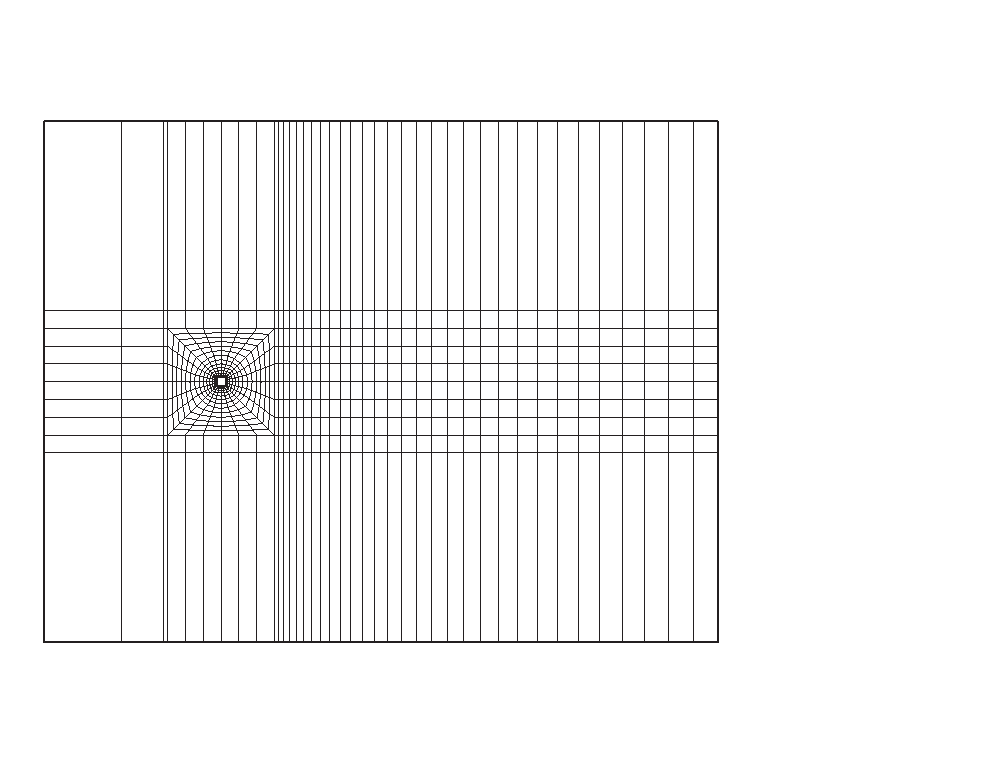
\includegraphics[width=0.8\unitlength]{./chapter-methodology/fnp/square-mesh.eps}}         
      
      
   

      	

  \end{picture}

 \caption{Macro element arrangement in the domain for the square cross section geometry. The inlet extending  $20D$ upstream from the centre of the body, while the outlet extends $60D$ downstream from the centre of the body. The lateral boundaries were placed $20D$ away from the centre of the body.}
    \label{fig:square-mesh}
\end{figure}
 
 
 \begin{figure}
  \setlength{\unitlength}{\textwidth}
\fbox{
  \begin{picture}(0.95,1.3)(0,0.7)
    % % %90
      % % % Parkinson Data 
      \put(0.035,1.65){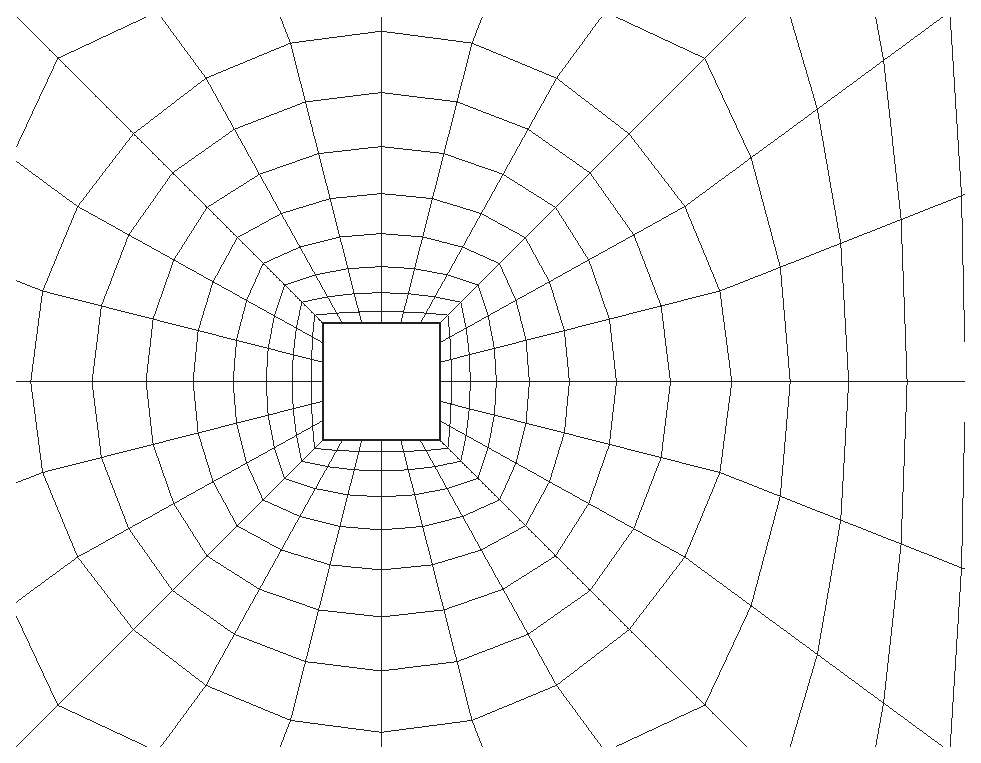
\includegraphics[width=0.4\unitlength]{./chapter-methodology/fnp/mesh.eps}}
      \put(0.495,1.65){\includegraphics[width=0.4\unitlength]{./chapter-methodology/fnp/{hyb0.75-mesh}.eps}}
      \put(0.035,1.25){\includegraphics[width=0.4\unitlength]{./chapter-methodology/fnp/{hyb0.5-mesh}.eps}}
      \put(0.495,1.25){\includegraphics[width=0.4\unitlength]{./chapter-methodology/fnp/{hyb0.25-mesh}.eps}}
      \put(0.3,0.85){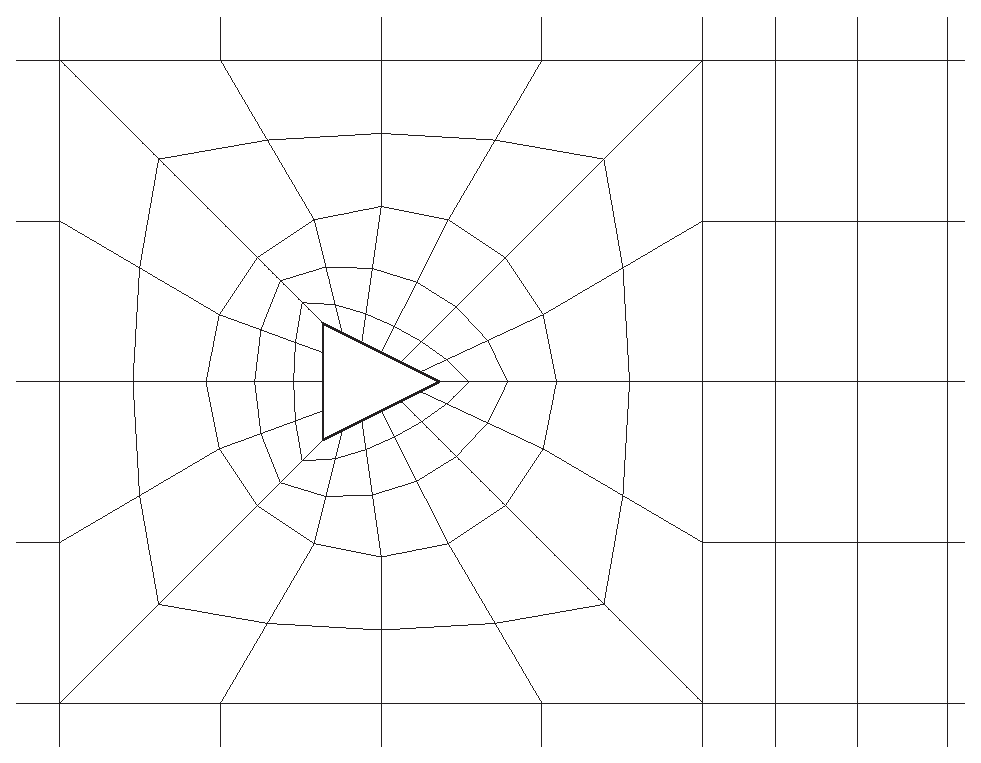
\includegraphics[width=0.4\unitlength]{./chapter-methodology/fnp/triangle-mesh.eps}}
      
      
   
      
      
%      \put(0.23,0.00){ $\displaystyle\frac{c}{\rho\mathcal{A}U}$}
%      \put(0.73,0.00){ $\displaystyle\frac{c}{\rho\mathcal{A}U}$}

     
      \put(0.206,1.605){\small(a)}
      \put(0.665,1.605){\small(b)}
      \put(0.206,1.2){\small(c)}
      \put(0.665,1.2){\small(d)}
      \put(0.45,0.8){\small(e)}
      

  \end{picture}
}
\caption{Configuration of the macro elements near the cross section. (a) square, (b) $\ratio=0.75$, (c) $\ratio=0.5$, (d) $\ratio=0.25$ and (e) triangle.}
  
  \label{fig:zoom-mesh}
\end{figure}

\subsubsection{Convergence}

A series of simulations for the oscillatory cases were carried out in order to ensure the results were grid independent. This was done by keeping the layout of the macro element the same and varying the order of the interpolation polynomial (\emph{p-refinement}). The transverse velocity amplitudes were compared against various polynomial orders. The time step is also reduced as the spectral resolution increases to satisfy the Courant condition. The summary of the results is presented in figure \ref{fig:FSI_convergence} .

% !TeX spellcheck = en_GB
\begin{figure}
  \setlength{\unitlength}{\textwidth}

  \begin{picture}(1,0.3)(-0.02,0)
          
    \put(-0.02,0.04){\includegraphics[width=0.5\unitlength]{./chapter-methodology/fnp/vel-amp-convergencexs.eps}}
    \put(0.5,0.04){\includegraphics[width=0.5\unitlength]{./chapter-methodology/fnp/freq-response-convergencexs.eps}}
        
    \put(0.48,0.166){ $ f_{DNS}$ }
    \put(-0.03,0.166){$\displaystyle\dot{y}_{m}$}
    % \put(0.73,0.00){ $\displaystyle\frac{c}{\rho\mathcal{A}U}$}

    \put(0.23,0.03){\emph{p-order}}
    \put(0.75,0.03){\emph{p-order}}
   
    \put(0.071,0.24){\small(a)}
    \put(0.605,0.24){\small(b)}
      
    \end{picture}

    % \caption{Comparison of DNS data. (a) Maximum power obtained using
    %   a 3 point localised quadratic fitting as a function of
    %   \massstiff. (b) \massdamp as a function of \massstiff at maximum
    %   power}

    \caption{Mean velocity amplitude ($\dot{y}_{m}$) (a) and the galloping frequency ($f_{DNs}$) (b) as a function of the interpolation polynomial. Data present $\frac{tU}{D}=0.001$ (\ding{83}) and $\frac{tU}{D}=0.0005$ ($\bullet$). Data acquired  $\reynoldsnumber=200$ $\massdamp=0$ using FSI direct numerical simulations.}

    \label{fig:FSI_convergence}
\end{figure}

 %vspace{10cm}


Figure \ref{fig:FSI_convergence} shows the mean velocity amplitude (sub-figure (a)) and the galloping frequency (sub-figure (b)) at different polynomial orders. Two factors namely, the quantitative accuracy of the data and the computational time had to be considered during the decision making process to obtain the optimum spacial and temporal resolution. Even though higher order polynomials gave very accurate data, the time step has to be reduced accordingly to meet the Courant condition. As galloping is a low frequency phenomenon, a longer time is taken to achieve the steady oscillating state. Furthermore, as galloping is dependent on the initial excitation of the flow, the initial development of galloping takes a significant amount of time. Both of these factors result in long computation times ranging from 1 to 2 weeks or more. Thus a $9^{th}$ order polynomial was incorporated with $\frac{tU}{D}=0.001$ time-step which produced an acceptable computation time with an acceptable accuracy. A difference of less than $1\%$ was achieved for both mean velocity amplitude  of the body and galloping frequency using these spatial and temporal parameters.

As \citet{Leontini2013}  used an $8^{th}$ order polynomial with a time with a time step of $0.005$, the current study which used a similar mesh as \citet{Leontini2013}, incorporated an $11^{th}$ order polynomial with $\frac{tU}{D}=0.00025$ time-step for static cases, to ensure high accuracy.

As the other cross sections presented in this thesis had relatively small deviation from the original square cross section, the FSI simulations were also carried out using these spatial and temporal parameters.     
















\input{./chapter-methodology/methodology-diff1729e733c018d6203697bd0e55c01828c219fc14.tex}
\chapter{Introduction}

The review of published literature reveals that fluid-elastic galloping has a potential to be used as a mechanism for energy extraction \citep{Barrero-Gil2010a}. Thus, the following questions emerged. What are the optimum parameters for energy transfer in a galloping system? How do they influence galloping?

Another fluid-structure interaction phenomenon, vortex-induced vibration (VIV), has also been investigated as a candidate for the power extraction from flows. The work from \citet{Bernitsas2008a-concept, Bernitsas2009, Raghavan2010a, Lee2011b} and others from the same group at the University of Michigan have made significant progress with this problem. Therefore it may seem, at least initially, reasonable to present data from the fluid-elastic problem in the same parameters as typically used in VIV studies, which could be observed in current literature on galloping \citep{Barrero-Gil2009,Barrero-Gil2010a,Parkinson1964}.



However, the data presented in the pioneering study on energy harvesting from galloping  \citep{Barrero-Gil2010a} presented using classical VIV parameters (i.e. \ustar, $\mstar\zeta$), shows that the mean power data does not collapse well. The reason behind for this hypothesis to be the difference in time-scales of VIV and galloping. Thus the work presented in this chapter is focused on testing this hypothesis and obtain the optimum conditions for mean power output. 

Since the the Quasi-steady state model is the primary mathematical model used to model galloping in this study, the fluid-dynamic characteristics of flow over a static body are presented and discussed first as it is the main input to the QSS model. Then, the natural time scales of the system are obtained using the linearised QSS model. Next, the new non-dimensional governing parameters  \massstiff\ and \massdamp, are formulated by non-dimensionalising the QSS model from these natural time scales. Following this a comparison of galloping data using the classical VIV parameters and  \massstiff\ and \massdamp. Then, the influence of \massstiff \ and \massdamp \ and the conditions for an optimum power output are discussed from QSS data. Finally, the QSS data are compared and discussed against FSI direct numerical simulations and final conclusions are presented.

\clearpage

\subsection{Static body results}

The main data acquisition tool for galloping is the QSS model. As discussed in chapter \ref{sec:QSS_model_methodology},the input to the QSS model is the lift force as a function of the induced angle of attack $\theta$. This function is obtained using lift and drag ($C_y$) data from static body simulations or experiments, to which a polynomial is fitted. These static body data and the polynomial data are presented here in \ref{fig:lift_curves} and \ref{table:cy-coefficients} respectively.  Figure \ref{fig:lift_curves} shows the plots of time averaged $C_y$ data  as a function of $\theta$, as well as the $7^{th}$ order polynomial fits . Data are acquired for high and low Reynolds numbers. For high Reynolds numbers, the static body polynomial data are obtained from \cite{Parkinson1964} while for low Reynolds numbers a $7^{th}$ order non-linear least square regression fit on static body DNS simulations were used. The coefficients of these  polynomials are presented in table \ref{table:cy-coefficients}.


\begin{figure}

  \setlength{\unitlength}{\textwidth}
  \begin{picture}(1,0.25)(0,0.8)
  
    % % %90
      \put(0.025,0.81){\includegraphics[width=0.5\unitlength]{./chapter-pi_1_pi_2/FnP/gnuplot/lift_curve_200.eps}}
      \put(0.495,0.81){\includegraphics[width=0.5\unitlength]{./chapter-pi_1_pi_2/FnP/gnuplot/lift_curve_park.eps}}
 	\put(0.02,0.93){ \large $C_y$} 	
% 	\put(0.56,1.02){ $\theta$}
 	
        \put(0.25,0.8){ $\theta$} 	
        \put(0.75,0.8){ $\theta$}
        
        \put(0.117,1.01){(a)}
        \put(0.565,1.01){(b)}
      \end{picture}

  \caption{Lift coefficient, $C_y$, as a function of incidence angle $\theta$, for a static square cross section. (a) Data from simulations at $Re=200$  (b) data from \cite{Parkinson1964} at $Re=22300$. Points ($\bullet$) are measurements from the simulations. At $\reynoldsnumber=200$. Curves in both plots are 7th-order interpolating polynomials used to predict the fluid forcing for the QSS model. $C_y$ is the force coefficient of the force which occurs normal to the induced velocity.}
    \label{fig:lift_curves}
\end{figure}


\begin{table}[ht]

\begin{center}
\setlength{\unitlength}{\textwidth}

\begin{tabular}{c c c c c} % centered columns (4 columns)
\hline\hline %inserts double horizontal lines
\\[0.2ex]
Case & $a_1$ & $a_3$ & $a_5$ & $a_7$ \\ [0.8ex] % inserts table 
%heading
\hline 
\\[0.8ex]% inserts single horizontal line
Re=200 & 2.32 & 197.8 & 4301.7 & 30311.9 \\[0.8ex]% inserting body of the table
Re=22300 & 2.69 & 168 & 1670 & 59900 \\ [1ex] % [1ex] adds vertical space
\hline %inserts single line
\end{tabular}

\caption{Coefficient values used in the 7th order interpolation polynomial for high ($Re=22300$) and low ($Re=200$) Reynolds numbers. These data are used as input data to calculate the right-hand side of Eq. \ref{final_equation_motion} throughout this study.}
 
\label{table:cy-coefficients} % is used to refer this table in the text
\end{center}
\end{table}



There are several differences that can be observed between high and low Reynolds number data. The peak value of $C_y$ is  significantly lower at $\reynoldsnumber=200$ ($C_y=0.12$ at $5^\circ$) compared to $\reynoldsnumber=22300$ ($C_y=0.57$ at $13^\circ$) . The inflection point present around $8^\circ$ for $\reynoldsnumber=22300$ is not present at $\reynoldsnumber=200$. This agrees with the findings of \cite{Luo2003}. \cite{Luo2003} concluded that hysteresis in the system response occurs due to the inflection point in the $C_y$ curve. Therefore, hysteresis could not be observed at $\reynoldsnumber=200$.

The range of incident flow angles where $C_y$ remains positive is narrow at $\reynoldsnumber=200$ ($0^\circ <\theta \leq$ $7^\circ$) compared to $\reynoldsnumber=22300$ ($0^\circ <\theta \leq 15^\circ$). This positive range sustains galloping, as the power is only transferred from the fluid to the supporting structure within this range of incident angles. This is because the fluid forces are acting in the 
direction of velocity of the body, or in phase with, the oscillating body as demonstrated by equation \ref{eqn:power_alt}. Incident angles beyond this range suppress the galloping as power is transferred in the opposite direction, i.e; from body to fluid. Thus, it is expected that the transferred power at $\reynoldsnumber=200$ to be significantly lower than at $\reynoldsnumber=22300$, because of the relative low values of $C_y$ and the narrow range of positive $C_y$ at $\reynoldsnumber=200$.



\subsection{Formulation of the new dimensionless groups \massstiff \ and \massdamp}
\label{sec:newvar}


The natural time scales of the system can be found by solving for the eigenvalues of the linearised equation of motion (Eq:\ref{final_equation_motion}), namely
\begin{equation}
	\label{eqn:eom_linear}
	m\ddot{y}{+}c\dot{y}{+}ky{=}\frac{1}{2}\rho U^2 \mathcal{A} a_1\left(\frac{\dot{y}}{U}\right),
\end{equation}
which is a simplified version of the equation of motion presented in equation \ref{final_equation_motion} with the polynomial series for the lift force truncated at the linear term.

Combining the $\dot{y}$ terms and solving for eigenvalues gives
\begin{equation}
	\label{eqn:eigs}
	\lambda_{1,2}= -\frac{1}{2}\frac{c-\frac{1}{2}\rho U\mathcal{A}a_1}{m}\pm\frac{1}{2}\sqrt{\left[\frac{c-\frac{1}{2}\rho U\mathcal{A}a_1}{m}\right]^2-4\frac{k}{m}}.
\end{equation}

If it is assumed that the spring is relatively weak, $k\rightarrow 0$, a single non-zero eigenvalue remains. This eigenvalue is
\begin{equation}
	\label{eqn:eigs_nospring}
	\lambda=-\frac{c-\frac{1}{2}\rho U\mathcal{A}a_1}{m}.
\end{equation}

Further, if it is assumed that the mechanical damping is significantly weaker than the fluid-dynamic forces on the body, $c\rightarrow 0$ and
\begin{equation}
	\label{eqn:eigs_nospring_nodamp}
	\lambda=\frac{\frac{1}{2}\rho U\mathcal{A}a_1}{m}.
\end{equation}


In this form, $\lambda$ represents the inverse time scale of the motion of the body due to the effect of the long-time fluid-dynamic forces. In fact, the terms can be regrouped and $\lambda$ written as
\begin{equation}
	\label{eqn:timescale}
	\lambda = \frac{a_1}{m^*}\frac{U}{D}
\end{equation}

Written this way, the important parameters that dictate this inverse time scale are clear. The rate of change in the fluid-dynamic force with respect to angle of attack when the body is at the equilibrium position, $\partial C_y/\partial \alpha$, is represented by $a_1$. The mass ratio is represented by $m^*$. The inverse advective time scale of the incoming flow is represented by the ratio $U/D$. Increasing $a_1$ would mean the force on the body would increase more rapidly with small changes in the angle of attack, $\theta$, or transverse velocity. Equation \ref{eqn:timescale} shows that such a change will increase the inverse time scale, or analogously decrease the response time of the body. Increasing the mass of the body, thereby increasing $m^*$, has the opposite effect. The inverse time scale is decreased, or as might be expected, a heavier body will respond more slowly.

This timescale can then be used to non-dimensionalize the equation of motion, and to find the relevant dimensionless groups of the problem. It was suggested by \citet{shiels2001,leonard2001} to use a flow-based timescale such $D/U$ for the characteristic time for flow-induced vibration problems, rather than a structural-based timescale such as the natural frequency. This point is discussed further in \citet{williamson2004}. Here, this advective time is further scaled by the mass ratio \mstar, as suggested from the eigenvalues of the linearized equation of motion. Hence, if the non-dimensional time, $\tau$, is defined such that $\tau=t(a_1/m^*)(U/D)$, the equation of motion presented in equation \ref{final_equation_motion} can be non-dimensionalized as
\begin{equation}
	\label{eqn:eom_nondim}
	\ddot{Y} + \frac{m^{*2}}{a_1^2}\frac{kD^2}{mU^2}Y = \left(\frac{1}{2} - \frac{m^*}{a_1}\frac{cD}{mU}\right)\dot{Y} - \frac{a_1a_3}{m^{*2}}\dot{Y}^3 + \frac{a_1^3a_5}{m^{*4}}\dot{Y}^5 - \frac{a_1^5a_7}{m^{*6}}\dot{Y}^7.
\end{equation}

The coefficients can be regrouped into combinations of non-dimensional groups, and rewritten as
\begin{equation}
	\label{eqn:eom_nondim_regroup}
	\ddot{Y} + \frac{4\pi^{2}m^{*2}}{U^{*2}a_1^2}Y = \left(\frac{1}{2} - \frac{c^*m^*}{a_1}\right)\dot{Y} - \frac{a_1a_3}{m^{*2}}\dot{Y}^3 + \frac{a_1^3a_5}{m^{*4}}\dot{Y}^5 - \frac{a_1^5a_7}{m^{*6}}\dot{Y}^7,
\end{equation}
where $U^{*}$ is the reduced velocity typically used as an independent variable in vortex-induced vibration studies and $c^*=cD/mU$ is a non-dimensional damping parameter.

Equation \ref{eqn:eom_nondim_regroup} shows there are five non-dimensional parameters that play a role in setting the response of the system. These are the stiffness (represented by the reduced velocity $U^*$), the damping $c^*$, the mass ratio $m^*$, and the geometry and \reynoldsnumber, represented by the coefficients of the polynomial fit to the $C_y$ curve, $a_n$. The grouping of these parameters into two groups in equation \ref{eqn:eom_nondim_regroup} which arise by non-dimensionalising using the natural time scale of the galloping system, suggests there are two groups besides geometry (represented by $a_n$) and \reynoldsnumber that dictate the response: $\Gamma_1 = 4\pi^2m^{*2}/U^{*2}a_1^2$ and $\Gamma_2 = c^*m^*/a_1$. For a given geometry and Reynolds number, $\Gamma_1$ can be thought of as a combined mass-stiffness, whereas $\Gamma_2$ can be thought of a combined mass-damping parameter. It is assumed that during galloping the stiffness plays only a minor role because, galloping time periods are significantly large which implies that $k \rightarrow 0$. Therefore, $\Gamma_2$ seems a likely parameter to collapse the data. In fact, in the classic paper on galloping from \cite{Parkinson1964}, galloping data from wind tunnel tests is presented in terms of a parameter that can be shown to be the same as $\Gamma_2$.

All of the quantities that make up $\Gamma_1$ and $\Gamma_2$ can, in theory, be known before an experiment is conducted. However, the quantity $a_1$ is a relatively difficult one to determine, requiring static body experiments or simulations. Here, the geometry is unchanged and results are only being compared at the same \reynoldsnumber. Hence, suitable parameters can be formed by multiplying $\Gamma_1$ and $\Gamma_2$ by $a_1^2$ and $a_1$ respectively, to arrive at a mass-stiffness parameter $\massstiff =  4\pi^2m^{*2}/U^{*2}$, and a mass-damping parameter defined as $\massdamp = c^*m^*$.

Equation \ref{eqn:eom_nondim_regroup} can be re-written explicitly in terms of \massstiff \ and \massdamp to give

\begin{equation}
	\label{eqn:eom_nondim_regroup_pi_1_pi_2}
	\ddot{Y} + \massstiff Y = \massdamp \dot{Y} - \frac{a_1a_3}{m^{*2}}\dot{Y}^3 + \frac{a_1^3a_5}{m^{*4}}\dot{Y}^5 - \frac{a_1^5a_7}{m^{*6}}\dot{Y}^7.
\end{equation} 

 
 
 \subsection{Comparison of \massstiff \ and \massdamp \ with classical VIV parameters}
 \label{sec:new_vs_viv}
 
 
 Figure \ref{fig:compare_data} shows the comparison of mean power data at $\reynoldsnumber=200$ presented using different independent variables. Subfigures (a), (c) and (e) show the displacement amplitude, velocity amplitude and the mean power as a function of the classic VIV parameter, \ustar \ for various damping ratios $\zeta$. Subfigures (b), (d) and (f) shows the same data as a function of \massdamp, for various, reasonably high values of \massstiff, as defined above in section \ref{sec:newvar}. The data presented using the classical VIV parameters follows the same trends as \cite{Barrero-Gil2010a}. \citet{Barrero-Gil2010a} and \citet{vicente-Ludlam2014} observed that the maximum dimensionless power is achieved at two times the velocity at which the galloping starts. A similar conclusion can be drawn from the data presented here in figures \ref{fig:compare_data}. However, the data presented using the dimensionless group formulated using the natural time scales of the system shows an excellent collapse for both velocity amplitude and mean power, showing that the power is essentially dictated by \massdamp. This implies that unlike VIV which is a type of resonant phenomenon, the natural frequency of the system which is used to scale \ustar, $\zeta$ and \massstiff\ does not have a large influence on the system behaviour in these cases.
 
 \begin{figure}
  \setlength{\unitlength}{\textwidth}
  \fbox{
  \begin{picture}(1,0.9)(0,0)
    % % %90
      % % % Parkinson Data 
      \put(0.035,0.5){\includegraphics[width=0.5\unitlength]{../FnP/gnuplot/displacement_amp_re200.eps}}
      \put(0.035,0.27){\includegraphics[width=0.5\unitlength]{../FnP/gnuplot/velocity_amp_re200.eps}}
      \put(0.035,0.02){\includegraphics[width=0.5\unitlength]{../FnP/gnuplot/mean_power_re_200.eps}}
      
      \put(0.495,0.27){\includegraphics[width=0.5\unitlength]{../FnP/gnuplot/velocity_amp_collapsed_re200.eps}} 
      \put(0.495,0.02){\includegraphics[width=0.5\unitlength]{../FnP/gnuplot/mean_power_collapsed_re_200.eps}}
      \put(0.495,0.5){\includegraphics[width=0.5\unitlength]{../FnP/gnuplot/displacement_amp_collpased_re200.eps}}
      
%      \put(0.23,0.00){ $\displaystyle\frac{c}{\rho\mathcal{A}U}$}
%      \put(0.73,0.00){ $\displaystyle\frac{c}{\rho\mathcal{A}U}$}

      \put(0.28,0.00){\ustar}
      \put(0.78,0.00){\massdamp}
      
      \put(0.01,0.405){$\displaystyle\frac{V}{D}$}\
       \put(0.01,0.63){$\displaystyle\frac{A}{D}$}
      
      \put(-0.02,0.13){$\displaystyle\small\frac{P_{m}}{\rho \mathcal{A}U^3 }$}
      
      \put(0.093,0.705){\small(a)}
      \put(0.555,0.705){\small(b)}
      \put(0.093,0.475){\small(c)}
      \put(0.555,0.475){\small(d)}
      \put(0.093,0.225){\small(e)}
      \put(0.555,0.225){\small(f)}

  \end{picture}
}
  \caption{Displacement amplitude, velocity amplitude and mean power data as functions of two different independent varibles. Data presented in (a), (c) and (e) using the classical VIV parameter $\ustar$, obtained at $Re=200$ and $m^*=20$ at three different damping ratios: $\zeta=0.075$ ($\times$), $\zeta=0.1$ (\ding{117}) and $\zeta=0.15$ (+). (b) (d) and (f)  are the same data presented using the combined mass-damping parameter (\massdamp) as the independent variable.  }
  \label{fig:compare_data}
\end{figure}
 
 \subsection{Comparison of power between high and low \reynoldsnumber\ data}   

\label{sec:low_vs_high_re}
The marked success of the collapse using \massdamp\ for the $\reynoldsnumber = 200$ case, particularly of the mean power, could also be replicated for the higher \reynoldsnumber\ case at $\reynoldsnumber = 22300$. Figure \ref{fig:collapsed_data} presents the mean power for high \reynoldsnumber\ cases for selected values of \massstiff. It is shown that the data collapse in both cases, demonstrating the validity of using \massdamp\ as an independent variable.

% !TeX spellcheck = en_GB
\begin{figure}
  \setlength{\unitlength}{\textwidth}

        \begin{picture}(1,0.3)(-0.02,0)

      % % % Parkinson Data 
%      \put(0.025,0.5){\includegraphics[width=0.5\unitlength]{../FnP/gnuplot/displacement_amp_collapsed_parkinson.eps}}
%      \put(0.025,0.27){\includegraphics[width=0.5\unitlength]{../FnP/gnuplot/velocity_amp_collapsed_parkinson.eps}}
%      \put(0.495,0.27){\includegraphics[width=0.5\unitlength]{../FnP/gnuplot/velocity_amp_collapsed_re200.eps}}
      
      \put(0.025,0.02){\includegraphics[width=0.5\unitlength]{../FnP/gnuplot/mean_power_collapsed_parkinson.eps}}
      \put(0.495,0.02){\includegraphics[width=0.5\unitlength]{../FnP/gnuplot/mean_power_optimum_re_200.eps}}
%      \put(0.495,0.5){\includegraphics[width=0.5\unitlength]{../FnP/gnuplot/displacement_amp_collpased_re200.eps}}
      
%      \put(0.23,0.00){ $\displaystyle\frac{c}{\rho\mathcal{A}U}$}
%      \put(0.73,0.00){ $\displaystyle\frac{c}{\rho\mathcal{A}U}$}

      \put(0.28,0.00){\massdamp}
      \put(0.74,0.00){\massdamp}
      
     
       \put(-0.03,0.13){$\displaystyle\frac{P_{m}}{\rho \mathcal{A}U^3 }$}
      

      \put(0.095,0.218){\small(a)}
      \put(0.565,0.218){\small(b)}
      
    \end{picture}

  \caption{Mean power as a function of \massdamp. Data presented at (a) $\reynoldsnumber=22300$, $\massstiff=200$ ($\times$), $massstiff=2000$ (\ding{117}) and $\massstiff=10000$ (+). (b) $\reynoldsnumber=200$, $\massstiff=100$. Hysteresis could be observed at high \reynoldsnumber  }
    \label{fig:collapsed_data}
\end{figure}

 %vspace{10cm}


Hysteresis could be observed for the $\reynoldsnumber = 22300$ case. The different solutions could be obtained by manipulating the initial conditions (initial displacement) of the system. The upper branch was obtained by giving an initial displacement which was higher than the expected amplitude while the lower branch was obtained by providing a lower initial displacement than the expected amplitude. Although theory shows a possible third state, it is an unstable branch which could not be achieved with a time integration method such as that employed in this study. This was also observed by \cite{Vio2007}.


\subsection{Dependence on mass-stiffness, \massstiff}
\label{subsec:dependence pi_1}

The results of sections \ref{sec:new_vs_viv} and \ref{sec:low_vs_high_re} show that the mean extracted power is essentially a function of a single variable, the combined mass-damping \massdamp. However, the timescale analysis of section \ref{sec:newvar} showed that a second variable, the combined mass-stiffness \massstiff\ should also play a role. Previous studies (see, for example \citet{bouclin:77}) have also indicated a complex interaction between the amplitude and natural frequency, particularly for high natural frequencies (or equivalently, low values of \massstiff). Here, the impact of \massstiff\ is investigated further. Overall, the system behaviour can be separated into two wide regimes; that for ``high'' \massstiff\ and that for ``low'' \massstiff. These two regimes are further investigated and explained in this following section.

Figure \ref{fig:high_pi_1} shows the mean power as a function of \massdamp\ for a range of values of \massstiff. Two subfigures are shown; subfigure (a) shows data for $\massstiff \geq 10$, while (b) shows data for $\massstiff \leq 10$. In figure \ref{fig:high_pi_1}(a), the collapse of the mean power is excellent, showing that for $\massstiff \geq 10$, the mean power is independent of \massstiff.

\begin{figure}
  \setlength{\unitlength}{\textwidth}
\fbox{
        \begin{picture}(1,1.1)(0,0.35)

      % % % Parkinson Data 
      \put(0.09,1.1){\includegraphics[width=0.757\unitlength]{../FnP/gnuplot/displacement_high_pi_1.eps}}
      \put(0.1,0.75){\includegraphics[width=0.75\unitlength]{../FnP/gnuplot/velocity_high_pi_1.eps}}
      \put(0.1,0.35){\includegraphics[width=0.75\unitlength]{../FnP/gnuplot/mean_power_high_pi_1.eps}}
      
         \put(0.07,0.95){$\displaystyle\frac{V}{D}$}\
         \put(0.07,1.3){$\displaystyle\frac{A}{D}$}
         \put(0.05,0.6){$\displaystyle\frac{P_{m}}{\rho \mathcal{A}U^3 }$}



%      
%      \put(0.45,0.7){\small(a)}
%      \put(0.926,0.7){\small(b)}
%      \put(0.726,0.45){\small(c)}
%  

      
    \end{picture}
}
  \caption{QSS data at high \massstiff \ levels. (a) displacement amplitude, (b) velocity amplitude and (c) mean power as a function of \massdamp. Data presented at four different combined mass-stiffness levels.\ $\massstiff=10 \ (\mstar=20,\ \ustar \approx 40)$ \ (\ding{117}),\ $\massstiff=100 \ (\mstar=130,\ \ustar \approx 80) \ (+)$ and \ $\massstiff=1000 \ (\mstar=400,\ \ustar \approx 40) \ (\triangle)$}
    \label{fig:high_pi_1}
\end{figure}

 %vspace{10cm}


For low values of $\massstiff \leq 10$, figure \ref{fig:high_pi_1}(b) shows that the predicted mean power increases as \massstiff\ is decreased, indicating that the mean power is a weak function of \massstiff\ at low \massstiff\ levels. This provides the distinction between high and low \massstiff\ regimes. For high values where $\massstiff \geq 10$, the mean extracted power is a function of \massdamp\ only; for low values where $\massstiff < 10$, the mean extracted power is a weak function of \massstiff.

Regardless of the value of \massstiff, the variation of the mean extracted power with \massdamp\ is essentially the same. With increasing \massdamp, the mean extracted power initially increases, before reaching some maximum value and then decreasing. This relationship between power and \massdamp\ can be explained by analysing the time histories of selected cases. Data at $\massstiff=10$, $m^*=20$ and $\reynoldsnumber=200$ are shown in figure \ref{fig:power_time_histories} and are analysed as an example. Values of \massdamp\ less than (region 1), equal to (region 2), and greater than (region 3) the value where the mean extracted power is a maximum are analysed as examples.

\begin{figure}

  \setlength{\unitlength}{\textwidth}
%  \fbox{
  \begin{picture}(1,0.58)(0,0.35)
    % % % 90
    \put(0.03,0.76){\includegraphics[width=0.35\unitlength]{../FnP/gnuplot/power_time_history_015.eps}}
    \put(0.03,.58){\includegraphics[width=0.35\unitlength]{../FnP/gnuplot/f_y_history_015.eps}}
    \put(0.03,0.4){\includegraphics[width=0.35\unitlength]{../FnP/gnuplot/theta_time_history_015.eps}}
    
    % % 165
    \put(0.36,0.76){\includegraphics[width=0.35\unitlength]{../FnP/gnuplot/power_time_history_54.eps}}
    \put(0.36,.58){\includegraphics[width=0.35\unitlength]{../FnP/gnuplot/f_y_history_54.eps}}
    \put(0.36,0.4){\includegraphics[width=0.35\unitlength]{../FnP/gnuplot/theta_time_history_54.eps}}
    
    \put(0.68,0.76){\includegraphics[width=0.35\unitlength]{../FnP/gnuplot/power_time_history_08.eps}}
    \put(0.68,.58){\includegraphics[width=0.35\unitlength]{../FnP/gnuplot/f_y_history_08.eps}}
    \put(0.68,0.4){\includegraphics[width=0.35\unitlength]{../FnP/gnuplot/theta_time_history_08.eps}}
    
    \put(0.55,0.36){$\displaystyle{\frac{tU}{D}}$}
    \put(0.2,0.36){$\displaystyle{\frac{tU}{D}}$}
    \put(0.85,0.36){$\displaystyle{\frac{tU}{D}}$}
    
    \put(0.0,0.87){$\frac{P}{\rho \mathcal{A}U^3}$}
    \put(0.01,0.66){$F_y$}
    \put(0.01,0.49){$\theta$}
    
    \put(0.08,0.76){(a)}
    \put(0.08,0.58){(d)}
    \put(0.08,0.38){(g)}
    
    \put(0.4,0.76){(b)}
    \put(0.4,0.58){(e)}
    \put(0.4,0.38){(h)}
    
    \put(0.72,0.76){(c)}
    \put(0.72,0.58){(f)}
    \put(0.72,0.38){(i)}
  \end{picture}
%}
  \caption{Time histories of $P_t$, $P_d$, $F_y$ and $\theta$ at $\massdamp=0.15$, $0.54$ and $0.8$ from the QSS model. Data was obtained at $m^*=20$, $\massstiff=10$ and \reynoldsnumber=200. The time histories of $P_t$ ( \solidrule[4mm]\hspace{1mm}) and $P_d$ (\protect\dashedrule) are presented for: (a) $\massdamp= 0.15$; (b) $\massdamp= 0.54$; (c) $\massdamp= 0.8$. Time histories of the instantaneous force $F_y$ for: (d) $\massdamp= 0.15$; (e) $\massdamp= 0.54$; (f) $\massdamp= 0.8$. Time histories of the instantaneous angle $\theta$ for: (g) $\massdamp= 0.15$; (h) $\massdamp= 0.55$; (i) $\massdamp= 0.8$.}
  \label{fig:power_time_histories}
\end{figure}






The instantaneous power from the fluid to the body can be expressed as $P_t=F_y\dot{y}$. Similarly the dissipated power due to the mechanical damping can be expressed as $P_d=(c\dot{y})\dot{y}$. The time average of these two quantities, described in equations \ref{eqn:power} and \ref{eqn:power_alt} must be equal due to energy conservation.

% Figure \ref{fig:lift_curves}(a) shows that $C_y$ and therefore instantaneous force rises until $4^\circ$ where it peaks and then falls, and at around $6^\circ$ becomes negative. The maximum instantaneous power that can be transferred occurs when $C_t\dot{y}$ is a maximum which occurs when $\theta$ is close to the peak in the $C_y$  curve . At the region where the instantaneous force becomes negative it will be opposing the velocity $\dot{y}$. 

% % % % % % % % % % % don  

At region 1 ($\massdamp=0.15$) the damping is low in comparison with region 2 and 3. While this may lead to larger oscillations, damping is required to dissipate and therefore extract power according to equation \ref{eqn:power}. Therefore, the low damping in this region leads to a low mean power output. Fig.\ref{fig:power_time_histories} (a) shows that $P_d$ (the power dissipated by damping) becomes negative over some portion of the cycle. This is caused by the high velocity amplitude leading to the equivalent incident angle $\theta$ to exceed the range where $C_y$ is positive (i.e. $0<\theta<6^\circ$ as shown in figure\ref{cy ploynomial}(a)). In this portion of the cycle the fluid-dynamic force actually opposes the direction of travel and power is transferred from the structure to the fluid during those times. From an energy perspective, the mechanical damping is not sufficient to remove the energy transferred from the fluid to the structure through work during other times of the cycle because $\massdamp$ \ is substantially low. Therefore this excess energy is transferred back to the fluid as depicted by the negative region of $P_d$.

\vspace{1mm} 
At region 3 where $\massdamp=0.8$ the damping constant is high and a clear sinusoidal signal is observed for both $P_d$ and $P_t$ in figure \ref{fig:power_time_histories}(c). Figures \ref{fig:power_time_histories}(f) and  \ref{fig:power_time_histories}(i) show that equivalent incident angle $\theta$ (which for small values, is proportional to the transverse velocity of the body) is in phase with $F_y$.  The velocity amplitude in this case is small and $\theta$ is within the range where the fluid-dynamic force increases with the incident angle (i.e. $0<\theta \leq 5^\circ$ as shown in figure \ref{fig:lift_curves}(a)). According to equation \ref{eqn:power_alt}, these conditions are suitable for high power output. However in this case, the high damping limits the velocity amplitude and results in relatively low fluid dynamic forces.

At region 2 ( $\massdamp=0.54$), a balance is found between high and low values of damping. $P_d$ is not a pure sinusoidal signal, however the signal remains periodic. From the time history graph of $P_d$, two `peaks' are present in a single half cycle as shown in figure \ref{fig:power_time_histories}(b). In this case, the velocity amplitude actually exceeds the equivalent incident angle where the fluid-dynamic forces peaks (i.e. $\theta=5^\circ$ in \ref{cy ploynomial} (a)). The dips in $P_d$ between the two peaks approximately correspond to the time where the transverse velocity is higher than 0.09 and $F_y$ is decreasing with increasing transverse velocity. The mean power output is at its maximum. This is due to the fact that this region is the best compromise between region 1 and 3. The damping is high enough to obtain a high power output while not so high that the motion is completely suppressed.


\subsection{Dependence on the mass ratio \mstar}
\label{sec:mstar}
While for high values of \massstiff\ it is clear that the mean extracted power is a function of \massdamp\ only, a question arises for low values of \massstiff; is the variation in the mean extracted power purely a function of \massstiff, or is it also a function of the mass ratio \mstar? To answer this question, the model has been solved for a fixed value of \massstiff, but for varying values of \mstar. This means that \massstiff\ was varied by changing the system stiffness.

Figure \ref{fig:low_pi_1} shows the mean extracted power as a function of \massdamp, for a fixed $\massstiff = 0.1$, for three different values of \mstar. From the figure it is clear that the results are independent of \mstar, and are a function of \massstiff\ and \massdamp\ only.

\begin{figure}
  \setlength{\unitlength}{\textwidth}

        \begin{picture}(1,0.4)(0,0.4)

      % % % Parkinson Data 
%      \put(0.1,1.1){\includegraphics[width=0.75\unitlength]{../FnP/gnuplot/displacement_low_pi_1.eps}}
%      \put(0.1,0.76){\includegraphics[width=0.75\unitlength]{../FnP/gnuplot/velocity_low_pi_1.eps}}
      \put(0.1,0.42){\includegraphics[width=0.75\unitlength]{./chapter-pi_1_pi_2/FnP/gnuplot/mean_power_low_pi_1.eps}}
      
%       \put(0.07,0.95){$\displaystyle\frac{V}{D}$}
%       \put(0.07,1.3){$\displaystyle\frac{A}{D}$}
       \put(0.05,0.6){$\displaystyle\frac{P_{m}}{\rho \mathcal{A}U^3 }$}
       \put(0.5,0.4){$\massdamp$}
       \
%\put(0.189,1.415){\small(a)}
%\put(0.189,1.07){\small(b)}
%\put(0.189,0.73){\small(c)}

%  

      
    \end{picture}

  \caption{Dimensionless mean power as a function of \massdamp\ obtained using QSS model at \ $\massstiff=0.1$.  Data presented at  $\mstar=2$ (\ding{117}), \  $ \mstar=20 \ (\triangle)$ and  $ \mstar=50 \ (*)$. The mass ratio does not have an effect on \massstiff \ even at low \massstiff.}
    \label{fig:low_pi_1}
\end{figure}

 %vspace{10cm}


\subsection{Comparison with DNS data}
\label{sec:dns}

The QSS model assumes that the only force driving the system is the instantaneous lift generated by the induced velocity. However, vortex shedding is also present in this system. Therefore, an essential assumption when this model is used, is that the effect of vortex shedding is minimal. Hence, the model has been always used at high \reynoldsnumber \ and  at high mass ratios. This study is focused on identifying the limiting parameters of the QSS model at low Reynolds numbers by providing a comparison with DNS results. 

\citet{Joly2012} showed that the displacement data obtained using the QSS assumption and DNS agree well at low Reynolds numbers, with the modification implemented to the oscillator equation which accounts for the vortex shedding. These data were obtained at zero damping levels. However, the current study is focused on the behaviour and the power transfer of the system. Therefore analysing the behaviour of the system with increasing damping is of interest.

The comparison between QSS and the DNS results is presented in figure \ref{fig:qss_fsi}. The maximum displacement, velocity and mean extracted power are presented as a function of \massdamp. A range of values of \massstiff\ are compared to the QSS model data for $\massstiff = 10$. Figures \ref{fig:qss_fsi}(a) and \ref{fig:qss_fsi}(b) show little variation with \massstiff, and the comparison between the QSS model and the DNS simulations is quite good. However, the mean extracted power shown in figure \ref{fig:qss_fsi}(c) reveals that the mean power is influenced by both \massstiff\ and \massdamp. This is particularly clear for low values of \massstiff, where the discrepancy between the QSS model predictions of power and the DNS simulations is the largest. Comparing figure \ref{fig:qss_fsi}(c) with figure \ref{fig:high_pi_1}(a) shows that \massstiff\ has much more influence on the power extracted than predicted by the QSS model for low \massstiff \ values. In fact, the QSS model predicts that the mean extracted power should increase with decreasing \massstiff\ when \massstiff\ moves to the low \massstiff\ region (figure \ref{fig:high_pi_1}(b)), whereas the DNS simulations show that the mean extracted power decreases with decreasing \massstiff.

\begin{figure}
  \setlength{\unitlength}{\textwidth}

        \begin{picture}(1,1.1)(0,0.35)

      % % % Parkinson Data 
      \put(0.1,1.1){\includegraphics[width=0.75\unitlength]{./chapter-pi_1_pi_2/FnP/gnuplot/fqss_fsi_displace.eps}}
      \put(0.1,0.737){\includegraphics[width=0.75\unitlength]{./chapter-pi_1_pi_2/FnP/gnuplot/qss_fsi_velocity.eps}}
      \put(0.1,0.38){\includegraphics[width=0.75\unitlength]{./chapter-pi_1_pi_2/FnP/gnuplot/qss_fsi_power.eps}}
      
      



%      
    \put(0.15,1.41){\small(a)}
     \put(0.15,1.05){\small(b)}
     \put(0.15,0.69){\small(c)}
\put(0.03,0.95){$\displaystyle\frac{V}{U}$}
\put(0.03,1.3){$\displaystyle\frac{A}{D}$}
\put(0.0,0.56){$\displaystyle\frac{P_{m}}{\rho \mathcal{A}U^3 }$}
\put(0.466,0.35){$\massdamp$}

      
    \end{picture}

    \caption{Comparison of data generated using the quasi-static model
      and full DNS simulations at (a) Displacement amplitude, (b)
      velocity amplitude and (c) dimensionless mean power as functions of
      \massdamp. Data were obtained at $\reynoldsnumber = 200$ at four
      values $\massstiff=10$ ($\mstar= 20.13$) (\ding{83}),
      $\massstiff=60$ ($\mstar =49.31$) (\ding{108}), $\massstiff=250$
      ($\mstar= 100.7$) ($\triangle$) and $\massstiff=1000$ ($\mstar=201.3$) (\ding{117}). The QSS data at $\massstiff=10$ \
      (\protect\dashedrule).}
    \label{fig:qss_fsi}
\end{figure}

 %vspace{10cm}


Figure \ref{fig:max_power}(a) clearly shows the dependence of the mean extracted power on \massstiff. Here, the maximum power extracted for a given value of \massstiff, over all values of \massdamp (essentially the value of extracted power at the turning point), is plotted as a function of \massstiff. These values were obtained by fitting a quadratic to the data of figure \ref{fig:low_pi_1} and finding the value of mean extracted power at the turning point. The rapid decrease in the extracted power as $\massstiff \rightarrow 0$ is clear.

% !TeX spellcheck = en_GB
\begin{figure}
  \setlength{\unitlength}{\textwidth}
  \begin{picture}(1,0.3)(-0.02,0)
          
    \put(0.025,0.04){\includegraphics[width=0.45\unitlength]{../FnP/gnuplot/p_max.eps}}
    \put(0.54,0.04){\includegraphics[width=0.45\unitlength]{../FnP/gnuplot/p_2_p_max.eps}}
        
    \put(0.48,0.07){ \rotatebox{90}{$\displaystyle\massdamp$ \scriptsize{at max power}} }
    \put(-0.07,0.16){$\displaystyle\frac{P_{max}}{\rho \mathcal{A}U^3 }$}
    % \put(0.73,0.00){ $\displaystyle\frac{c}{\rho\mathcal{A}U}$}

    \put(0.24,0.00){\massstiff}
    \put(0.75,0.00){\massstiff}
   
    \put(0.058,0.07){\small(a)}
    \put(0.57,0.07){\small(b)}
      
    \end{picture}

    % \caption{Comparison of DNS data. (a) Maximum power obtained using
    %   a 3 point localised quadratic fitting as a function of
    %   \massstiff. (b) \massdamp as a function of \massstiff at maximum
    %   power}

    \caption{(a) Maximum power of QSS data ($\circ$) and DNS data ($\bullet$), and (b) the value of \massdamp\ 
        where maximum power occurs in DNS data, as functions of \massstiff.
           The maximum power asymptotes to an upper
        value with increasing \massstiff, while the value of \massdamp\
        where maximum power occurs is relatively insensitive to
        \massstiff. The maximum power of the DNS data remains relatively constant as shown before. The dash curve (\protect\dashedrule) of (a) follows the logarithmic fit of the maximum power which is $f(x)=1.48 \times 10^{-4} \ ln(x) + 1.9 \times 10^{-3} $ equation.}

    \label{fig:max_power}
\end{figure}

 %vspace{10cm}


Figure \ref{fig:max_power}(a) also shows that \massstiff\ is important to higher values than predicted by the QSS model. For the QSS model, the mean extracted power was essentially independent of \massstiff\ for $\massstiff>10$, as shown by the open symbols on the figure. However, the mean extracted power from the DNS data shows a significant dependence on \massstiff\ for $\massstiff<250$. Even so, the power extracted during the DNS simulations converges to the value predicted by the QSS model as \massstiff\ increases.

Figure \ref{fig:max_power}(b) shows the value of \massdamp\ at which the turning point, and therefore the maximum power output, occurs. The open symbols show the value predicted by the QSS model, the closed symbols show the value predicted by the DNS. The two are not the same, with a value around $0.41$ predicted by the DNS (shown with a dashed line) and a value above $0.5$ predicted by the QSS model. However, both models show that while the power extracted is a reasonably strong function of \massstiff, the value of \massdamp\ at which this maximum power occurs is relatively unaffected.

In an effort to further quantify the performance of the QSS model, the percentage between the QSS and DNS extracted power data as a function of \massstiff\ was calculated using the equation
\begin{equation}   \label{eqn:error_calculation} 
\% \ error=\left|{\frac{P_{m(QSS)} - P_{m(DNS)}}{P_{m(DNS)}}}\right| \times 100.
\end{equation}

The results of this calculation are plotted in figure \ref{fig:error}, along with a power-law best fit $138.697\massstiff^{-0.6}$. The figure clearly shows that as \massstiff \ increases, the error between the QSS and DNS models quickly decreases. However, at low values of \massstiff, the discrepancy between the two can be quite large, around $30\%$.

\begin{figure}
  \setlength{\unitlength}{\textwidth}

        \begin{picture}(1,0.4)(0,0.4)

      \put(0.1,0.45){\includegraphics[width=0.75\unitlength]{../FnP/gnuplot/error.eps}}
      
%       \put(0.07,0.95){$\displaystyle\frac{V}{D}$}
%       \put(0.07,1.3){$\displaystyle\frac{A}{D}$}
       \put(0.05,0.58){\rotatebox{90}{$\% \ error$}}
%       \put(0.5,0.4){$\massdamp$}
       \put(0.5,0.4){$\massstiff$}
    \end{picture}

  % \caption{Comparison of maximum power between QSS and DNS data obtained using 3 point local quadratic curve fitting.The error was obtained using Eq:\ref{eqn:error_calculation}}
    \caption{The difference between the maximum power predicted by
        the QSS model for $\massstiff = 10$, and the DNS data as a
        function of \massstiff. The QSS model prediction is worst for
        low values of \massstiff.}
    \label{fig:error}
\end{figure}

 %vspace{10cm}


A likely reason for this discrepancy at low \massstiff\ is the influence of the vortex shedding, which is not accounted for in the QSS model. To investigate this further, frequency spectra for the body velocity from DNS cases at varying values of \massstiff, at a value of $\massdamp=0.47$ (close to the value at which the mean extracted power is a maximum), have been produced. They are presented, along with the original time histories in figure \ref{fig:spectrum}.

\begin{figure}
  \setlength{\unitlength}{\textwidth}

  \begin{picture}(1,1.2)(0,-0.1)
    % % %90
      % % % Parkinson Data 
      \put(0.005,0.8){\includegraphics[width=0.5\unitlength]{../FnP/gnuplot/spec_20_sig.eps}}
      \put(0.005,0.5){\includegraphics[width=0.5\unitlength]{../FnP/gnuplot/spec_50_sig.eps}}
      \put(0.005,0.27){\includegraphics[width=0.5\unitlength]{../FnP/gnuplot/spec_100_sig.eps}}
      \put(0.005,0.02){\includegraphics[width=0.5\unitlength]{../FnP/gnuplot/spec_200_sig.eps}}
      
      
      \put(0.505,0.8){\includegraphics[width=0.5\unitlength]{../FnP/gnuplot/spec_20.eps}}
      \put(0.505,0.5){\includegraphics[width=0.5\unitlength]{../FnP/gnuplot/spec_50.eps}}
      \put(0.505,0.27){\includegraphics[width=0.5\unitlength]{../FnP/gnuplot/spec_100.eps}} 
      \put(0.505,0.02){\includegraphics[width=0.5\unitlength]{../FnP/gnuplot/spec_200.eps}}
      
      
%      \put(0.23,0.00){ $\displaystyle\frac{c}{\rho\mathcal{A}U}$}
%      \put(0.73,0.00){ $\displaystyle\frac{c}{\rho\mathcal{A}U}$}

      \put(0.28,-0.03){$\displaystyle\frac{fd}{U}$}
      \put(0.78,-0.03){$\displaystyle\frac{tU}{D}$}
      
      \put(0.51,0.405){$\displaystyle\frac{V}{D}$}
      \put(0.51,0.63){$\displaystyle\frac{V}{D}$}
      \put(0.51,0.13){$\displaystyle\frac{V}{D}$}
      \put(0.51,0.93){$\displaystyle\frac{V}{D}$}
      
      \put(0.10,0.995){\small(a)}
      \put(0.625,0.995){\small(b)}
      \put(0.1,0.695){\small(c)}
      \put(0.625,0.695){\small(d)}
      \put(0.1,0.465){\small(e)}
      \put(0.625,0.465){\small(f)}
      \put(0.1,0.217){\small(g)}
      \put(0.625,0.217){\small(h)}

  \end{picture}

  \caption{Velocity signal (right) and the corresponding power spectrum (left) of the DNS data at 3 different \massstiff \ at $\massdamp=0.8$. (a) and (b) $\massstiff=10$, (c) and (d) $\massstiff=60$, (e) and (f) $\massstiff=250$, (g) and (h) $\massstiff=1000$. \ustar \ is kept at 40 therefore the mass ratio increases as \ \massstiff \ increases. It is evident that the influence of vortex shedding reduces as the inertia of the system increases.}
  \label{fig:spectrum}
\end{figure}

This figure shows the  velocity signals at $\massstiff=0.8$ and $\massdamp= 10, 60, 250$ and $1000$ and the corresponding spectrum. The spectral data shows a significant frequency component around $fd/U=0.156$ which can be identified as the vortex shedding frequency. The magnitude of the frequency component at the vortex shedding frequency clearly reduces as \massstiff\ is increased. This indicates that the influence of vortex shedding is much more prominent at low \massstiff,  therefore resulting in larger deviations from quasi-steady state results. This builds on the work of \cite{Joly2012}, which was conducted at zero damping, that implied that mean extracted power would be influenced by vortex shedding at low mass.

This influence is explicitly shown here. Figure \ref{fig:spec_pow} plots the relative intensity of the component at the vortex shedding frequency to the component at the galloping or oscillation frequency in the spectra of figure \ref{fig:spectrum}.

\begin{figure}
  \setlength{\unitlength}{\textwidth}

        \begin{picture}(1,0.4)(0,0.4)

      \put(0.1,0.45){\includegraphics[width=0.75\unitlength]{../FnP/gnuplot/spec_pow.eps}}
      
%       \put(0.07,0.95){$\displaystyle\frac{V}{D}$}
%       \put(0.07,1.3){$\displaystyle\frac{A}{D}$}
       \put(0.045,0.43){\rotatebox{90}{$relative \ power \ of \ shedding$ }}
%       \put(0.5,0.4){$\massdamp$}
       \put(0.43,0.4){$\massstiff$}
    \end{picture}

  % \caption{Comparison of maximum power between QSS and DNS data obtained using 3 point local quadratic curve fitting.The error was obtained using Eq:\ref{eqn:error_calculation}}
    \caption{The relative power of the vortex shedding as a fucntion of \massstiff. The relative power of the vortex shedding decreases as \massstiff \ increases. This trend follows $0.977x^{-0.5}$ equation}
    \label{fig:spec_pow}
\end{figure}

 %vspace{10cm}



Similar to the discrepancy between the QSS and DNS mean extracted power shown in figure \ref{fig:error}, the relative strength of the vortex shedding is seen to be large at small values of \massstiff, and quickly decreases as \massstiff\ is increased. The figure shows that the relative power of the vortex shedding frequency to the galloping frequency varies like $0.977\massstiff^{-0.52}$.

The difference between the power predicted by the QSS and DNS models scales with $\massstiff^{-0.6}$; the relative power at the vortex shedding frequency scales with $\massstiff^{-0.52}$. These scalings are quite similar, and both are close to $1/\sqrt{\massstiff}$. While not unequivocal, this correlation strongly indicates this discrepancy is due to the influence of the vortex shedding, even though the vortex shedding and galloping frequencies remain separated by around the same amount for all values of \massstiff\ presented in figure \ref{fig:spectrum}. The data presented in figure \ref{fig:spec_pow} also give some indication of the strength of any vortex shedding correction term that might be added to the QSS model in an effort to decrease the discrepancy between it and the DNS simulations.

\begin{figure} [!htb]
  \setlength{\unitlength}{\textwidth}
  \begin{picture}(1,1.1)(0,0.66)
    
    \put(0,1.5){\includegraphics[width=1\unitlength]{../FnP/gnuplot/10.eps}}
    \put(0,1.22){\includegraphics[width=1\unitlength]{../FnP/gnuplot/60.eps}}
    \put(0,0.94){\includegraphics[width=1\unitlength]{../FnP/gnuplot/250.eps}}
    \put(0,0.66){\includegraphics[width=1\unitlength]{../FnP/gnuplot/1000.eps}}

    \put(0.01,1.72){\small(a)}
    \put(0.01,1.44){\small(b)}
    \put(0.01,1.16){\small(c)}
    \put(0.01,0.88){\small(d)}
      
  \end{picture}

  \caption{Vorticity plots of the flow at arbitrary instants at
    $\massdamp=0.47$. (a) $\massstiff=10$, (b) $\massstiff=60$ (c)
    $\massstiff=250$ and (d) $\massstiff=1000$ at
    $\reynoldsnumber=200$. Contours show vorticity at levels between
    $\pm 1$.}
    \label{fig:flow_vis}
\end{figure}

 %vspace{10cm}


Further information can be gained by observing the flow field. Non-dimensionalised flow field data at values of \massdamp\ close to where maximum power is produced at different \massstiff\ are presented in figure \ref{fig:flow_vis}. The figure shows a clear wavelength of the wake as \massstiff \ is increased. Qualitatively, this can be interpreted as showing that at high \massstiff, the vortex shedding is simply superimposed over the path of motion of the cylinder. It shows a decrease in amplitude of the path of the body at low \massstiff, which may be due to the higher levels of non-linear interaction between the vortex shedding and galloping. Such an argument is consistent with the data of figure \ref{fig:spec_pow} that show the increasing influence of vortex shedding on the velocity of the body as \massstiff\ decreases. Taken together, this also goes some way to explaining the discrepancy between the output power predicted by the QSS and DNS models at low \massstiff, highlighted in figure \ref{fig:error}.


\section{Summary of the governing parameters of  fluid-elastic galloping}
\label{sec:summary-pi_1-pi_2}

A need arose after the literature survey to obtain suitable scaling parameters for galloping. These parameters \massstiff\ and \massdamp, were formulated through the natural time-scales of the linearised Quasi-steady state model.   

The power transfer of a square body under fluid-elastic galloping was analysed by solving the quasi-steady state oscillator model equation using numerical  integration. Power data were analysed for both traditional VIV and the newly formulated scaling parameters.A good collapse for predicted output of power could be obtained using the newly formulated  dimensionless groups (\massstiff, \massdamp) in comparison with the classical VIV parameters ,i.e., $\zeta$ and \ustar. The collapsed data using the dimensionless groups strengthens the argument that the velocity amplitude and the power transfer of the system does not depend on the natural frequency of the system over a large range of natural frequencies.

Even though \mstar is an independent parameter as shown in equation \ref{eqn:eom_nondim_regroup_pi_1_pi_2}, the results showed that the system is essentially a function of \massstiff\ and \massdamp\ only.  This seems to be explained by inspection of  equation \ref{eqn:eom_nondim_regroup_pi_1_pi_2}, which shows that \mstar only has an impact on the forcing terms which are non-linear in relation to the body velocity. For these terms to be appreciable, the velocity of the body (and therefore the induced angle of attack) needs to be very high, which appears not to be the case for the range of parameters tested here. 

In comparison with the direct numerical simulation data, it could be concluded that the QSS model provides a good estimate of the power output of the system when \massstiff\ is relatively high. However, at low values of \massstiff, the prediction is not close due to the fact that the QSS model does not account for the influence of vortex shedding which is shown to increase as \massstiff\ is decreased. However, the QSS model does provide a reasonable prediction of the value of \massdamp\ at which maximum power is produced. Both the error in predicted maximum power between the QSS and the DNS models, and the relative power of the vortex shedding, have been quantified and scale similarly to $1/\sqrt{\massstiff}$.

 










<<<<<<< HEAD
\chapter{Introduction}

The review of published literature reveals that fluid-elastic galloping has a potential to be used as a mechanism for energy extraction \citep{Barrero-Gil2010a}. Thus, the following questions emerged. What are the optimum parameters for energy transfer in a galloping system? How do they influence galloping?

Another fluid-structure interaction phenomenon, vortex-induced vibration (VIV), has also been investigated as a candidate for the power extraction from flows. The work from \citet{Bernitsas2008a-concept, Bernitsas2009, Raghavan2010a, Lee2011b} and others from the same group at the University of Michigan have made significant progress with this problem. Therefore it may seem, at least initially, reasonable to present data from the fluid-elastic problem in the same parameters as typically used in VIV studies, which could be observed in current literature on galloping \citep{Barrero-Gil2009,Barrero-Gil2010a,Parkinson1964}.



However, the data presented in the pioneering study on energy harvesting from galloping  \citep{Barrero-Gil2010a} presented using classical VIV parameters (i.e. \ustar, $\mstar\zeta$), shows that the mean power data does not collapse well. The reason behind for this hypothesis to be the difference in time-scales of VIV and galloping. Thus the work presented in this chapter is focused on testing this hypothesis and obtain the optimum conditions for mean power output. 

Since the the Quasi-steady state model is the primary mathematical model used to model galloping in this study, the fluid-dynamic characteristics of flow over a static body are presented and discussed first as it is the main input to the QSS model. Then, the natural time scales of the system are obtained using the linearised QSS model. Next, the new non-dimensional governing parameters  \massstiff\ and \massdamp, are formulated by non-dimensionalising the QSS model from these natural time scales. Following this a comparison of galloping data using the classical VIV parameters and  \massstiff\ and \massdamp. Then, the influence of \massstiff \ and \massdamp \ and the conditions for an optimum power output are discussed from QSS data. Finally, the QSS data are compared and discussed against FSI direct numerical simulations and final conclusions are presented.

\clearpage

\subsection{Static body results}

The main data acquisition tool for galloping is the QSS model. As discussed in chapter \ref{sec:QSS_model_methodology},the input to the QSS model is the lift force as a function of the induced angle of attack $\theta$. This function is obtained using lift and drag ($C_y$) data from static body simulations or experiments, to which a polynomial is fitted. These static body data and the polynomial data are presented here in \ref{fig:lift_curves} and \ref{table:cy-coefficients} respectively.  Figure \ref{fig:lift_curves} shows the plots of time averaged $C_y$ data  as a function of $\theta$, as well as the $7^{th}$ order polynomial fits . Data are acquired for high and low Reynolds numbers. For high Reynolds numbers, the static body polynomial data are obtained from \cite{Parkinson1964} while for low Reynolds numbers a $7^{th}$ order non-linear least square regression fit on static body DNS simulations were used. The coefficients of these  polynomials are presented in table \ref{table:cy-coefficients}.


\begin{figure}

  \setlength{\unitlength}{\textwidth}
  \begin{picture}(1,0.25)(0,0.8)
  
    % % %90
      \put(0.025,0.81){\includegraphics[width=0.5\unitlength]{./chapter-pi_1_pi_2/FnP/gnuplot/lift_curve_200.eps}}
      \put(0.495,0.81){\includegraphics[width=0.5\unitlength]{./chapter-pi_1_pi_2/FnP/gnuplot/lift_curve_park.eps}}
 	\put(0.02,0.93){ \large $C_y$} 	
% 	\put(0.56,1.02){ $\theta$}
 	
        \put(0.25,0.8){ $\theta$} 	
        \put(0.75,0.8){ $\theta$}
        
        \put(0.117,1.01){(a)}
        \put(0.565,1.01){(b)}
      \end{picture}

  \caption{Lift coefficient, $C_y$, as a function of incidence angle $\theta$, for a static square cross section. (a) Data from simulations at $Re=200$  (b) data from \cite{Parkinson1964} at $Re=22300$. Points ($\bullet$) are measurements from the simulations. At $\reynoldsnumber=200$. Curves in both plots are 7th-order interpolating polynomials used to predict the fluid forcing for the QSS model. $C_y$ is the force coefficient of the force which occurs normal to the induced velocity.}
    \label{fig:lift_curves}
\end{figure}


\begin{table}[ht]

\begin{center}
\setlength{\unitlength}{\textwidth}

\begin{tabular}{c c c c c} % centered columns (4 columns)
\hline\hline %inserts double horizontal lines
\\[0.2ex]
Case & $a_1$ & $a_3$ & $a_5$ & $a_7$ \\ [0.8ex] % inserts table 
%heading
\hline 
\\[0.8ex]% inserts single horizontal line
Re=200 & 2.32 & 197.8 & 4301.7 & 30311.9 \\[0.8ex]% inserting body of the table
Re=22300 & 2.69 & 168 & 1670 & 59900 \\ [1ex] % [1ex] adds vertical space
\hline %inserts single line
\end{tabular}

\caption{Coefficient values used in the 7th order interpolation polynomial for high ($Re=22300$) and low ($Re=200$) Reynolds numbers. These data are used as input data to calculate the right-hand side of Eq. \ref{final_equation_motion} throughout this study.}
 
\label{table:cy-coefficients} % is used to refer this table in the text
\end{center}
\end{table}



There are several differences that can be observed between high and low Reynolds number data. The peak value of $C_y$ is  significantly lower at $\reynoldsnumber=200$ ($C_y=0.12$ at $5^\circ$) compared to $\reynoldsnumber=22300$ ($C_y=0.57$ at $13^\circ$) . The inflection point present around $8^\circ$ for $\reynoldsnumber=22300$ is not present at $\reynoldsnumber=200$. This agrees with the findings of \cite{Luo2003}. \cite{Luo2003} concluded that hysteresis in the system response occurs due to the inflection point in the $C_y$ curve. Therefore, hysteresis could not be observed at $\reynoldsnumber=200$.

The range of incident flow angles where $C_y$ remains positive is narrow at $\reynoldsnumber=200$ ($0^\circ <\theta \leq$ $7^\circ$) compared to $\reynoldsnumber=22300$ ($0^\circ <\theta \leq 15^\circ$). This positive range sustains galloping, as the power is only transferred from the fluid to the supporting structure within this range of incident angles. This is because the fluid forces are acting in the 
direction of velocity of the body, or in phase with, the oscillating body as demonstrated by equation \ref{eqn:power_alt}. Incident angles beyond this range suppress the galloping as power is transferred in the opposite direction, i.e; from body to fluid. Thus, it is expected that the transferred power at $\reynoldsnumber=200$ to be significantly lower than at $\reynoldsnumber=22300$, because of the relative low values of $C_y$ and the narrow range of positive $C_y$ at $\reynoldsnumber=200$.



\subsection{Formulation of the new dimensionless groups \massstiff \ and \massdamp}
\label{sec:newvar}


The natural time scales of the system can be found by solving for the eigenvalues of the linearised equation of motion (Eq:\ref{final_equation_motion}), namely
\begin{equation}
	\label{eqn:eom_linear}
	m\ddot{y}{+}c\dot{y}{+}ky{=}\frac{1}{2}\rho U^2 \mathcal{A} a_1\left(\frac{\dot{y}}{U}\right),
\end{equation}
which is a simplified version of the equation of motion presented in equation \ref{final_equation_motion} with the polynomial series for the lift force truncated at the linear term.

Combining the $\dot{y}$ terms and solving for eigenvalues gives
\begin{equation}
	\label{eqn:eigs}
	\lambda_{1,2}= -\frac{1}{2}\frac{c-\frac{1}{2}\rho U\mathcal{A}a_1}{m}\pm\frac{1}{2}\sqrt{\left[\frac{c-\frac{1}{2}\rho U\mathcal{A}a_1}{m}\right]^2-4\frac{k}{m}}.
\end{equation}

If it is assumed that the spring is relatively weak, $k\rightarrow 0$, a single non-zero eigenvalue remains. This eigenvalue is
\begin{equation}
	\label{eqn:eigs_nospring}
	\lambda=-\frac{c-\frac{1}{2}\rho U\mathcal{A}a_1}{m}.
\end{equation}

Further, if it is assumed that the mechanical damping is significantly weaker than the fluid-dynamic forces on the body, $c\rightarrow 0$ and
\begin{equation}
	\label{eqn:eigs_nospring_nodamp}
	\lambda=\frac{\frac{1}{2}\rho U\mathcal{A}a_1}{m}.
\end{equation}


In this form, $\lambda$ represents the inverse time scale of the motion of the body due to the effect of the long-time fluid-dynamic forces. In fact, the terms can be regrouped and $\lambda$ written as
\begin{equation}
	\label{eqn:timescale}
	\lambda = \frac{a_1}{m^*}\frac{U}{D}
\end{equation}

Written this way, the important parameters that dictate this inverse time scale are clear. The rate of change in the fluid-dynamic force with respect to angle of attack when the body is at the equilibrium position, $\partial C_y/\partial \alpha$, is represented by $a_1$. The mass ratio is represented by $m^*$. The inverse advective time scale of the incoming flow is represented by the ratio $U/D$. Increasing $a_1$ would mean the force on the body would increase more rapidly with small changes in the angle of attack, $\theta$, or transverse velocity. Equation \ref{eqn:timescale} shows that such a change will increase the inverse time scale, or analogously decrease the response time of the body. Increasing the mass of the body, thereby increasing $m^*$, has the opposite effect. The inverse time scale is decreased, or as might be expected, a heavier body will respond more slowly.

This timescale can then be used to non-dimensionalize the equation of motion, and to find the relevant dimensionless groups of the problem. It was suggested by \citet{shiels2001,leonard2001} to use a flow-based timescale such $D/U$ for the characteristic time for flow-induced vibration problems, rather than a structural-based timescale such as the natural frequency. This point is discussed further in \citet{williamson2004}. Here, this advective time is further scaled by the mass ratio \mstar, as suggested from the eigenvalues of the linearized equation of motion. Hence, if the non-dimensional time, $\tau$, is defined such that $\tau=t(a_1/m^*)(U/D)$, the equation of motion presented in equation \ref{final_equation_motion} can be non-dimensionalized as
\begin{equation}
	\label{eqn:eom_nondim}
	\ddot{Y} + \frac{m^{*2}}{a_1^2}\frac{kD^2}{mU^2}Y = \left(\frac{1}{2} - \frac{m^*}{a_1}\frac{cD}{mU}\right)\dot{Y} - \frac{a_1a_3}{m^{*2}}\dot{Y}^3 + \frac{a_1^3a_5}{m^{*4}}\dot{Y}^5 - \frac{a_1^5a_7}{m^{*6}}\dot{Y}^7.
\end{equation}

The coefficients can be regrouped into combinations of non-dimensional groups, and rewritten as
\begin{equation}
	\label{eqn:eom_nondim_regroup}
	\ddot{Y} + \frac{4\pi^{2}m^{*2}}{U^{*2}a_1^2}Y = \left(\frac{1}{2} - \frac{c^*m^*}{a_1}\right)\dot{Y} - \frac{a_1a_3}{m^{*2}}\dot{Y}^3 + \frac{a_1^3a_5}{m^{*4}}\dot{Y}^5 - \frac{a_1^5a_7}{m^{*6}}\dot{Y}^7,
\end{equation}
where $U^{*}$ is the reduced velocity typically used as an independent variable in vortex-induced vibration studies and $c^*=cD/mU$ is a non-dimensional damping parameter.

Equation \ref{eqn:eom_nondim_regroup} shows there are five non-dimensional parameters that play a role in setting the response of the system. These are the stiffness (represented by the reduced velocity $U^*$), the damping $c^*$, the mass ratio $m^*$, and the geometry and \reynoldsnumber, represented by the coefficients of the polynomial fit to the $C_y$ curve, $a_n$. The grouping of these parameters into two groups in equation \ref{eqn:eom_nondim_regroup} which arise by non-dimensionalising using the natural time scale of the galloping system, suggests there are two groups besides geometry (represented by $a_n$) and \reynoldsnumber that dictate the response: $\Gamma_1 = 4\pi^2m^{*2}/U^{*2}a_1^2$ and $\Gamma_2 = c^*m^*/a_1$. For a given geometry and Reynolds number, $\Gamma_1$ can be thought of as a combined mass-stiffness, whereas $\Gamma_2$ can be thought of a combined mass-damping parameter. It is assumed that during galloping the stiffness plays only a minor role because, galloping time periods are significantly large which implies that $k \rightarrow 0$. Therefore, $\Gamma_2$ seems a likely parameter to collapse the data. In fact, in the classic paper on galloping from \cite{Parkinson1964}, galloping data from wind tunnel tests is presented in terms of a parameter that can be shown to be the same as $\Gamma_2$.

All of the quantities that make up $\Gamma_1$ and $\Gamma_2$ can, in theory, be known before an experiment is conducted. However, the quantity $a_1$ is a relatively difficult one to determine, requiring static body experiments or simulations. Here, the geometry is unchanged and results are only being compared at the same \reynoldsnumber. Hence, suitable parameters can be formed by multiplying $\Gamma_1$ and $\Gamma_2$ by $a_1^2$ and $a_1$ respectively, to arrive at a mass-stiffness parameter $\massstiff =  4\pi^2m^{*2}/U^{*2}$, and a mass-damping parameter defined as $\massdamp = c^*m^*$.

Equation \ref{eqn:eom_nondim_regroup} can be re-written explicitly in terms of \massstiff \ and \massdamp to give

\begin{equation}
	\label{eqn:eom_nondim_regroup_pi_1_pi_2}
	\ddot{Y} + \massstiff Y = \massdamp \dot{Y} - \frac{a_1a_3}{m^{*2}}\dot{Y}^3 + \frac{a_1^3a_5}{m^{*4}}\dot{Y}^5 - \frac{a_1^5a_7}{m^{*6}}\dot{Y}^7.
\end{equation} 

 
 
 \subsection{Comparison of \massstiff \ and \massdamp \ with classical VIV parameters}
 \label{sec:new_vs_viv}
 
 
 Figure \ref{fig:compare_data} shows the comparison of mean power data at $\reynoldsnumber=200$ presented using different independent variables. Subfigures (a), (c) and (e) show the displacement amplitude, velocity amplitude and the mean power as a function of the classic VIV parameter, \ustar \ for various damping ratios $\zeta$. Subfigures (b), (d) and (f) shows the same data as a function of \massdamp, for various, reasonably high values of \massstiff, as defined above in section \ref{sec:newvar}. The data presented using the classical VIV parameters follows the same trends as \cite{Barrero-Gil2010a}. \citet{Barrero-Gil2010a} and \citet{vicente-Ludlam2014} observed that the maximum dimensionless power is achieved at two times the velocity at which the galloping starts. A similar conclusion can be drawn from the data presented here in figures \ref{fig:compare_data}. However, the data presented using the dimensionless group formulated using the natural time scales of the system shows an excellent collapse for both velocity amplitude and mean power, showing that the power is essentially dictated by \massdamp. This implies that unlike VIV which is a type of resonant phenomenon, the natural frequency of the system which is used to scale \ustar, $\zeta$ and \massstiff\ does not have a large influence on the system behaviour in these cases.
 
 \begin{figure}
  \setlength{\unitlength}{\textwidth}
  \fbox{
  \begin{picture}(1,0.9)(0,0)
    % % %90
      % % % Parkinson Data 
      \put(0.035,0.5){\includegraphics[width=0.5\unitlength]{../FnP/gnuplot/displacement_amp_re200.eps}}
      \put(0.035,0.27){\includegraphics[width=0.5\unitlength]{../FnP/gnuplot/velocity_amp_re200.eps}}
      \put(0.035,0.02){\includegraphics[width=0.5\unitlength]{../FnP/gnuplot/mean_power_re_200.eps}}
      
      \put(0.495,0.27){\includegraphics[width=0.5\unitlength]{../FnP/gnuplot/velocity_amp_collapsed_re200.eps}} 
      \put(0.495,0.02){\includegraphics[width=0.5\unitlength]{../FnP/gnuplot/mean_power_collapsed_re_200.eps}}
      \put(0.495,0.5){\includegraphics[width=0.5\unitlength]{../FnP/gnuplot/displacement_amp_collpased_re200.eps}}
      
%      \put(0.23,0.00){ $\displaystyle\frac{c}{\rho\mathcal{A}U}$}
%      \put(0.73,0.00){ $\displaystyle\frac{c}{\rho\mathcal{A}U}$}

      \put(0.28,0.00){\ustar}
      \put(0.78,0.00){\massdamp}
      
      \put(0.01,0.405){$\displaystyle\frac{V}{D}$}\
       \put(0.01,0.63){$\displaystyle\frac{A}{D}$}
      
      \put(-0.02,0.13){$\displaystyle\small\frac{P_{m}}{\rho \mathcal{A}U^3 }$}
      
      \put(0.093,0.705){\small(a)}
      \put(0.555,0.705){\small(b)}
      \put(0.093,0.475){\small(c)}
      \put(0.555,0.475){\small(d)}
      \put(0.093,0.225){\small(e)}
      \put(0.555,0.225){\small(f)}

  \end{picture}
}
  \caption{Displacement amplitude, velocity amplitude and mean power data as functions of two different independent varibles. Data presented in (a), (c) and (e) using the classical VIV parameter $\ustar$, obtained at $Re=200$ and $m^*=20$ at three different damping ratios: $\zeta=0.075$ ($\times$), $\zeta=0.1$ (\ding{117}) and $\zeta=0.15$ (+). (b) (d) and (f)  are the same data presented using the combined mass-damping parameter (\massdamp) as the independent variable.  }
  \label{fig:compare_data}
\end{figure}
 
 \subsection{Comparison of power between high and low \reynoldsnumber\ data}   

\label{sec:low_vs_high_re}
The marked success of the collapse using \massdamp\ for the $\reynoldsnumber = 200$ case, particularly of the mean power, could also be replicated for the higher \reynoldsnumber\ case at $\reynoldsnumber = 22300$. Figure \ref{fig:collapsed_data} presents the mean power for high \reynoldsnumber\ cases for selected values of \massstiff. It is shown that the data collapse in both cases, demonstrating the validity of using \massdamp\ as an independent variable.

% !TeX spellcheck = en_GB
\begin{figure}
  \setlength{\unitlength}{\textwidth}

        \begin{picture}(1,0.3)(-0.02,0)

      % % % Parkinson Data 
%      \put(0.025,0.5){\includegraphics[width=0.5\unitlength]{../FnP/gnuplot/displacement_amp_collapsed_parkinson.eps}}
%      \put(0.025,0.27){\includegraphics[width=0.5\unitlength]{../FnP/gnuplot/velocity_amp_collapsed_parkinson.eps}}
%      \put(0.495,0.27){\includegraphics[width=0.5\unitlength]{../FnP/gnuplot/velocity_amp_collapsed_re200.eps}}
      
      \put(0.025,0.02){\includegraphics[width=0.5\unitlength]{../FnP/gnuplot/mean_power_collapsed_parkinson.eps}}
      \put(0.495,0.02){\includegraphics[width=0.5\unitlength]{../FnP/gnuplot/mean_power_optimum_re_200.eps}}
%      \put(0.495,0.5){\includegraphics[width=0.5\unitlength]{../FnP/gnuplot/displacement_amp_collpased_re200.eps}}
      
%      \put(0.23,0.00){ $\displaystyle\frac{c}{\rho\mathcal{A}U}$}
%      \put(0.73,0.00){ $\displaystyle\frac{c}{\rho\mathcal{A}U}$}

      \put(0.28,0.00){\massdamp}
      \put(0.74,0.00){\massdamp}
      
     
       \put(-0.03,0.13){$\displaystyle\frac{P_{m}}{\rho \mathcal{A}U^3 }$}
      

      \put(0.095,0.218){\small(a)}
      \put(0.565,0.218){\small(b)}
      
    \end{picture}

  \caption{Mean power as a function of \massdamp. Data presented at (a) $\reynoldsnumber=22300$, $\massstiff=200$ ($\times$), $massstiff=2000$ (\ding{117}) and $\massstiff=10000$ (+). (b) $\reynoldsnumber=200$, $\massstiff=100$. Hysteresis could be observed at high \reynoldsnumber  }
    \label{fig:collapsed_data}
\end{figure}

 %vspace{10cm}


Hysteresis could be observed for the $\reynoldsnumber = 22300$ case. The different solutions could be obtained by manipulating the initial conditions (initial displacement) of the system. The upper branch was obtained by giving an initial displacement which was higher than the expected amplitude while the lower branch was obtained by providing a lower initial displacement than the expected amplitude. Although theory shows a possible third state, it is an unstable branch which could not be achieved with a time integration method such as that employed in this study. This was also observed by \cite{Vio2007}.


\subsection{Dependence on mass-stiffness, \massstiff}
\label{subsec:dependence pi_1}

The results of sections \ref{sec:new_vs_viv} and \ref{sec:low_vs_high_re} show that the mean extracted power is essentially a function of a single variable, the combined mass-damping \massdamp. However, the timescale analysis of section \ref{sec:newvar} showed that a second variable, the combined mass-stiffness \massstiff\ should also play a role. Previous studies (see, for example \citet{bouclin:77}) have also indicated a complex interaction between the amplitude and natural frequency, particularly for high natural frequencies (or equivalently, low values of \massstiff). Here, the impact of \massstiff\ is investigated further. Overall, the system behaviour can be separated into two wide regimes; that for ``high'' \massstiff\ and that for ``low'' \massstiff. These two regimes are further investigated and explained in this following section.

Figure \ref{fig:high_pi_1} shows the mean power as a function of \massdamp\ for a range of values of \massstiff. Two subfigures are shown; subfigure (a) shows data for $\massstiff \geq 10$, while (b) shows data for $\massstiff \leq 10$. In figure \ref{fig:high_pi_1}(a), the collapse of the mean power is excellent, showing that for $\massstiff \geq 10$, the mean power is independent of \massstiff.

\begin{figure}
  \setlength{\unitlength}{\textwidth}
\fbox{
        \begin{picture}(1,1.1)(0,0.35)

      % % % Parkinson Data 
      \put(0.09,1.1){\includegraphics[width=0.757\unitlength]{../FnP/gnuplot/displacement_high_pi_1.eps}}
      \put(0.1,0.75){\includegraphics[width=0.75\unitlength]{../FnP/gnuplot/velocity_high_pi_1.eps}}
      \put(0.1,0.35){\includegraphics[width=0.75\unitlength]{../FnP/gnuplot/mean_power_high_pi_1.eps}}
      
         \put(0.07,0.95){$\displaystyle\frac{V}{D}$}\
         \put(0.07,1.3){$\displaystyle\frac{A}{D}$}
         \put(0.05,0.6){$\displaystyle\frac{P_{m}}{\rho \mathcal{A}U^3 }$}



%      
%      \put(0.45,0.7){\small(a)}
%      \put(0.926,0.7){\small(b)}
%      \put(0.726,0.45){\small(c)}
%  

      
    \end{picture}
}
  \caption{QSS data at high \massstiff \ levels. (a) displacement amplitude, (b) velocity amplitude and (c) mean power as a function of \massdamp. Data presented at four different combined mass-stiffness levels.\ $\massstiff=10 \ (\mstar=20,\ \ustar \approx 40)$ \ (\ding{117}),\ $\massstiff=100 \ (\mstar=130,\ \ustar \approx 80) \ (+)$ and \ $\massstiff=1000 \ (\mstar=400,\ \ustar \approx 40) \ (\triangle)$}
    \label{fig:high_pi_1}
\end{figure}

 %vspace{10cm}


For low values of $\massstiff \leq 10$, figure \ref{fig:high_pi_1}(b) shows that the predicted mean power increases as \massstiff\ is decreased, indicating that the mean power is a weak function of \massstiff\ at low \massstiff\ levels. This provides the distinction between high and low \massstiff\ regimes. For high values where $\massstiff \geq 10$, the mean extracted power is a function of \massdamp\ only; for low values where $\massstiff < 10$, the mean extracted power is a weak function of \massstiff.

Regardless of the value of \massstiff, the variation of the mean extracted power with \massdamp\ is essentially the same. With increasing \massdamp, the mean extracted power initially increases, before reaching some maximum value and then decreasing. This relationship between power and \massdamp\ can be explained by analysing the time histories of selected cases. Data at $\massstiff=10$, $m^*=20$ and $\reynoldsnumber=200$ are shown in figure \ref{fig:power_time_histories} and are analysed as an example. Values of \massdamp\ less than (region 1), equal to (region 2), and greater than (region 3) the value where the mean extracted power is a maximum are analysed as examples.

\begin{figure}

  \setlength{\unitlength}{\textwidth}
%  \fbox{
  \begin{picture}(1,0.58)(0,0.35)
    % % % 90
    \put(0.03,0.76){\includegraphics[width=0.35\unitlength]{../FnP/gnuplot/power_time_history_015.eps}}
    \put(0.03,.58){\includegraphics[width=0.35\unitlength]{../FnP/gnuplot/f_y_history_015.eps}}
    \put(0.03,0.4){\includegraphics[width=0.35\unitlength]{../FnP/gnuplot/theta_time_history_015.eps}}
    
    % % 165
    \put(0.36,0.76){\includegraphics[width=0.35\unitlength]{../FnP/gnuplot/power_time_history_54.eps}}
    \put(0.36,.58){\includegraphics[width=0.35\unitlength]{../FnP/gnuplot/f_y_history_54.eps}}
    \put(0.36,0.4){\includegraphics[width=0.35\unitlength]{../FnP/gnuplot/theta_time_history_54.eps}}
    
    \put(0.68,0.76){\includegraphics[width=0.35\unitlength]{../FnP/gnuplot/power_time_history_08.eps}}
    \put(0.68,.58){\includegraphics[width=0.35\unitlength]{../FnP/gnuplot/f_y_history_08.eps}}
    \put(0.68,0.4){\includegraphics[width=0.35\unitlength]{../FnP/gnuplot/theta_time_history_08.eps}}
    
    \put(0.55,0.36){$\displaystyle{\frac{tU}{D}}$}
    \put(0.2,0.36){$\displaystyle{\frac{tU}{D}}$}
    \put(0.85,0.36){$\displaystyle{\frac{tU}{D}}$}
    
    \put(0.0,0.87){$\frac{P}{\rho \mathcal{A}U^3}$}
    \put(0.01,0.66){$F_y$}
    \put(0.01,0.49){$\theta$}
    
    \put(0.08,0.76){(a)}
    \put(0.08,0.58){(d)}
    \put(0.08,0.38){(g)}
    
    \put(0.4,0.76){(b)}
    \put(0.4,0.58){(e)}
    \put(0.4,0.38){(h)}
    
    \put(0.72,0.76){(c)}
    \put(0.72,0.58){(f)}
    \put(0.72,0.38){(i)}
  \end{picture}
%}
  \caption{Time histories of $P_t$, $P_d$, $F_y$ and $\theta$ at $\massdamp=0.15$, $0.54$ and $0.8$ from the QSS model. Data was obtained at $m^*=20$, $\massstiff=10$ and \reynoldsnumber=200. The time histories of $P_t$ ( \solidrule[4mm]\hspace{1mm}) and $P_d$ (\protect\dashedrule) are presented for: (a) $\massdamp= 0.15$; (b) $\massdamp= 0.54$; (c) $\massdamp= 0.8$. Time histories of the instantaneous force $F_y$ for: (d) $\massdamp= 0.15$; (e) $\massdamp= 0.54$; (f) $\massdamp= 0.8$. Time histories of the instantaneous angle $\theta$ for: (g) $\massdamp= 0.15$; (h) $\massdamp= 0.55$; (i) $\massdamp= 0.8$.}
  \label{fig:power_time_histories}
\end{figure}






The instantaneous power from the fluid to the body can be expressed as $P_t=F_y\dot{y}$. Similarly the dissipated power due to the mechanical damping can be expressed as $P_d=(c\dot{y})\dot{y}$. The time average of these two quantities, described in equations \ref{eqn:power} and \ref{eqn:power_alt} must be equal due to energy conservation.

% Figure \ref{fig:lift_curves}(a) shows that $C_y$ and therefore instantaneous force rises until $4^\circ$ where it peaks and then falls, and at around $6^\circ$ becomes negative. The maximum instantaneous power that can be transferred occurs when $C_t\dot{y}$ is a maximum which occurs when $\theta$ is close to the peak in the $C_y$  curve . At the region where the instantaneous force becomes negative it will be opposing the velocity $\dot{y}$. 

% % % % % % % % % % % don  

At region 1 ($\massdamp=0.15$) the damping is low in comparison with region 2 and 3. While this may lead to larger oscillations, damping is required to dissipate and therefore extract power according to equation \ref{eqn:power}. Therefore, the low damping in this region leads to a low mean power output. Fig.\ref{fig:power_time_histories} (a) shows that $P_d$ (the power dissipated by damping) becomes negative over some portion of the cycle. This is caused by the high velocity amplitude leading to the equivalent incident angle $\theta$ to exceed the range where $C_y$ is positive (i.e. $0<\theta<6^\circ$ as shown in figure\ref{cy ploynomial}(a)). In this portion of the cycle the fluid-dynamic force actually opposes the direction of travel and power is transferred from the structure to the fluid during those times. From an energy perspective, the mechanical damping is not sufficient to remove the energy transferred from the fluid to the structure through work during other times of the cycle because $\massdamp$ \ is substantially low. Therefore this excess energy is transferred back to the fluid as depicted by the negative region of $P_d$.

\vspace{1mm} 
At region 3 where $\massdamp=0.8$ the damping constant is high and a clear sinusoidal signal is observed for both $P_d$ and $P_t$ in figure \ref{fig:power_time_histories}(c). Figures \ref{fig:power_time_histories}(f) and  \ref{fig:power_time_histories}(i) show that equivalent incident angle $\theta$ (which for small values, is proportional to the transverse velocity of the body) is in phase with $F_y$.  The velocity amplitude in this case is small and $\theta$ is within the range where the fluid-dynamic force increases with the incident angle (i.e. $0<\theta \leq 5^\circ$ as shown in figure \ref{fig:lift_curves}(a)). According to equation \ref{eqn:power_alt}, these conditions are suitable for high power output. However in this case, the high damping limits the velocity amplitude and results in relatively low fluid dynamic forces.

At region 2 ( $\massdamp=0.54$), a balance is found between high and low values of damping. $P_d$ is not a pure sinusoidal signal, however the signal remains periodic. From the time history graph of $P_d$, two `peaks' are present in a single half cycle as shown in figure \ref{fig:power_time_histories}(b). In this case, the velocity amplitude actually exceeds the equivalent incident angle where the fluid-dynamic forces peaks (i.e. $\theta=5^\circ$ in \ref{cy ploynomial} (a)). The dips in $P_d$ between the two peaks approximately correspond to the time where the transverse velocity is higher than 0.09 and $F_y$ is decreasing with increasing transverse velocity. The mean power output is at its maximum. This is due to the fact that this region is the best compromise between region 1 and 3. The damping is high enough to obtain a high power output while not so high that the motion is completely suppressed.


\subsection{Dependence on the mass ratio \mstar}
\label{sec:mstar}
While for high values of \massstiff\ it is clear that the mean extracted power is a function of \massdamp\ only, a question arises for low values of \massstiff; is the variation in the mean extracted power purely a function of \massstiff, or is it also a function of the mass ratio \mstar? To answer this question, the model has been solved for a fixed value of \massstiff, but for varying values of \mstar. This means that \massstiff\ was varied by changing the system stiffness.

Figure \ref{fig:low_pi_1} shows the mean extracted power as a function of \massdamp, for a fixed $\massstiff = 0.1$, for three different values of \mstar. From the figure it is clear that the results are independent of \mstar, and are a function of \massstiff\ and \massdamp\ only.

\begin{figure}
  \setlength{\unitlength}{\textwidth}

        \begin{picture}(1,0.4)(0,0.4)

      % % % Parkinson Data 
%      \put(0.1,1.1){\includegraphics[width=0.75\unitlength]{../FnP/gnuplot/displacement_low_pi_1.eps}}
%      \put(0.1,0.76){\includegraphics[width=0.75\unitlength]{../FnP/gnuplot/velocity_low_pi_1.eps}}
      \put(0.1,0.42){\includegraphics[width=0.75\unitlength]{./chapter-pi_1_pi_2/FnP/gnuplot/mean_power_low_pi_1.eps}}
      
%       \put(0.07,0.95){$\displaystyle\frac{V}{D}$}
%       \put(0.07,1.3){$\displaystyle\frac{A}{D}$}
       \put(0.05,0.6){$\displaystyle\frac{P_{m}}{\rho \mathcal{A}U^3 }$}
       \put(0.5,0.4){$\massdamp$}
       \
%\put(0.189,1.415){\small(a)}
%\put(0.189,1.07){\small(b)}
%\put(0.189,0.73){\small(c)}

%  

      
    \end{picture}

  \caption{Dimensionless mean power as a function of \massdamp\ obtained using QSS model at \ $\massstiff=0.1$.  Data presented at  $\mstar=2$ (\ding{117}), \  $ \mstar=20 \ (\triangle)$ and  $ \mstar=50 \ (*)$. The mass ratio does not have an effect on \massstiff \ even at low \massstiff.}
    \label{fig:low_pi_1}
\end{figure}

 %vspace{10cm}


\subsection{Comparison with DNS data}
\label{sec:dns}

The QSS model assumes that the only force driving the system is the instantaneous lift generated by the induced velocity. However, vortex shedding is also present in this system. Therefore, an essential assumption when this model is used, is that the effect of vortex shedding is minimal. Hence, the model has been always used at high \reynoldsnumber \ and  at high mass ratios. This study is focused on identifying the limiting parameters of the QSS model at low Reynolds numbers by providing a comparison with DNS results. 

\citet{Joly2012} showed that the displacement data obtained using the QSS assumption and DNS agree well at low Reynolds numbers, with the modification implemented to the oscillator equation which accounts for the vortex shedding. These data were obtained at zero damping levels. However, the current study is focused on the behaviour and the power transfer of the system. Therefore analysing the behaviour of the system with increasing damping is of interest.

The comparison between QSS and the DNS results is presented in figure \ref{fig:qss_fsi}. The maximum displacement, velocity and mean extracted power are presented as a function of \massdamp. A range of values of \massstiff\ are compared to the QSS model data for $\massstiff = 10$. Figures \ref{fig:qss_fsi}(a) and \ref{fig:qss_fsi}(b) show little variation with \massstiff, and the comparison between the QSS model and the DNS simulations is quite good. However, the mean extracted power shown in figure \ref{fig:qss_fsi}(c) reveals that the mean power is influenced by both \massstiff\ and \massdamp. This is particularly clear for low values of \massstiff, where the discrepancy between the QSS model predictions of power and the DNS simulations is the largest. Comparing figure \ref{fig:qss_fsi}(c) with figure \ref{fig:high_pi_1}(a) shows that \massstiff\ has much more influence on the power extracted than predicted by the QSS model for low \massstiff \ values. In fact, the QSS model predicts that the mean extracted power should increase with decreasing \massstiff\ when \massstiff\ moves to the low \massstiff\ region (figure \ref{fig:high_pi_1}(b)), whereas the DNS simulations show that the mean extracted power decreases with decreasing \massstiff.

\begin{figure}
  \setlength{\unitlength}{\textwidth}

        \begin{picture}(1,1.1)(0,0.35)

      % % % Parkinson Data 
      \put(0.1,1.1){\includegraphics[width=0.75\unitlength]{./chapter-pi_1_pi_2/FnP/gnuplot/fqss_fsi_displace.eps}}
      \put(0.1,0.737){\includegraphics[width=0.75\unitlength]{./chapter-pi_1_pi_2/FnP/gnuplot/qss_fsi_velocity.eps}}
      \put(0.1,0.38){\includegraphics[width=0.75\unitlength]{./chapter-pi_1_pi_2/FnP/gnuplot/qss_fsi_power.eps}}
      
      



%      
    \put(0.15,1.41){\small(a)}
     \put(0.15,1.05){\small(b)}
     \put(0.15,0.69){\small(c)}
\put(0.03,0.95){$\displaystyle\frac{V}{U}$}
\put(0.03,1.3){$\displaystyle\frac{A}{D}$}
\put(0.0,0.56){$\displaystyle\frac{P_{m}}{\rho \mathcal{A}U^3 }$}
\put(0.466,0.35){$\massdamp$}

      
    \end{picture}

    \caption{Comparison of data generated using the quasi-static model
      and full DNS simulations at (a) Displacement amplitude, (b)
      velocity amplitude and (c) dimensionless mean power as functions of
      \massdamp. Data were obtained at $\reynoldsnumber = 200$ at four
      values $\massstiff=10$ ($\mstar= 20.13$) (\ding{83}),
      $\massstiff=60$ ($\mstar =49.31$) (\ding{108}), $\massstiff=250$
      ($\mstar= 100.7$) ($\triangle$) and $\massstiff=1000$ ($\mstar=201.3$) (\ding{117}). The QSS data at $\massstiff=10$ \
      (\protect\dashedrule).}
    \label{fig:qss_fsi}
\end{figure}

 %vspace{10cm}


Figure \ref{fig:max_power}(a) clearly shows the dependence of the mean extracted power on \massstiff. Here, the maximum power extracted for a given value of \massstiff, over all values of \massdamp (essentially the value of extracted power at the turning point), is plotted as a function of \massstiff. These values were obtained by fitting a quadratic to the data of figure \ref{fig:low_pi_1} and finding the value of mean extracted power at the turning point. The rapid decrease in the extracted power as $\massstiff \rightarrow 0$ is clear.

% !TeX spellcheck = en_GB
\begin{figure}
  \setlength{\unitlength}{\textwidth}
  \begin{picture}(1,0.3)(-0.02,0)
          
    \put(0.025,0.04){\includegraphics[width=0.45\unitlength]{../FnP/gnuplot/p_max.eps}}
    \put(0.54,0.04){\includegraphics[width=0.45\unitlength]{../FnP/gnuplot/p_2_p_max.eps}}
        
    \put(0.48,0.07){ \rotatebox{90}{$\displaystyle\massdamp$ \scriptsize{at max power}} }
    \put(-0.07,0.16){$\displaystyle\frac{P_{max}}{\rho \mathcal{A}U^3 }$}
    % \put(0.73,0.00){ $\displaystyle\frac{c}{\rho\mathcal{A}U}$}

    \put(0.24,0.00){\massstiff}
    \put(0.75,0.00){\massstiff}
   
    \put(0.058,0.07){\small(a)}
    \put(0.57,0.07){\small(b)}
      
    \end{picture}

    % \caption{Comparison of DNS data. (a) Maximum power obtained using
    %   a 3 point localised quadratic fitting as a function of
    %   \massstiff. (b) \massdamp as a function of \massstiff at maximum
    %   power}

    \caption{(a) Maximum power of QSS data ($\circ$) and DNS data ($\bullet$), and (b) the value of \massdamp\ 
        where maximum power occurs in DNS data, as functions of \massstiff.
           The maximum power asymptotes to an upper
        value with increasing \massstiff, while the value of \massdamp\
        where maximum power occurs is relatively insensitive to
        \massstiff. The maximum power of the DNS data remains relatively constant as shown before. The dash curve (\protect\dashedrule) of (a) follows the logarithmic fit of the maximum power which is $f(x)=1.48 \times 10^{-4} \ ln(x) + 1.9 \times 10^{-3} $ equation.}

    \label{fig:max_power}
\end{figure}

 %vspace{10cm}


Figure \ref{fig:max_power}(a) also shows that \massstiff\ is important to higher values than predicted by the QSS model. For the QSS model, the mean extracted power was essentially independent of \massstiff\ for $\massstiff>10$, as shown by the open symbols on the figure. However, the mean extracted power from the DNS data shows a significant dependence on \massstiff\ for $\massstiff<250$. Even so, the power extracted during the DNS simulations converges to the value predicted by the QSS model as \massstiff\ increases.

Figure \ref{fig:max_power}(b) shows the value of \massdamp\ at which the turning point, and therefore the maximum power output, occurs. The open symbols show the value predicted by the QSS model, the closed symbols show the value predicted by the DNS. The two are not the same, with a value around $0.41$ predicted by the DNS (shown with a dashed line) and a value above $0.5$ predicted by the QSS model. However, both models show that while the power extracted is a reasonably strong function of \massstiff, the value of \massdamp\ at which this maximum power occurs is relatively unaffected.

In an effort to further quantify the performance of the QSS model, the percentage between the QSS and DNS extracted power data as a function of \massstiff\ was calculated using the equation
\begin{equation}   \label{eqn:error_calculation} 
\% \ error=\left|{\frac{P_{m(QSS)} - P_{m(DNS)}}{P_{m(DNS)}}}\right| \times 100.
\end{equation}

The results of this calculation are plotted in figure \ref{fig:error}, along with a power-law best fit $138.697\massstiff^{-0.6}$. The figure clearly shows that as \massstiff \ increases, the error between the QSS and DNS models quickly decreases. However, at low values of \massstiff, the discrepancy between the two can be quite large, around $30\%$.

\begin{figure}
  \setlength{\unitlength}{\textwidth}

        \begin{picture}(1,0.4)(0,0.4)

      \put(0.1,0.45){\includegraphics[width=0.75\unitlength]{../FnP/gnuplot/error.eps}}
      
%       \put(0.07,0.95){$\displaystyle\frac{V}{D}$}
%       \put(0.07,1.3){$\displaystyle\frac{A}{D}$}
       \put(0.05,0.58){\rotatebox{90}{$\% \ error$}}
%       \put(0.5,0.4){$\massdamp$}
       \put(0.5,0.4){$\massstiff$}
    \end{picture}

  % \caption{Comparison of maximum power between QSS and DNS data obtained using 3 point local quadratic curve fitting.The error was obtained using Eq:\ref{eqn:error_calculation}}
    \caption{The difference between the maximum power predicted by
        the QSS model for $\massstiff = 10$, and the DNS data as a
        function of \massstiff. The QSS model prediction is worst for
        low values of \massstiff.}
    \label{fig:error}
\end{figure}

 %vspace{10cm}


A likely reason for this discrepancy at low \massstiff\ is the influence of the vortex shedding, which is not accounted for in the QSS model. To investigate this further, frequency spectra for the body velocity from DNS cases at varying values of \massstiff, at a value of $\massdamp=0.47$ (close to the value at which the mean extracted power is a maximum), have been produced. They are presented, along with the original time histories in figure \ref{fig:spectrum}.

\begin{figure}
  \setlength{\unitlength}{\textwidth}

  \begin{picture}(1,1.2)(0,-0.1)
    % % %90
      % % % Parkinson Data 
      \put(0.005,0.8){\includegraphics[width=0.5\unitlength]{../FnP/gnuplot/spec_20_sig.eps}}
      \put(0.005,0.5){\includegraphics[width=0.5\unitlength]{../FnP/gnuplot/spec_50_sig.eps}}
      \put(0.005,0.27){\includegraphics[width=0.5\unitlength]{../FnP/gnuplot/spec_100_sig.eps}}
      \put(0.005,0.02){\includegraphics[width=0.5\unitlength]{../FnP/gnuplot/spec_200_sig.eps}}
      
      
      \put(0.505,0.8){\includegraphics[width=0.5\unitlength]{../FnP/gnuplot/spec_20.eps}}
      \put(0.505,0.5){\includegraphics[width=0.5\unitlength]{../FnP/gnuplot/spec_50.eps}}
      \put(0.505,0.27){\includegraphics[width=0.5\unitlength]{../FnP/gnuplot/spec_100.eps}} 
      \put(0.505,0.02){\includegraphics[width=0.5\unitlength]{../FnP/gnuplot/spec_200.eps}}
      
      
%      \put(0.23,0.00){ $\displaystyle\frac{c}{\rho\mathcal{A}U}$}
%      \put(0.73,0.00){ $\displaystyle\frac{c}{\rho\mathcal{A}U}$}

      \put(0.28,-0.03){$\displaystyle\frac{fd}{U}$}
      \put(0.78,-0.03){$\displaystyle\frac{tU}{D}$}
      
      \put(0.51,0.405){$\displaystyle\frac{V}{D}$}
      \put(0.51,0.63){$\displaystyle\frac{V}{D}$}
      \put(0.51,0.13){$\displaystyle\frac{V}{D}$}
      \put(0.51,0.93){$\displaystyle\frac{V}{D}$}
      
      \put(0.10,0.995){\small(a)}
      \put(0.625,0.995){\small(b)}
      \put(0.1,0.695){\small(c)}
      \put(0.625,0.695){\small(d)}
      \put(0.1,0.465){\small(e)}
      \put(0.625,0.465){\small(f)}
      \put(0.1,0.217){\small(g)}
      \put(0.625,0.217){\small(h)}

  \end{picture}

  \caption{Velocity signal (right) and the corresponding power spectrum (left) of the DNS data at 3 different \massstiff \ at $\massdamp=0.8$. (a) and (b) $\massstiff=10$, (c) and (d) $\massstiff=60$, (e) and (f) $\massstiff=250$, (g) and (h) $\massstiff=1000$. \ustar \ is kept at 40 therefore the mass ratio increases as \ \massstiff \ increases. It is evident that the influence of vortex shedding reduces as the inertia of the system increases.}
  \label{fig:spectrum}
\end{figure}

This figure shows the  velocity signals at $\massstiff=0.8$ and $\massdamp= 10, 60, 250$ and $1000$ and the corresponding spectrum. The spectral data shows a significant frequency component around $fd/U=0.156$ which can be identified as the vortex shedding frequency. The magnitude of the frequency component at the vortex shedding frequency clearly reduces as \massstiff\ is increased. This indicates that the influence of vortex shedding is much more prominent at low \massstiff,  therefore resulting in larger deviations from quasi-steady state results. This builds on the work of \cite{Joly2012}, which was conducted at zero damping, that implied that mean extracted power would be influenced by vortex shedding at low mass.

This influence is explicitly shown here. Figure \ref{fig:spec_pow} plots the relative intensity of the component at the vortex shedding frequency to the component at the galloping or oscillation frequency in the spectra of figure \ref{fig:spectrum}.

\begin{figure}
  \setlength{\unitlength}{\textwidth}

        \begin{picture}(1,0.4)(0,0.4)

      \put(0.1,0.45){\includegraphics[width=0.75\unitlength]{../FnP/gnuplot/spec_pow.eps}}
      
%       \put(0.07,0.95){$\displaystyle\frac{V}{D}$}
%       \put(0.07,1.3){$\displaystyle\frac{A}{D}$}
       \put(0.045,0.43){\rotatebox{90}{$relative \ power \ of \ shedding$ }}
%       \put(0.5,0.4){$\massdamp$}
       \put(0.43,0.4){$\massstiff$}
    \end{picture}

  % \caption{Comparison of maximum power between QSS and DNS data obtained using 3 point local quadratic curve fitting.The error was obtained using Eq:\ref{eqn:error_calculation}}
    \caption{The relative power of the vortex shedding as a fucntion of \massstiff. The relative power of the vortex shedding decreases as \massstiff \ increases. This trend follows $0.977x^{-0.5}$ equation}
    \label{fig:spec_pow}
\end{figure}

 %vspace{10cm}



Similar to the discrepancy between the QSS and DNS mean extracted power shown in figure \ref{fig:error}, the relative strength of the vortex shedding is seen to be large at small values of \massstiff, and quickly decreases as \massstiff\ is increased. The figure shows that the relative power of the vortex shedding frequency to the galloping frequency varies like $0.977\massstiff^{-0.52}$.

The difference between the power predicted by the QSS and DNS models scales with $\massstiff^{-0.6}$; the relative power at the vortex shedding frequency scales with $\massstiff^{-0.52}$. These scalings are quite similar, and both are close to $1/\sqrt{\massstiff}$. While not unequivocal, this correlation strongly indicates this discrepancy is due to the influence of the vortex shedding, even though the vortex shedding and galloping frequencies remain separated by around the same amount for all values of \massstiff\ presented in figure \ref{fig:spectrum}. The data presented in figure \ref{fig:spec_pow} also give some indication of the strength of any vortex shedding correction term that might be added to the QSS model in an effort to decrease the discrepancy between it and the DNS simulations.

\begin{figure} [!htb]
  \setlength{\unitlength}{\textwidth}
  \begin{picture}(1,1.1)(0,0.66)
    
    \put(0,1.5){\includegraphics[width=1\unitlength]{../FnP/gnuplot/10.eps}}
    \put(0,1.22){\includegraphics[width=1\unitlength]{../FnP/gnuplot/60.eps}}
    \put(0,0.94){\includegraphics[width=1\unitlength]{../FnP/gnuplot/250.eps}}
    \put(0,0.66){\includegraphics[width=1\unitlength]{../FnP/gnuplot/1000.eps}}

    \put(0.01,1.72){\small(a)}
    \put(0.01,1.44){\small(b)}
    \put(0.01,1.16){\small(c)}
    \put(0.01,0.88){\small(d)}
      
  \end{picture}

  \caption{Vorticity plots of the flow at arbitrary instants at
    $\massdamp=0.47$. (a) $\massstiff=10$, (b) $\massstiff=60$ (c)
    $\massstiff=250$ and (d) $\massstiff=1000$ at
    $\reynoldsnumber=200$. Contours show vorticity at levels between
    $\pm 1$.}
    \label{fig:flow_vis}
\end{figure}

 %vspace{10cm}


Further information can be gained by observing the flow field. Non-dimensionalised flow field data at values of \massdamp\ close to where maximum power is produced at different \massstiff\ are presented in figure \ref{fig:flow_vis}. The figure shows a clear wavelength of the wake as \massstiff \ is increased. Qualitatively, this can be interpreted as showing that at high \massstiff, the vortex shedding is simply superimposed over the path of motion of the cylinder. It shows a decrease in amplitude of the path of the body at low \massstiff, which may be due to the higher levels of non-linear interaction between the vortex shedding and galloping. Such an argument is consistent with the data of figure \ref{fig:spec_pow} that show the increasing influence of vortex shedding on the velocity of the body as \massstiff\ decreases. Taken together, this also goes some way to explaining the discrepancy between the output power predicted by the QSS and DNS models at low \massstiff, highlighted in figure \ref{fig:error}.


\section{Summary of the governing parameters of  fluid-elastic galloping}
\label{sec:summary-pi_1-pi_2}

A need arose after the literature survey to obtain suitable scaling parameters for galloping. These parameters \massstiff\ and \massdamp, were formulated through the natural time-scales of the linearised Quasi-steady state model.   

The power transfer of a square body under fluid-elastic galloping was analysed by solving the quasi-steady state oscillator model equation using numerical  integration. Power data were analysed for both traditional VIV and the newly formulated scaling parameters.A good collapse for predicted output of power could be obtained using the newly formulated  dimensionless groups (\massstiff, \massdamp) in comparison with the classical VIV parameters ,i.e., $\zeta$ and \ustar. The collapsed data using the dimensionless groups strengthens the argument that the velocity amplitude and the power transfer of the system does not depend on the natural frequency of the system over a large range of natural frequencies.

Even though \mstar is an independent parameter as shown in equation \ref{eqn:eom_nondim_regroup_pi_1_pi_2}, the results showed that the system is essentially a function of \massstiff\ and \massdamp\ only.  This seems to be explained by inspection of  equation \ref{eqn:eom_nondim_regroup_pi_1_pi_2}, which shows that \mstar only has an impact on the forcing terms which are non-linear in relation to the body velocity. For these terms to be appreciable, the velocity of the body (and therefore the induced angle of attack) needs to be very high, which appears not to be the case for the range of parameters tested here. 

In comparison with the direct numerical simulation data, it could be concluded that the QSS model provides a good estimate of the power output of the system when \massstiff\ is relatively high. However, at low values of \massstiff, the prediction is not close due to the fact that the QSS model does not account for the influence of vortex shedding which is shown to increase as \massstiff\ is decreased. However, the QSS model does provide a reasonable prediction of the value of \massdamp\ at which maximum power is produced. Both the error in predicted maximum power between the QSS and the DNS models, and the relative power of the vortex shedding, have been quantified and scale similarly to $1/\sqrt{\massstiff}$.

 










=======
%\input{./chapter-pi_1_pi_2/results-2-diff3beb9ebfc18f734a38b90b93b0ddf5c5a2b20469.tex}
\chapter{Introduction}

The review of published literature reveals that fluid-elastic galloping has a potential to be used as a mechanism for energy extraction \citep{Barrero-Gil2010a}. Thus, the following questions emerged. What are the optimum parameters for energy transfer in a galloping system? How do they influence galloping?

Another fluid-structure interaction phenomenon, vortex-induced vibration (VIV), has also been investigated as a candidate for the power extraction from flows. The work from \citet{Bernitsas2008a-concept, Bernitsas2009, Raghavan2010a, Lee2011b} and others from the same group at the University of Michigan have made significant progress with this problem. Therefore it may seem, at least initially, reasonable to present data from the fluid-elastic problem in the same parameters as typically used in VIV studies, which could be observed in current literature on galloping \citep{Barrero-Gil2009,Barrero-Gil2010a,Parkinson1964}.



However, the data presented in the pioneering study on energy harvesting from galloping  \citep{Barrero-Gil2010a} presented using classical VIV parameters (i.e. \ustar, $\mstar\zeta$), shows that the mean power data does not collapse well. The reason behind for this hypothesis to be the difference in time-scales of VIV and galloping. Thus the work presented in this chapter is focused on testing this hypothesis and obtain the optimum conditions for mean power output. 

Since the the Quasi-steady state model is the primary mathematical model used to model galloping in this study, the fluid-dynamic characteristics of flow over a static body are presented and discussed first as it is the main input to the QSS model. Then, the natural time scales of the system are obtained using the linearised QSS model. Next, the new non-dimensional governing parameters  \massstiff\ and \massdamp, are formulated by non-dimensionalising the QSS model from these natural time scales. Following this a comparison of galloping data using the classical VIV parameters and  \massstiff\ and \massdamp. Then, the influence of \massstiff \ and \massdamp \ and the conditions for an optimum power output are discussed from QSS data. Finally, the QSS data are compared and discussed against FSI direct numerical simulations and final conclusions are presented.

\clearpage

\subsection{Static body results}

The main data acquisition tool for galloping is the QSS model. As discussed in chapter \ref{sec:QSS_model_methodology},the input to the QSS model is the lift force as a function of the induced angle of attack $\theta$. This function is obtained using lift and drag ($C_y$) data from static body simulations or experiments, to which a polynomial is fitted. These static body data and the polynomial data are presented here in \ref{fig:lift_curves} and \ref{table:cy-coefficients} respectively.  Figure \ref{fig:lift_curves} shows the plots of time averaged $C_y$ data  as a function of $\theta$, as well as the $7^{th}$ order polynomial fits . Data are acquired for high and low Reynolds numbers. For high Reynolds numbers, the static body polynomial data are obtained from \cite{Parkinson1964} while for low Reynolds numbers a $7^{th}$ order non-linear least square regression fit on static body DNS simulations were used. The coefficients of these  polynomials are presented in table \ref{table:cy-coefficients}.


\begin{figure}

  \setlength{\unitlength}{\textwidth}
  \begin{picture}(1,0.25)(0,0.8)
  
    % % %90
      \put(0.025,0.81){\includegraphics[width=0.5\unitlength]{./chapter-pi_1_pi_2/FnP/gnuplot/lift_curve_200.eps}}
      \put(0.495,0.81){\includegraphics[width=0.5\unitlength]{./chapter-pi_1_pi_2/FnP/gnuplot/lift_curve_park.eps}}
 	\put(0.02,0.93){ \large $C_y$} 	
% 	\put(0.56,1.02){ $\theta$}
 	
        \put(0.25,0.8){ $\theta$} 	
        \put(0.75,0.8){ $\theta$}
        
        \put(0.117,1.01){(a)}
        \put(0.565,1.01){(b)}
      \end{picture}

  \caption{Lift coefficient, $C_y$, as a function of incidence angle $\theta$, for a static square cross section. (a) Data from simulations at $Re=200$  (b) data from \cite{Parkinson1964} at $Re=22300$. Points ($\bullet$) are measurements from the simulations. At $\reynoldsnumber=200$. Curves in both plots are 7th-order interpolating polynomials used to predict the fluid forcing for the QSS model. $C_y$ is the force coefficient of the force which occurs normal to the induced velocity.}
    \label{fig:lift_curves}
\end{figure}


\begin{table}[ht]

\begin{center}
\setlength{\unitlength}{\textwidth}

\begin{tabular}{c c c c c} % centered columns (4 columns)
\hline\hline %inserts double horizontal lines
\\[0.2ex]
Case & $a_1$ & $a_3$ & $a_5$ & $a_7$ \\ [0.8ex] % inserts table 
%heading
\hline 
\\[0.8ex]% inserts single horizontal line
Re=200 & 2.32 & 197.8 & 4301.7 & 30311.9 \\[0.8ex]% inserting body of the table
Re=22300 & 2.69 & 168 & 1670 & 59900 \\ [1ex] % [1ex] adds vertical space
\hline %inserts single line
\end{tabular}

\caption{Coefficient values used in the 7th order interpolation polynomial for high ($Re=22300$) and low ($Re=200$) Reynolds numbers. These data are used as input data to calculate the right-hand side of Eq. \ref{final_equation_motion} throughout this study.}
 
\label{table:cy-coefficients} % is used to refer this table in the text
\end{center}
\end{table}



There are several differences that can be observed between high and low Reynolds number data. The peak value of $C_y$ is  significantly lower at $\reynoldsnumber=200$ ($C_y=0.12$ at $5^\circ$) compared to $\reynoldsnumber=22300$ ($C_y=0.57$ at $13^\circ$) . The inflection point present around $8^\circ$ for $\reynoldsnumber=22300$ is not present at $\reynoldsnumber=200$. This agrees with the findings of \cite{Luo2003}. \cite{Luo2003} concluded that hysteresis in the system response occurs due to the inflection point in the $C_y$ curve. Therefore, hysteresis could not be observed at $\reynoldsnumber=200$.

The range of incident flow angles where $C_y$ remains positive is narrow at $\reynoldsnumber=200$ ($0^\circ <\theta \leq$ $7^\circ$) compared to $\reynoldsnumber=22300$ ($0^\circ <\theta \leq 15^\circ$). This positive range sustains galloping, as the power is only transferred from the fluid to the supporting structure within this range of incident angles. This is because the fluid forces are acting in the 
direction of velocity of the body, or in phase with, the oscillating body as demonstrated by equation \ref{eqn:power_alt}. Incident angles beyond this range suppress the galloping as power is transferred in the opposite direction, i.e; from body to fluid. Thus, it is expected that the transferred power at $\reynoldsnumber=200$ to be significantly lower than at $\reynoldsnumber=22300$, because of the relative low values of $C_y$ and the narrow range of positive $C_y$ at $\reynoldsnumber=200$.



\subsection{Formulation of the new dimensionless groups \massstiff \ and \massdamp}
\label{sec:newvar}


The natural time scales of the system can be found by solving for the eigenvalues of the linearised equation of motion (Eq:\ref{final_equation_motion}), namely
\begin{equation}
	\label{eqn:eom_linear}
	m\ddot{y}{+}c\dot{y}{+}ky{=}\frac{1}{2}\rho U^2 \mathcal{A} a_1\left(\frac{\dot{y}}{U}\right),
\end{equation}
which is a simplified version of the equation of motion presented in equation \ref{final_equation_motion} with the polynomial series for the lift force truncated at the linear term.

Combining the $\dot{y}$ terms and solving for eigenvalues gives
\begin{equation}
	\label{eqn:eigs}
	\lambda_{1,2}= -\frac{1}{2}\frac{c-\frac{1}{2}\rho U\mathcal{A}a_1}{m}\pm\frac{1}{2}\sqrt{\left[\frac{c-\frac{1}{2}\rho U\mathcal{A}a_1}{m}\right]^2-4\frac{k}{m}}.
\end{equation}

If it is assumed that the spring is relatively weak, $k\rightarrow 0$, a single non-zero eigenvalue remains. This eigenvalue is
\begin{equation}
	\label{eqn:eigs_nospring}
	\lambda=-\frac{c-\frac{1}{2}\rho U\mathcal{A}a_1}{m}.
\end{equation}

Further, if it is assumed that the mechanical damping is significantly weaker than the fluid-dynamic forces on the body, $c\rightarrow 0$ and
\begin{equation}
	\label{eqn:eigs_nospring_nodamp}
	\lambda=\frac{\frac{1}{2}\rho U\mathcal{A}a_1}{m}.
\end{equation}


In this form, $\lambda$ represents the inverse time scale of the motion of the body due to the effect of the long-time fluid-dynamic forces. In fact, the terms can be regrouped and $\lambda$ written as
\begin{equation}
	\label{eqn:timescale}
	\lambda = \frac{a_1}{m^*}\frac{U}{D}
\end{equation}

Written this way, the important parameters that dictate this inverse time scale are clear. The rate of change in the fluid-dynamic force with respect to angle of attack when the body is at the equilibrium position, $\partial C_y/\partial \alpha$, is represented by $a_1$. The mass ratio is represented by $m^*$. The inverse advective time scale of the incoming flow is represented by the ratio $U/D$. Increasing $a_1$ would mean the force on the body would increase more rapidly with small changes in the angle of attack, $\theta$, or transverse velocity. Equation \ref{eqn:timescale} shows that such a change will increase the inverse time scale, or analogously decrease the response time of the body. Increasing the mass of the body, thereby increasing $m^*$, has the opposite effect. The inverse time scale is decreased, or as might be expected, a heavier body will respond more slowly.

This timescale can then be used to non-dimensionalize the equation of motion, and to find the relevant dimensionless groups of the problem. It was suggested by \citet{shiels2001,leonard2001} to use a flow-based timescale such $D/U$ for the characteristic time for flow-induced vibration problems, rather than a structural-based timescale such as the natural frequency. This point is discussed further in \citet{williamson2004}. Here, this advective time is further scaled by the mass ratio \mstar, as suggested from the eigenvalues of the linearized equation of motion. Hence, if the non-dimensional time, $\tau$, is defined such that $\tau=t(a_1/m^*)(U/D)$, the equation of motion presented in equation \ref{final_equation_motion} can be non-dimensionalized as
\begin{equation}
	\label{eqn:eom_nondim}
	\ddot{Y} + \frac{m^{*2}}{a_1^2}\frac{kD^2}{mU^2}Y = \left(\frac{1}{2} - \frac{m^*}{a_1}\frac{cD}{mU}\right)\dot{Y} - \frac{a_1a_3}{m^{*2}}\dot{Y}^3 + \frac{a_1^3a_5}{m^{*4}}\dot{Y}^5 - \frac{a_1^5a_7}{m^{*6}}\dot{Y}^7.
\end{equation}

The coefficients can be regrouped into combinations of non-dimensional groups, and rewritten as
\begin{equation}
	\label{eqn:eom_nondim_regroup}
	\ddot{Y} + \frac{4\pi^{2}m^{*2}}{U^{*2}a_1^2}Y = \left(\frac{1}{2} - \frac{c^*m^*}{a_1}\right)\dot{Y} - \frac{a_1a_3}{m^{*2}}\dot{Y}^3 + \frac{a_1^3a_5}{m^{*4}}\dot{Y}^5 - \frac{a_1^5a_7}{m^{*6}}\dot{Y}^7,
\end{equation}
where $U^{*}$ is the reduced velocity typically used as an independent variable in vortex-induced vibration studies and $c^*=cD/mU$ is a non-dimensional damping parameter.

Equation \ref{eqn:eom_nondim_regroup} shows there are five non-dimensional parameters that play a role in setting the response of the system. These are the stiffness (represented by the reduced velocity $U^*$), the damping $c^*$, the mass ratio $m^*$, and the geometry and \reynoldsnumber, represented by the coefficients of the polynomial fit to the $C_y$ curve, $a_n$. The grouping of these parameters into two groups in equation \ref{eqn:eom_nondim_regroup} which arise by non-dimensionalising using the natural time scale of the galloping system, suggests there are two groups besides geometry (represented by $a_n$) and \reynoldsnumber that dictate the response: $\Gamma_1 = 4\pi^2m^{*2}/U^{*2}a_1^2$ and $\Gamma_2 = c^*m^*/a_1$. For a given geometry and Reynolds number, $\Gamma_1$ can be thought of as a combined mass-stiffness, whereas $\Gamma_2$ can be thought of a combined mass-damping parameter. It is assumed that during galloping the stiffness plays only a minor role because, galloping time periods are significantly large which implies that $k \rightarrow 0$. Therefore, $\Gamma_2$ seems a likely parameter to collapse the data. In fact, in the classic paper on galloping from \cite{Parkinson1964}, galloping data from wind tunnel tests is presented in terms of a parameter that can be shown to be the same as $\Gamma_2$.

All of the quantities that make up $\Gamma_1$ and $\Gamma_2$ can, in theory, be known before an experiment is conducted. However, the quantity $a_1$ is a relatively difficult one to determine, requiring static body experiments or simulations. Here, the geometry is unchanged and results are only being compared at the same \reynoldsnumber. Hence, suitable parameters can be formed by multiplying $\Gamma_1$ and $\Gamma_2$ by $a_1^2$ and $a_1$ respectively, to arrive at a mass-stiffness parameter $\massstiff =  4\pi^2m^{*2}/U^{*2}$, and a mass-damping parameter defined as $\massdamp = c^*m^*$.

Equation \ref{eqn:eom_nondim_regroup} can be re-written explicitly in terms of \massstiff \ and \massdamp to give

\begin{equation}
	\label{eqn:eom_nondim_regroup_pi_1_pi_2}
	\ddot{Y} + \massstiff Y = \massdamp \dot{Y} - \frac{a_1a_3}{m^{*2}}\dot{Y}^3 + \frac{a_1^3a_5}{m^{*4}}\dot{Y}^5 - \frac{a_1^5a_7}{m^{*6}}\dot{Y}^7.
\end{equation} 

 
 
 \subsection{Comparison of \massstiff \ and \massdamp \ with classical VIV parameters}
 \label{sec:new_vs_viv}
 
 
 Figure \ref{fig:compare_data} shows the comparison of mean power data at $\reynoldsnumber=200$ presented using different independent variables. Subfigures (a), (c) and (e) show the displacement amplitude, velocity amplitude and the mean power as a function of the classic VIV parameter, \ustar \ for various damping ratios $\zeta$. Subfigures (b), (d) and (f) shows the same data as a function of \massdamp, for various, reasonably high values of \massstiff, as defined above in section \ref{sec:newvar}. The data presented using the classical VIV parameters follows the same trends as \cite{Barrero-Gil2010a}. \citet{Barrero-Gil2010a} and \citet{vicente-Ludlam2014} observed that the maximum dimensionless power is achieved at two times the velocity at which the galloping starts. A similar conclusion can be drawn from the data presented here in figures \ref{fig:compare_data}. However, the data presented using the dimensionless group formulated using the natural time scales of the system shows an excellent collapse for both velocity amplitude and mean power, showing that the power is essentially dictated by \massdamp. This implies that unlike VIV which is a type of resonant phenomenon, the natural frequency of the system which is used to scale \ustar, $\zeta$ and \massstiff\ does not have a large influence on the system behaviour in these cases.
 
 \begin{figure}
  \setlength{\unitlength}{\textwidth}
  \fbox{
  \begin{picture}(1,0.9)(0,0)
    % % %90
      % % % Parkinson Data 
      \put(0.035,0.5){\includegraphics[width=0.5\unitlength]{../FnP/gnuplot/displacement_amp_re200.eps}}
      \put(0.035,0.27){\includegraphics[width=0.5\unitlength]{../FnP/gnuplot/velocity_amp_re200.eps}}
      \put(0.035,0.02){\includegraphics[width=0.5\unitlength]{../FnP/gnuplot/mean_power_re_200.eps}}
      
      \put(0.495,0.27){\includegraphics[width=0.5\unitlength]{../FnP/gnuplot/velocity_amp_collapsed_re200.eps}} 
      \put(0.495,0.02){\includegraphics[width=0.5\unitlength]{../FnP/gnuplot/mean_power_collapsed_re_200.eps}}
      \put(0.495,0.5){\includegraphics[width=0.5\unitlength]{../FnP/gnuplot/displacement_amp_collpased_re200.eps}}
      
%      \put(0.23,0.00){ $\displaystyle\frac{c}{\rho\mathcal{A}U}$}
%      \put(0.73,0.00){ $\displaystyle\frac{c}{\rho\mathcal{A}U}$}

      \put(0.28,0.00){\ustar}
      \put(0.78,0.00){\massdamp}
      
      \put(0.01,0.405){$\displaystyle\frac{V}{D}$}\
       \put(0.01,0.63){$\displaystyle\frac{A}{D}$}
      
      \put(-0.02,0.13){$\displaystyle\small\frac{P_{m}}{\rho \mathcal{A}U^3 }$}
      
      \put(0.093,0.705){\small(a)}
      \put(0.555,0.705){\small(b)}
      \put(0.093,0.475){\small(c)}
      \put(0.555,0.475){\small(d)}
      \put(0.093,0.225){\small(e)}
      \put(0.555,0.225){\small(f)}

  \end{picture}
}
  \caption{Displacement amplitude, velocity amplitude and mean power data as functions of two different independent varibles. Data presented in (a), (c) and (e) using the classical VIV parameter $\ustar$, obtained at $Re=200$ and $m^*=20$ at three different damping ratios: $\zeta=0.075$ ($\times$), $\zeta=0.1$ (\ding{117}) and $\zeta=0.15$ (+). (b) (d) and (f)  are the same data presented using the combined mass-damping parameter (\massdamp) as the independent variable.  }
  \label{fig:compare_data}
\end{figure}
 
 \subsection{Comparison of power between high and low \reynoldsnumber\ data}   

\label{sec:low_vs_high_re}
The marked success of the collapse using \massdamp\ for the $\reynoldsnumber = 200$ case, particularly of the mean power, could also be replicated for the higher \reynoldsnumber\ case at $\reynoldsnumber = 22300$. Figure \ref{fig:collapsed_data} presents the mean power for high \reynoldsnumber\ cases for selected values of \massstiff. It is shown that the data collapse in both cases, demonstrating the validity of using \massdamp\ as an independent variable.

% !TeX spellcheck = en_GB
\begin{figure}
  \setlength{\unitlength}{\textwidth}

        \begin{picture}(1,0.3)(-0.02,0)

      % % % Parkinson Data 
%      \put(0.025,0.5){\includegraphics[width=0.5\unitlength]{../FnP/gnuplot/displacement_amp_collapsed_parkinson.eps}}
%      \put(0.025,0.27){\includegraphics[width=0.5\unitlength]{../FnP/gnuplot/velocity_amp_collapsed_parkinson.eps}}
%      \put(0.495,0.27){\includegraphics[width=0.5\unitlength]{../FnP/gnuplot/velocity_amp_collapsed_re200.eps}}
      
      \put(0.025,0.02){\includegraphics[width=0.5\unitlength]{../FnP/gnuplot/mean_power_collapsed_parkinson.eps}}
      \put(0.495,0.02){\includegraphics[width=0.5\unitlength]{../FnP/gnuplot/mean_power_optimum_re_200.eps}}
%      \put(0.495,0.5){\includegraphics[width=0.5\unitlength]{../FnP/gnuplot/displacement_amp_collpased_re200.eps}}
      
%      \put(0.23,0.00){ $\displaystyle\frac{c}{\rho\mathcal{A}U}$}
%      \put(0.73,0.00){ $\displaystyle\frac{c}{\rho\mathcal{A}U}$}

      \put(0.28,0.00){\massdamp}
      \put(0.74,0.00){\massdamp}
      
     
       \put(-0.03,0.13){$\displaystyle\frac{P_{m}}{\rho \mathcal{A}U^3 }$}
      

      \put(0.095,0.218){\small(a)}
      \put(0.565,0.218){\small(b)}
      
    \end{picture}

  \caption{Mean power as a function of \massdamp. Data presented at (a) $\reynoldsnumber=22300$, $\massstiff=200$ ($\times$), $massstiff=2000$ (\ding{117}) and $\massstiff=10000$ (+). (b) $\reynoldsnumber=200$, $\massstiff=100$. Hysteresis could be observed at high \reynoldsnumber  }
    \label{fig:collapsed_data}
\end{figure}

 %vspace{10cm}


Hysteresis could be observed for the $\reynoldsnumber = 22300$ case. The different solutions could be obtained by manipulating the initial conditions (initial displacement) of the system. The upper branch was obtained by giving an initial displacement which was higher than the expected amplitude while the lower branch was obtained by providing a lower initial displacement than the expected amplitude. Although theory shows a possible third state, it is an unstable branch which could not be achieved with a time integration method such as that employed in this study. This was also observed by \cite{Vio2007}.


\subsection{Dependence on mass-stiffness, \massstiff}
\label{subsec:dependence pi_1}

The results of sections \ref{sec:new_vs_viv} and \ref{sec:low_vs_high_re} show that the mean extracted power is essentially a function of a single variable, the combined mass-damping \massdamp. However, the timescale analysis of section \ref{sec:newvar} showed that a second variable, the combined mass-stiffness \massstiff\ should also play a role. Previous studies (see, for example \citet{bouclin:77}) have also indicated a complex interaction between the amplitude and natural frequency, particularly for high natural frequencies (or equivalently, low values of \massstiff). Here, the impact of \massstiff\ is investigated further. Overall, the system behaviour can be separated into two wide regimes; that for ``high'' \massstiff\ and that for ``low'' \massstiff. These two regimes are further investigated and explained in this following section.

Figure \ref{fig:high_pi_1} shows the mean power as a function of \massdamp\ for a range of values of \massstiff. Two subfigures are shown; subfigure (a) shows data for $\massstiff \geq 10$, while (b) shows data for $\massstiff \leq 10$. In figure \ref{fig:high_pi_1}(a), the collapse of the mean power is excellent, showing that for $\massstiff \geq 10$, the mean power is independent of \massstiff.

\begin{figure}
  \setlength{\unitlength}{\textwidth}
\fbox{
        \begin{picture}(1,1.1)(0,0.35)

      % % % Parkinson Data 
      \put(0.09,1.1){\includegraphics[width=0.757\unitlength]{../FnP/gnuplot/displacement_high_pi_1.eps}}
      \put(0.1,0.75){\includegraphics[width=0.75\unitlength]{../FnP/gnuplot/velocity_high_pi_1.eps}}
      \put(0.1,0.35){\includegraphics[width=0.75\unitlength]{../FnP/gnuplot/mean_power_high_pi_1.eps}}
      
         \put(0.07,0.95){$\displaystyle\frac{V}{D}$}\
         \put(0.07,1.3){$\displaystyle\frac{A}{D}$}
         \put(0.05,0.6){$\displaystyle\frac{P_{m}}{\rho \mathcal{A}U^3 }$}



%      
%      \put(0.45,0.7){\small(a)}
%      \put(0.926,0.7){\small(b)}
%      \put(0.726,0.45){\small(c)}
%  

      
    \end{picture}
}
  \caption{QSS data at high \massstiff \ levels. (a) displacement amplitude, (b) velocity amplitude and (c) mean power as a function of \massdamp. Data presented at four different combined mass-stiffness levels.\ $\massstiff=10 \ (\mstar=20,\ \ustar \approx 40)$ \ (\ding{117}),\ $\massstiff=100 \ (\mstar=130,\ \ustar \approx 80) \ (+)$ and \ $\massstiff=1000 \ (\mstar=400,\ \ustar \approx 40) \ (\triangle)$}
    \label{fig:high_pi_1}
\end{figure}

 %vspace{10cm}


For low values of $\massstiff \leq 10$, figure \ref{fig:high_pi_1}(b) shows that the predicted mean power increases as \massstiff\ is decreased, indicating that the mean power is a weak function of \massstiff\ at low \massstiff\ levels. This provides the distinction between high and low \massstiff\ regimes. For high values where $\massstiff \geq 10$, the mean extracted power is a function of \massdamp\ only; for low values where $\massstiff < 10$, the mean extracted power is a weak function of \massstiff.

Regardless of the value of \massstiff, the variation of the mean extracted power with \massdamp\ is essentially the same. With increasing \massdamp, the mean extracted power initially increases, before reaching some maximum value and then decreasing. This relationship between power and \massdamp\ can be explained by analysing the time histories of selected cases. Data at $\massstiff=10$, $m^*=20$ and $\reynoldsnumber=200$ are shown in figure \ref{fig:power_time_histories} and are analysed as an example. Values of \massdamp\ less than (region 1), equal to (region 2), and greater than (region 3) the value where the mean extracted power is a maximum are analysed as examples.

\begin{figure}

  \setlength{\unitlength}{\textwidth}
%  \fbox{
  \begin{picture}(1,0.58)(0,0.35)
    % % % 90
    \put(0.03,0.76){\includegraphics[width=0.35\unitlength]{../FnP/gnuplot/power_time_history_015.eps}}
    \put(0.03,.58){\includegraphics[width=0.35\unitlength]{../FnP/gnuplot/f_y_history_015.eps}}
    \put(0.03,0.4){\includegraphics[width=0.35\unitlength]{../FnP/gnuplot/theta_time_history_015.eps}}
    
    % % 165
    \put(0.36,0.76){\includegraphics[width=0.35\unitlength]{../FnP/gnuplot/power_time_history_54.eps}}
    \put(0.36,.58){\includegraphics[width=0.35\unitlength]{../FnP/gnuplot/f_y_history_54.eps}}
    \put(0.36,0.4){\includegraphics[width=0.35\unitlength]{../FnP/gnuplot/theta_time_history_54.eps}}
    
    \put(0.68,0.76){\includegraphics[width=0.35\unitlength]{../FnP/gnuplot/power_time_history_08.eps}}
    \put(0.68,.58){\includegraphics[width=0.35\unitlength]{../FnP/gnuplot/f_y_history_08.eps}}
    \put(0.68,0.4){\includegraphics[width=0.35\unitlength]{../FnP/gnuplot/theta_time_history_08.eps}}
    
    \put(0.55,0.36){$\displaystyle{\frac{tU}{D}}$}
    \put(0.2,0.36){$\displaystyle{\frac{tU}{D}}$}
    \put(0.85,0.36){$\displaystyle{\frac{tU}{D}}$}
    
    \put(0.0,0.87){$\frac{P}{\rho \mathcal{A}U^3}$}
    \put(0.01,0.66){$F_y$}
    \put(0.01,0.49){$\theta$}
    
    \put(0.08,0.76){(a)}
    \put(0.08,0.58){(d)}
    \put(0.08,0.38){(g)}
    
    \put(0.4,0.76){(b)}
    \put(0.4,0.58){(e)}
    \put(0.4,0.38){(h)}
    
    \put(0.72,0.76){(c)}
    \put(0.72,0.58){(f)}
    \put(0.72,0.38){(i)}
  \end{picture}
%}
  \caption{Time histories of $P_t$, $P_d$, $F_y$ and $\theta$ at $\massdamp=0.15$, $0.54$ and $0.8$ from the QSS model. Data was obtained at $m^*=20$, $\massstiff=10$ and \reynoldsnumber=200. The time histories of $P_t$ ( \solidrule[4mm]\hspace{1mm}) and $P_d$ (\protect\dashedrule) are presented for: (a) $\massdamp= 0.15$; (b) $\massdamp= 0.54$; (c) $\massdamp= 0.8$. Time histories of the instantaneous force $F_y$ for: (d) $\massdamp= 0.15$; (e) $\massdamp= 0.54$; (f) $\massdamp= 0.8$. Time histories of the instantaneous angle $\theta$ for: (g) $\massdamp= 0.15$; (h) $\massdamp= 0.55$; (i) $\massdamp= 0.8$.}
  \label{fig:power_time_histories}
\end{figure}






The instantaneous power from the fluid to the body can be expressed as $P_t=F_y\dot{y}$. Similarly the dissipated power due to the mechanical damping can be expressed as $P_d=(c\dot{y})\dot{y}$. The time average of these two quantities, described in equations \ref{eqn:power} and \ref{eqn:power_alt} must be equal due to energy conservation.

% Figure \ref{fig:lift_curves}(a) shows that $C_y$ and therefore instantaneous force rises until $4^\circ$ where it peaks and then falls, and at around $6^\circ$ becomes negative. The maximum instantaneous power that can be transferred occurs when $C_t\dot{y}$ is a maximum which occurs when $\theta$ is close to the peak in the $C_y$  curve . At the region where the instantaneous force becomes negative it will be opposing the velocity $\dot{y}$. 

% % % % % % % % % % % don  

At region 1 ($\massdamp=0.15$) the damping is low in comparison with region 2 and 3. While this may lead to larger oscillations, damping is required to dissipate and therefore extract power according to equation \ref{eqn:power}. Therefore, the low damping in this region leads to a low mean power output. Fig.\ref{fig:power_time_histories} (a) shows that $P_d$ (the power dissipated by damping) becomes negative over some portion of the cycle. This is caused by the high velocity amplitude leading to the equivalent incident angle $\theta$ to exceed the range where $C_y$ is positive (i.e. $0<\theta<6^\circ$ as shown in figure\ref{cy ploynomial}(a)). In this portion of the cycle the fluid-dynamic force actually opposes the direction of travel and power is transferred from the structure to the fluid during those times. From an energy perspective, the mechanical damping is not sufficient to remove the energy transferred from the fluid to the structure through work during other times of the cycle because $\massdamp$ \ is substantially low. Therefore this excess energy is transferred back to the fluid as depicted by the negative region of $P_d$.

\vspace{1mm} 
At region 3 where $\massdamp=0.8$ the damping constant is high and a clear sinusoidal signal is observed for both $P_d$ and $P_t$ in figure \ref{fig:power_time_histories}(c). Figures \ref{fig:power_time_histories}(f) and  \ref{fig:power_time_histories}(i) show that equivalent incident angle $\theta$ (which for small values, is proportional to the transverse velocity of the body) is in phase with $F_y$.  The velocity amplitude in this case is small and $\theta$ is within the range where the fluid-dynamic force increases with the incident angle (i.e. $0<\theta \leq 5^\circ$ as shown in figure \ref{fig:lift_curves}(a)). According to equation \ref{eqn:power_alt}, these conditions are suitable for high power output. However in this case, the high damping limits the velocity amplitude and results in relatively low fluid dynamic forces.

At region 2 ( $\massdamp=0.54$), a balance is found between high and low values of damping. $P_d$ is not a pure sinusoidal signal, however the signal remains periodic. From the time history graph of $P_d$, two `peaks' are present in a single half cycle as shown in figure \ref{fig:power_time_histories}(b). In this case, the velocity amplitude actually exceeds the equivalent incident angle where the fluid-dynamic forces peaks (i.e. $\theta=5^\circ$ in \ref{cy ploynomial} (a)). The dips in $P_d$ between the two peaks approximately correspond to the time where the transverse velocity is higher than 0.09 and $F_y$ is decreasing with increasing transverse velocity. The mean power output is at its maximum. This is due to the fact that this region is the best compromise between region 1 and 3. The damping is high enough to obtain a high power output while not so high that the motion is completely suppressed.


\subsection{Dependence on the mass ratio \mstar}
\label{sec:mstar}
While for high values of \massstiff\ it is clear that the mean extracted power is a function of \massdamp\ only, a question arises for low values of \massstiff; is the variation in the mean extracted power purely a function of \massstiff, or is it also a function of the mass ratio \mstar? To answer this question, the model has been solved for a fixed value of \massstiff, but for varying values of \mstar. This means that \massstiff\ was varied by changing the system stiffness.

Figure \ref{fig:low_pi_1} shows the mean extracted power as a function of \massdamp, for a fixed $\massstiff = 0.1$, for three different values of \mstar. From the figure it is clear that the results are independent of \mstar, and are a function of \massstiff\ and \massdamp\ only.

\begin{figure}
  \setlength{\unitlength}{\textwidth}

        \begin{picture}(1,0.4)(0,0.4)

      % % % Parkinson Data 
%      \put(0.1,1.1){\includegraphics[width=0.75\unitlength]{../FnP/gnuplot/displacement_low_pi_1.eps}}
%      \put(0.1,0.76){\includegraphics[width=0.75\unitlength]{../FnP/gnuplot/velocity_low_pi_1.eps}}
      \put(0.1,0.42){\includegraphics[width=0.75\unitlength]{./chapter-pi_1_pi_2/FnP/gnuplot/mean_power_low_pi_1.eps}}
      
%       \put(0.07,0.95){$\displaystyle\frac{V}{D}$}
%       \put(0.07,1.3){$\displaystyle\frac{A}{D}$}
       \put(0.05,0.6){$\displaystyle\frac{P_{m}}{\rho \mathcal{A}U^3 }$}
       \put(0.5,0.4){$\massdamp$}
       \
%\put(0.189,1.415){\small(a)}
%\put(0.189,1.07){\small(b)}
%\put(0.189,0.73){\small(c)}

%  

      
    \end{picture}

  \caption{Dimensionless mean power as a function of \massdamp\ obtained using QSS model at \ $\massstiff=0.1$.  Data presented at  $\mstar=2$ (\ding{117}), \  $ \mstar=20 \ (\triangle)$ and  $ \mstar=50 \ (*)$. The mass ratio does not have an effect on \massstiff \ even at low \massstiff.}
    \label{fig:low_pi_1}
\end{figure}

 %vspace{10cm}


\subsection{Comparison with DNS data}
\label{sec:dns}

The QSS model assumes that the only force driving the system is the instantaneous lift generated by the induced velocity. However, vortex shedding is also present in this system. Therefore, an essential assumption when this model is used, is that the effect of vortex shedding is minimal. Hence, the model has been always used at high \reynoldsnumber \ and  at high mass ratios. This study is focused on identifying the limiting parameters of the QSS model at low Reynolds numbers by providing a comparison with DNS results. 

\citet{Joly2012} showed that the displacement data obtained using the QSS assumption and DNS agree well at low Reynolds numbers, with the modification implemented to the oscillator equation which accounts for the vortex shedding. These data were obtained at zero damping levels. However, the current study is focused on the behaviour and the power transfer of the system. Therefore analysing the behaviour of the system with increasing damping is of interest.

The comparison between QSS and the DNS results is presented in figure \ref{fig:qss_fsi}. The maximum displacement, velocity and mean extracted power are presented as a function of \massdamp. A range of values of \massstiff\ are compared to the QSS model data for $\massstiff = 10$. Figures \ref{fig:qss_fsi}(a) and \ref{fig:qss_fsi}(b) show little variation with \massstiff, and the comparison between the QSS model and the DNS simulations is quite good. However, the mean extracted power shown in figure \ref{fig:qss_fsi}(c) reveals that the mean power is influenced by both \massstiff\ and \massdamp. This is particularly clear for low values of \massstiff, where the discrepancy between the QSS model predictions of power and the DNS simulations is the largest. Comparing figure \ref{fig:qss_fsi}(c) with figure \ref{fig:high_pi_1}(a) shows that \massstiff\ has much more influence on the power extracted than predicted by the QSS model for low \massstiff \ values. In fact, the QSS model predicts that the mean extracted power should increase with decreasing \massstiff\ when \massstiff\ moves to the low \massstiff\ region (figure \ref{fig:high_pi_1}(b)), whereas the DNS simulations show that the mean extracted power decreases with decreasing \massstiff.

\begin{figure}
  \setlength{\unitlength}{\textwidth}

        \begin{picture}(1,1.1)(0,0.35)

      % % % Parkinson Data 
      \put(0.1,1.1){\includegraphics[width=0.75\unitlength]{./chapter-pi_1_pi_2/FnP/gnuplot/fqss_fsi_displace.eps}}
      \put(0.1,0.737){\includegraphics[width=0.75\unitlength]{./chapter-pi_1_pi_2/FnP/gnuplot/qss_fsi_velocity.eps}}
      \put(0.1,0.38){\includegraphics[width=0.75\unitlength]{./chapter-pi_1_pi_2/FnP/gnuplot/qss_fsi_power.eps}}
      
      



%      
    \put(0.15,1.41){\small(a)}
     \put(0.15,1.05){\small(b)}
     \put(0.15,0.69){\small(c)}
\put(0.03,0.95){$\displaystyle\frac{V}{U}$}
\put(0.03,1.3){$\displaystyle\frac{A}{D}$}
\put(0.0,0.56){$\displaystyle\frac{P_{m}}{\rho \mathcal{A}U^3 }$}
\put(0.466,0.35){$\massdamp$}

      
    \end{picture}

    \caption{Comparison of data generated using the quasi-static model
      and full DNS simulations at (a) Displacement amplitude, (b)
      velocity amplitude and (c) dimensionless mean power as functions of
      \massdamp. Data were obtained at $\reynoldsnumber = 200$ at four
      values $\massstiff=10$ ($\mstar= 20.13$) (\ding{83}),
      $\massstiff=60$ ($\mstar =49.31$) (\ding{108}), $\massstiff=250$
      ($\mstar= 100.7$) ($\triangle$) and $\massstiff=1000$ ($\mstar=201.3$) (\ding{117}). The QSS data at $\massstiff=10$ \
      (\protect\dashedrule).}
    \label{fig:qss_fsi}
\end{figure}

 %vspace{10cm}


Figure \ref{fig:max_power}(a) clearly shows the dependence of the mean extracted power on \massstiff. Here, the maximum power extracted for a given value of \massstiff, over all values of \massdamp (essentially the value of extracted power at the turning point), is plotted as a function of \massstiff. These values were obtained by fitting a quadratic to the data of figure \ref{fig:low_pi_1} and finding the value of mean extracted power at the turning point. The rapid decrease in the extracted power as $\massstiff \rightarrow 0$ is clear.

% !TeX spellcheck = en_GB
\begin{figure}
  \setlength{\unitlength}{\textwidth}
  \begin{picture}(1,0.3)(-0.02,0)
          
    \put(0.025,0.04){\includegraphics[width=0.45\unitlength]{../FnP/gnuplot/p_max.eps}}
    \put(0.54,0.04){\includegraphics[width=0.45\unitlength]{../FnP/gnuplot/p_2_p_max.eps}}
        
    \put(0.48,0.07){ \rotatebox{90}{$\displaystyle\massdamp$ \scriptsize{at max power}} }
    \put(-0.07,0.16){$\displaystyle\frac{P_{max}}{\rho \mathcal{A}U^3 }$}
    % \put(0.73,0.00){ $\displaystyle\frac{c}{\rho\mathcal{A}U}$}

    \put(0.24,0.00){\massstiff}
    \put(0.75,0.00){\massstiff}
   
    \put(0.058,0.07){\small(a)}
    \put(0.57,0.07){\small(b)}
      
    \end{picture}

    % \caption{Comparison of DNS data. (a) Maximum power obtained using
    %   a 3 point localised quadratic fitting as a function of
    %   \massstiff. (b) \massdamp as a function of \massstiff at maximum
    %   power}

    \caption{(a) Maximum power of QSS data ($\circ$) and DNS data ($\bullet$), and (b) the value of \massdamp\ 
        where maximum power occurs in DNS data, as functions of \massstiff.
           The maximum power asymptotes to an upper
        value with increasing \massstiff, while the value of \massdamp\
        where maximum power occurs is relatively insensitive to
        \massstiff. The maximum power of the DNS data remains relatively constant as shown before. The dash curve (\protect\dashedrule) of (a) follows the logarithmic fit of the maximum power which is $f(x)=1.48 \times 10^{-4} \ ln(x) + 1.9 \times 10^{-3} $ equation.}

    \label{fig:max_power}
\end{figure}

 %vspace{10cm}


Figure \ref{fig:max_power}(a) also shows that \massstiff\ is important to higher values than predicted by the QSS model. For the QSS model, the mean extracted power was essentially independent of \massstiff\ for $\massstiff>10$, as shown by the open symbols on the figure. However, the mean extracted power from the DNS data shows a significant dependence on \massstiff\ for $\massstiff<250$. Even so, the power extracted during the DNS simulations converges to the value predicted by the QSS model as \massstiff\ increases.

Figure \ref{fig:max_power}(b) shows the value of \massdamp\ at which the turning point, and therefore the maximum power output, occurs. The open symbols show the value predicted by the QSS model, the closed symbols show the value predicted by the DNS. The two are not the same, with a value around $0.41$ predicted by the DNS (shown with a dashed line) and a value above $0.5$ predicted by the QSS model. However, both models show that while the power extracted is a reasonably strong function of \massstiff, the value of \massdamp\ at which this maximum power occurs is relatively unaffected.

In an effort to further quantify the performance of the QSS model, the percentage between the QSS and DNS extracted power data as a function of \massstiff\ was calculated using the equation
\begin{equation}   \label{eqn:error_calculation} 
\% \ error=\left|{\frac{P_{m(QSS)} - P_{m(DNS)}}{P_{m(DNS)}}}\right| \times 100.
\end{equation}

The results of this calculation are plotted in figure \ref{fig:error}, along with a power-law best fit $138.697\massstiff^{-0.6}$. The figure clearly shows that as \massstiff \ increases, the error between the QSS and DNS models quickly decreases. However, at low values of \massstiff, the discrepancy between the two can be quite large, around $30\%$.

\begin{figure}
  \setlength{\unitlength}{\textwidth}

        \begin{picture}(1,0.4)(0,0.4)

      \put(0.1,0.45){\includegraphics[width=0.75\unitlength]{../FnP/gnuplot/error.eps}}
      
%       \put(0.07,0.95){$\displaystyle\frac{V}{D}$}
%       \put(0.07,1.3){$\displaystyle\frac{A}{D}$}
       \put(0.05,0.58){\rotatebox{90}{$\% \ error$}}
%       \put(0.5,0.4){$\massdamp$}
       \put(0.5,0.4){$\massstiff$}
    \end{picture}

  % \caption{Comparison of maximum power between QSS and DNS data obtained using 3 point local quadratic curve fitting.The error was obtained using Eq:\ref{eqn:error_calculation}}
    \caption{The difference between the maximum power predicted by
        the QSS model for $\massstiff = 10$, and the DNS data as a
        function of \massstiff. The QSS model prediction is worst for
        low values of \massstiff.}
    \label{fig:error}
\end{figure}

 %vspace{10cm}


A likely reason for this discrepancy at low \massstiff\ is the influence of the vortex shedding, which is not accounted for in the QSS model. To investigate this further, frequency spectra for the body velocity from DNS cases at varying values of \massstiff, at a value of $\massdamp=0.47$ (close to the value at which the mean extracted power is a maximum), have been produced. They are presented, along with the original time histories in figure \ref{fig:spectrum}.

\begin{figure}
  \setlength{\unitlength}{\textwidth}

  \begin{picture}(1,1.2)(0,-0.1)
    % % %90
      % % % Parkinson Data 
      \put(0.005,0.8){\includegraphics[width=0.5\unitlength]{../FnP/gnuplot/spec_20_sig.eps}}
      \put(0.005,0.5){\includegraphics[width=0.5\unitlength]{../FnP/gnuplot/spec_50_sig.eps}}
      \put(0.005,0.27){\includegraphics[width=0.5\unitlength]{../FnP/gnuplot/spec_100_sig.eps}}
      \put(0.005,0.02){\includegraphics[width=0.5\unitlength]{../FnP/gnuplot/spec_200_sig.eps}}
      
      
      \put(0.505,0.8){\includegraphics[width=0.5\unitlength]{../FnP/gnuplot/spec_20.eps}}
      \put(0.505,0.5){\includegraphics[width=0.5\unitlength]{../FnP/gnuplot/spec_50.eps}}
      \put(0.505,0.27){\includegraphics[width=0.5\unitlength]{../FnP/gnuplot/spec_100.eps}} 
      \put(0.505,0.02){\includegraphics[width=0.5\unitlength]{../FnP/gnuplot/spec_200.eps}}
      
      
%      \put(0.23,0.00){ $\displaystyle\frac{c}{\rho\mathcal{A}U}$}
%      \put(0.73,0.00){ $\displaystyle\frac{c}{\rho\mathcal{A}U}$}

      \put(0.28,-0.03){$\displaystyle\frac{fd}{U}$}
      \put(0.78,-0.03){$\displaystyle\frac{tU}{D}$}
      
      \put(0.51,0.405){$\displaystyle\frac{V}{D}$}
      \put(0.51,0.63){$\displaystyle\frac{V}{D}$}
      \put(0.51,0.13){$\displaystyle\frac{V}{D}$}
      \put(0.51,0.93){$\displaystyle\frac{V}{D}$}
      
      \put(0.10,0.995){\small(a)}
      \put(0.625,0.995){\small(b)}
      \put(0.1,0.695){\small(c)}
      \put(0.625,0.695){\small(d)}
      \put(0.1,0.465){\small(e)}
      \put(0.625,0.465){\small(f)}
      \put(0.1,0.217){\small(g)}
      \put(0.625,0.217){\small(h)}

  \end{picture}

  \caption{Velocity signal (right) and the corresponding power spectrum (left) of the DNS data at 3 different \massstiff \ at $\massdamp=0.8$. (a) and (b) $\massstiff=10$, (c) and (d) $\massstiff=60$, (e) and (f) $\massstiff=250$, (g) and (h) $\massstiff=1000$. \ustar \ is kept at 40 therefore the mass ratio increases as \ \massstiff \ increases. It is evident that the influence of vortex shedding reduces as the inertia of the system increases.}
  \label{fig:spectrum}
\end{figure}

This figure shows the  velocity signals at $\massstiff=0.8$ and $\massdamp= 10, 60, 250$ and $1000$ and the corresponding spectrum. The spectral data shows a significant frequency component around $fd/U=0.156$ which can be identified as the vortex shedding frequency. The magnitude of the frequency component at the vortex shedding frequency clearly reduces as \massstiff\ is increased. This indicates that the influence of vortex shedding is much more prominent at low \massstiff,  therefore resulting in larger deviations from quasi-steady state results. This builds on the work of \cite{Joly2012}, which was conducted at zero damping, that implied that mean extracted power would be influenced by vortex shedding at low mass.

This influence is explicitly shown here. Figure \ref{fig:spec_pow} plots the relative intensity of the component at the vortex shedding frequency to the component at the galloping or oscillation frequency in the spectra of figure \ref{fig:spectrum}.

\begin{figure}
  \setlength{\unitlength}{\textwidth}

        \begin{picture}(1,0.4)(0,0.4)

      \put(0.1,0.45){\includegraphics[width=0.75\unitlength]{../FnP/gnuplot/spec_pow.eps}}
      
%       \put(0.07,0.95){$\displaystyle\frac{V}{D}$}
%       \put(0.07,1.3){$\displaystyle\frac{A}{D}$}
       \put(0.045,0.43){\rotatebox{90}{$relative \ power \ of \ shedding$ }}
%       \put(0.5,0.4){$\massdamp$}
       \put(0.43,0.4){$\massstiff$}
    \end{picture}

  % \caption{Comparison of maximum power between QSS and DNS data obtained using 3 point local quadratic curve fitting.The error was obtained using Eq:\ref{eqn:error_calculation}}
    \caption{The relative power of the vortex shedding as a fucntion of \massstiff. The relative power of the vortex shedding decreases as \massstiff \ increases. This trend follows $0.977x^{-0.5}$ equation}
    \label{fig:spec_pow}
\end{figure}

 %vspace{10cm}



Similar to the discrepancy between the QSS and DNS mean extracted power shown in figure \ref{fig:error}, the relative strength of the vortex shedding is seen to be large at small values of \massstiff, and quickly decreases as \massstiff\ is increased. The figure shows that the relative power of the vortex shedding frequency to the galloping frequency varies like $0.977\massstiff^{-0.52}$.

The difference between the power predicted by the QSS and DNS models scales with $\massstiff^{-0.6}$; the relative power at the vortex shedding frequency scales with $\massstiff^{-0.52}$. These scalings are quite similar, and both are close to $1/\sqrt{\massstiff}$. While not unequivocal, this correlation strongly indicates this discrepancy is due to the influence of the vortex shedding, even though the vortex shedding and galloping frequencies remain separated by around the same amount for all values of \massstiff\ presented in figure \ref{fig:spectrum}. The data presented in figure \ref{fig:spec_pow} also give some indication of the strength of any vortex shedding correction term that might be added to the QSS model in an effort to decrease the discrepancy between it and the DNS simulations.

\begin{figure} [!htb]
  \setlength{\unitlength}{\textwidth}
  \begin{picture}(1,1.1)(0,0.66)
    
    \put(0,1.5){\includegraphics[width=1\unitlength]{../FnP/gnuplot/10.eps}}
    \put(0,1.22){\includegraphics[width=1\unitlength]{../FnP/gnuplot/60.eps}}
    \put(0,0.94){\includegraphics[width=1\unitlength]{../FnP/gnuplot/250.eps}}
    \put(0,0.66){\includegraphics[width=1\unitlength]{../FnP/gnuplot/1000.eps}}

    \put(0.01,1.72){\small(a)}
    \put(0.01,1.44){\small(b)}
    \put(0.01,1.16){\small(c)}
    \put(0.01,0.88){\small(d)}
      
  \end{picture}

  \caption{Vorticity plots of the flow at arbitrary instants at
    $\massdamp=0.47$. (a) $\massstiff=10$, (b) $\massstiff=60$ (c)
    $\massstiff=250$ and (d) $\massstiff=1000$ at
    $\reynoldsnumber=200$. Contours show vorticity at levels between
    $\pm 1$.}
    \label{fig:flow_vis}
\end{figure}

 %vspace{10cm}


Further information can be gained by observing the flow field. Non-dimensionalised flow field data at values of \massdamp\ close to where maximum power is produced at different \massstiff\ are presented in figure \ref{fig:flow_vis}. The figure shows a clear wavelength of the wake as \massstiff \ is increased. Qualitatively, this can be interpreted as showing that at high \massstiff, the vortex shedding is simply superimposed over the path of motion of the cylinder. It shows a decrease in amplitude of the path of the body at low \massstiff, which may be due to the higher levels of non-linear interaction between the vortex shedding and galloping. Such an argument is consistent with the data of figure \ref{fig:spec_pow} that show the increasing influence of vortex shedding on the velocity of the body as \massstiff\ decreases. Taken together, this also goes some way to explaining the discrepancy between the output power predicted by the QSS and DNS models at low \massstiff, highlighted in figure \ref{fig:error}.


\section{Summary of the governing parameters of  fluid-elastic galloping}
\label{sec:summary-pi_1-pi_2}

A need arose after the literature survey to obtain suitable scaling parameters for galloping. These parameters \massstiff\ and \massdamp, were formulated through the natural time-scales of the linearised Quasi-steady state model.   

The power transfer of a square body under fluid-elastic galloping was analysed by solving the quasi-steady state oscillator model equation using numerical  integration. Power data were analysed for both traditional VIV and the newly formulated scaling parameters.A good collapse for predicted output of power could be obtained using the newly formulated  dimensionless groups (\massstiff, \massdamp) in comparison with the classical VIV parameters ,i.e., $\zeta$ and \ustar. The collapsed data using the dimensionless groups strengthens the argument that the velocity amplitude and the power transfer of the system does not depend on the natural frequency of the system over a large range of natural frequencies.

Even though \mstar is an independent parameter as shown in equation \ref{eqn:eom_nondim_regroup_pi_1_pi_2}, the results showed that the system is essentially a function of \massstiff\ and \massdamp\ only.  This seems to be explained by inspection of  equation \ref{eqn:eom_nondim_regroup_pi_1_pi_2}, which shows that \mstar only has an impact on the forcing terms which are non-linear in relation to the body velocity. For these terms to be appreciable, the velocity of the body (and therefore the induced angle of attack) needs to be very high, which appears not to be the case for the range of parameters tested here. 

In comparison with the direct numerical simulation data, it could be concluded that the QSS model provides a good estimate of the power output of the system when \massstiff\ is relatively high. However, at low values of \massstiff, the prediction is not close due to the fact that the QSS model does not account for the influence of vortex shedding which is shown to increase as \massstiff\ is decreased. However, the QSS model does provide a reasonable prediction of the value of \massdamp\ at which maximum power is produced. Both the error in predicted maximum power between the QSS and the DNS models, and the relative power of the vortex shedding, have been quantified and scale similarly to $1/\sqrt{\massstiff}$.

 










%\input{chapter-cross-sections/results-2-diff1477e900eff01a48803a23bf581e173bcc5063ec.tex}
>>>>>>> 435df30c0f85394fa322555a2f69b5a5a41db19e
\chapter{Conclusions}

A fundamental study was carried out to explore the potential of obtaining useful energy from fluid-elastic galloping. This research was based on numerical models and simulations. The study was primarily focused on understanding the energy transfer between the fluid and the structure.  

As previously mentioned, since  galloping was a fluid-structure mechanism two major objectives were identified for research namely, Understanding the underpinning structural parameters of the system and methods to optimise it for a better power output and understanding the fluid mechanics of the system and thereby obtain an optimum mean power output by controlling these mechanics. A third sub-objective was identified during the study of the first objective, which was to carry out a brief study of the frequency response to compliment the first objective of this research.  

New governing dimensionless groups for galloping namely, \massstiff\ and \massdamp\ were formulated using the natural times-scales of the linearised quasi-steady state model. Data were obtained using a square cross section. The formulated dimensionless groups provided a good collapse for the predicted power output in comparison with the classical VIV parameters which have been traditionally used i.e. \ustar\ and $\zeta$. The collapsed dimensionless groups reinforces the argument the velocity amplitude to the system and the power transfer of the system does not depend on the natural frequency of the system over a large range of natural frequencies. Although equation \ref{eqn:eom_nondim_regroup_pi_1_pi_2} shows that \mstar\ is an independent parameter, the data show that the system is essentially a function of \massstiff\ and \massdamp. A close inspection of equation \ref{eqn:eom_nondim_regroup_pi_1_pi_2} reveals that \mstar\ only has an impact on the non-linear forcing terms in relation to the velocity of the body. Thus in order for these non-linear terms to be acceptable, the the induced angle of attack and therefore, the velocity of the body needs to be very large, which appears not to be the case for the rage of parameters which were tested. 

 It could be concluded through comparison between the quasi-steady state and direct numerical simulation data, that the quasi-steady state model provides a good approximation of the power output of the system when \massstiff\ is relatively high. However, the QSS approximation is to close at low values of \massstiff\ due to the fact that QSS model does not account for the impact of vortex shedding which is shown to increase in influence as \massstiff\ is decreased. Be that as it may, the QSS model does provide a reasonable prediction of the value of \massdamp\ at which maximum power is produced. Both the error in predicted maximum power between the QSS and the DNS models and the relative power of the vortex shedding have been quantified and scale similar to $1/\sqrt{\massstiff}$  
 
 A brief frequency study was carried out in order to complement the understanding of \massstiff\ and \massdamp. Using the eigenvalues of the system an expression for galloping frequency was formulated in terms of \massstiff\ and \massdamp. This frequency was defined as the linear frequency \freqlin\ of the system. Based on this frequency two regions of frequency response was identified which were the linear frequency rage where $f_{lin}$>0 and the non-linear range where $f_{lin}=0$. Both frequency data obtained using QSS model and DNS agreed well with \freqlin\ within the boundaries of the DNS simulations where lower boundary of \massstiff\ was limited to $\massstiff=10$ due to the weakening of the galloping signal.
 
 The QSS frequency data tend to deviate from the linear frequency beyond $\massstiff<10$. Implying the start of the influence of the non-linear forcing. 
 
 The QSS model kept providing a signal and hence a frequency in the non-linear frequency region. Thus, the comparison parameter was the unstamped natural frequency as \freqlin$=0$ and \freqdns could not be obtained from the signal processing techniques used. The data showed and acceptable agreement between $0.06\geq$ but deviated as \massstiff\ reduced.
 
 The mere existence of this non-linear frequency region was a question as no DNS data could be obtained, because the galloping signal was weak and the techniques used to obtain the  frequency was not sensitive enough to capture these weak signals. Thus it was concluded that further investigations should be carried out on this region but was not pursed in this study due to deviation of the major objective and scope and time constrains.
 
 Yet, The linear expression of the galloping frequency formulated using \massstiff\ and \massdamp\ provided a excellent prediction within the boundaries where DNS data were obtained. This complimented the overall understanding and of the new formulated parameters \massstiff\ and \massdamp, completing the first objective of and the first phase of this research, \emph{``Understanding the governing mechanical parameters of the system and isolate regions where a good power transfer could be obtained."}
 
 The second phase or the objective of this study was focused on optimisation of the governing fluid mechanics of the system in order to obtain a higher power output. The primary hypothesis was that delaying the flow re-attachment would lead to a higher power output. The square cross section was systematically tapered off by changing the \ratio\ ratio in order to achieve this.
 
 One interesting observation was the presence of a negative region of the \cy vs. $\theta$ curve beyond $\ratio\leq0$. Thus, a loss of power could be observed in a certain portion of the galloping cycle was present as due to the fact that the velocity and the transverse forcing $F_{y}$ was out of phase. 
 
 It was observed that the maximum mean power increases as \ratio\ was degreased until $\ratio=0.25$. However, further analysis revealed that the maximum power at $\ratio=0.25$ was grater than $\ratio=0$ which was a direct result of the size of the negative region of the \cy\ vs. $\theta$ curve. Thus it could be concluded that the initial hypothesis could be proven but with some conditions.  
 
 Further investigation of the surface pressure data and the velocity magnitude data revealed that the changes in flow velocities at the separation points, as a result of the shape of the cross section and the incidence angle caused this negative region of the \cy plot. 
 
 Comparison of QSS maximum power data and FSI data provided similar trends of maximum power being increased as $\ratio$ was increased proving the initial hypothesis. However, the error between the QSS and FSI maximum power data increased exponentially as \ratio\ reduced. Investigations carried out using time averaged flow-filed data concluded that the mean flow of the FSI simulations had a significant deviation with the corresponding stationary DNS data. This was a result of the incurred higher  traverse velocities as \ratio\ was decreased. AS a result significant non-linear forcing was present resulting a deviation from the quasi-steady hypothesis. Be that as it may, as concluded is phase one of this study QSS model could be used as a tool to obtain initial qualitative approximations to design galloping energy harvesting systems. 
 
 It could be concluded that a key design consideration in obtaining a obtain an optimum cross section for energy harvesting is to find a good balance between the negative and positive regions of the \cy\ vs. $\theta$ curve. Delaying reattachment is beneficial however, the presence of the negative region of the \cy\ curve will have a adverse effect on power transfer. 
 
 Future research and development was also discussed in this phase. A further design considerations could be considered, for example, investigating the possibility of reducing the negative region of the \cy curve by making alterations to the cross section such as rounding the edges of flow separation.
 
 Therefore, the second phase was concluded and the second objective of this study was achieved which was:\emph{ ``Understand the governing fluid mechanics of the system and to optimise and control these mechanics in order to obtain a higher power transfer."}
 
 
 
 


\bibliographystyle{elsarticle-harv}
\bibliography{./Paper.bib}
\end{document}
